In Analogie zum eindimensionalen Fall fragen wir nun, ob die Umkehrung auch gilt. Gibt es also f\"ur jede multivariate Verteilungsfunktion $F$ ein Wahrscheinlichkeitsma\ss{} $\mathbb P_F$ auf $(\R^d, \mathcal B(\R^d))$, dessen Verteilungsfunktion $F$ ist. In anderen Worten, gibt es eine bijektive Abbildung zwischen den multivariaten Verteilungsfunktionen und den Wahrscheinlichkeitsma\ss en auf $\mathcal B(\R^d)$?
\begin{satz}
\link{https://www.youtube.com/watch?v=T4qzzuYLcUc&list=PLy5qRKPWp6SBwfc1kn-b66cWc84cOgvqZ&index=20&t=4698s}
\label{Satz}\label{Car2}
\textbf{[Analogie zu \ref{EindVert}]}
	Für jede multivariate Verteilungsfunktion $F:\R^d\to \R$ gibt es genau ein Wahrscheinlichkeitsmaß $\mathbb P_F$ auf $\cB(\R^d)$ mit Verteilungsfunktion $F$, d. h.
	\begin{equation}\label{schnittstabil}
		\mathbb{P}_F((-\infty,t_1]) \times ... \times (-\infty\,t_d]) = F(t_1,...,t_d),\quad t_i\in\R.
	\end{equation} Man sagt wieder \enquote{$\mathbb{P}$ ist gemäß $F$ verteilt.}
\end{satz}



\begin{proof}
	Wir f\"uhren den Beweis nicht vollst\"andig aus, die Argumente gehen im Prinzip wie f\"ur $d=1$.\smallskip
	
	\textbf{Eindeutigkeit:} Wie immer nutzten wir f\"ur die Eindeutigkeit Dynkin-Systeme. Weil \eqref{schnittstabil} das Maß auf $\cap$-stabilem Erzeuger festlegt, kann es aufgrund von Satz \ref{Dynkin-Folgerung} nur ein Wahrscheinlichkeitsma\ss{} mit der Eigenschaft \eqref{schnittstabil} geben.\smallskip
	
	\textbf{Existenz:} Zur Konstruktion haben wir den Fortsetzungssatz von Carath\'eodory, Satz \ref{KarlTheodor}. Hier nur eine Skizze, die f\"ur das Verst\"andnis der komischen Rechtecksmonotonie hilfreich ist, formuliert f\"ur $d=2$. Zun\"achst muss eine $\sigma$-additive Mengenfunktion auf einem Erzeuger definiert werden. Dazu nehmen wir die Rechtecke der Form $(a_1^1,a_1^2] \times (a_2^1, a_2^2]$ und definieren	
	$$\mu((a_1^1,a_1^2] \times (a_2^1, a_2^2]) :=\Delta_{a^1}^{a^2} F \geq 0.$$ 
	Die Definition ist motiviert durch den Beweis von Proposition \ref{p9}, $\Delta_{a^1}^{a^2} F$ war dort ja gerade die Wahrscheinlichkeit des Rechtecks $(a_1^1,a_1^2] \times (a_2^1, a_2^2]$. Nun muss man wie f\"ur $d=1$ zeigen, dass $\mu$ eine $\sigma$-additive Mengenfunktion auf den Rechtecken ist. Das ist wieder etwas h\"asslich, funktioniert aber wie im Beweis von Satz \ref{EindVert}. Hat man das geschafft, so existiert eine Fortsetzung von $\mu$ auf $\mathcal B(\R^d)$ und die tut es.
	\end{proof}
\marginpar{\textcolor{red}{Vorlesung 20}}

\begin{prop}\label{id}
\link{https://www.youtube.com/watch?v=0l3MJBnfoG4&list=PLy5qRKPWp6SBwfc1kn-b66cWc84cOgvqZ&index=21&t=32s}\textbf{[Spezialfall Produktmaß]}
	Sind $F_1,...,F_d$ reelle Verteilungsfunktionen, so ist $$ F(t_1,...,t_d) := F_1(t_1)\cdot ... \cdot F_d(t_d),\quad t_i \in \R,$$ eine multivariate Verteilungsfunktion. Es gilt: $\mathbb{P}_F = \mathbb{P}_{F_1} \otimes ... \otimes \mathbb{P}_{F_d}$.
\end{prop}

\begin{proof}
Variante 1: $F$ ist eine multivariate Verteilungsfunktion $\rightsquigarrow$ Große Übung. Das ist ein gutes Beispiel, um die Eigenschaften mal selber nachzurechnen. Mit Satz \ref{Satz} gibt es ein dazugeh\"origes Ma\ss{} auf $\mathcal B(\R^d)$. Um zu checken, dass dieses Ma\ss{} das Produktma\ss{} ist, berechnet man mit der Formel f\"ur $\Delta_{a_1}^{a_2}F$ (Produktform von $F$ einsetzen!) die Wahrscheinlichkeit von Quadern aus und findet gerade die ben\"otigte Formel \eqref{Produktformel} aus der Definition des Produktma\ss es. \smallskip

Variante 2: Das Produktmaß $\mathbb{P}_{F_1} \otimes ... \otimes \mathbb{P}_{F_d}$ existiert auf $ \cB(\R^d)$ nach Korollar \ref{MassraeumeExMass}.
		
		Behauptung: $F$ ist die (multivariate) Verteilungsfunktion von $\mathbb{P}_{F_1} \otimes ... \otimes \mathbb{P}_{F_d}$. Checken wir also, dass das Produktma\ss{} die richtige Verteilungsfunktion hat:
		\begin{align*}
			\mathbb{P}_{F_1} \otimes ... \otimes \mathbb{P}_{F_d}((-\infty,t_1] \times ... \times (-\infty,t_d]) \overset{\text{Def.}}&{=} \mathbb{P}_{F_1}((-\infty,t_1]) \cdot ... \cdot \mathbb{P}_{F_d}((-\infty,t_d]) \\
			&= F_1(t_1) \cdot ... \cdot F_d(t_d) \\
			&= F(t_1,...,t_d),\quad t_i\in\R.
		\end{align*}
\end{proof}
Genau wie f\"ur reellwertige Zufallsvariablen gibt es absolutstetige und diskrete Wahrscheinlichkeits-ma\ss e auf $(\R^d, \mathcal B(\R^d))$:
\begin{deff}
\link{https://www.youtube.com/watch?v=0l3MJBnfoG4&list=PLy5qRKPWp6SBwfc1kn-b66cWc84cOgvqZ&index=21&t=539s}
	\begin{enumerate}[label=(\roman*)]
		\item Eine multivariate Verteilungsfunktion $F$ (bzw. das zugeh\"orige Ma\ss{} $\mathbb P_F$) heißt \textbf{absolutstetig} mit Dichte $f\colon \R^d \to [0, +\infty]$, falls $f$ messbar ist und \[ F(t_1,...,t_d) = \int_{(-\infty,t_1]\times ...\times (-\infty,t_d]}f(x)\dint x, \quad t_i\in\R. \]	
		\item Ein multivariate Verteilungsfunktion $F$ (bzw. das zugeh\"orige Ma\ss{} $\mathbb P_F$) heißt \textbf{diskret}, falls f\"ur ein $N\in \N\cup \{+\infty\}$ Vektoren $a_1,...,a_N \in \R^d$ und Wahrscheinlichkeitsgewichte $p_1,...,p_N \geq 0$ existieren, sodass 
		$$F(t_1,...,t_d)=\sum_{k=1}^N p_k \mathbf 1_{[a_{k,1},\infty)\times ... \times [a_{k,d},\infty)}(t_1,...,t_d),\quad t_i\in\R.$$
	\end{enumerate}
\end{deff}
Die Definition ist wie f\"ur Zufallsvariablen, nur aufgrund mehrerer Koordinaten un\"ubersichtlicher. Im diskreten Fall merkt ihr euch wie im eindimensionalen Fall einfach, dass $\mathbb P_F$ Masse auf den Vektoren $a_1,...,a_N$ hat und die Wahrscheinlichkeiten $p_1,....,p_N$ sind. \smallskip

Wenn wir besonders Wert auf die einzelnen Koordinaten legen wollen, schreiben wir das Integral auch als 
		$\int_{(-\infty,t_1]\times ...\times (-\infty,t_d]}f(x_1,...,x_d)\dint (x_1,...,x_d)$. Wir meinen mit beiden Notationen immer das Lebesgue Integral bez\"uglich des d-dimensionalen Lebesgue-Ma\ss es $\lambda$ auf $\mathcal B(\R^d)$, also $\int_{(-\infty,t_1]\times ...\times (-\infty,t_d]}f\dint \lambda$. Aufgrund von Fubini gilt f\"ur absolutstetige Ma\ss e immer auch die Darstellung durch Mehrfachintegrale
 \[ F(t_1,...,t_d) = \int_{-\infty}^{t_1}...\Big(\int_{-\infty}^{t_d}f(x_1,...,x_d)\dint x_d\Big)... \dint x_1,\quad t_i\in\mathbb R\]
und das werden wir zum Rechnen auch meistens benutzen. Das einfachste Beispiel solche iterierten Integrale zu berechnen, tritt auf, wenn $f$ faktorisiert, d. h. die einzelnen Koordinaten sich nur durch Produkte bedingen. In dem Fall wird die Verteilungsfunktion auch faktorisiert:
\begin{beispiel}\label{dichte}
\link{https://www.youtube.com/watch?v=0l3MJBnfoG4&list=PLy5qRKPWp6SBwfc1kn-b66cWc84cOgvqZ&index=21&t=1540s}
	Sind $f_1,...,f_d$ Dichten von reellen Verteilungsfunktionen $F_1,...,F_d$. Dann ist $f(x)= f(x_1,...,x_d) := f_1(x_1)\cdot ... \cdot f_d(x_d)$ eine Dichte von $F=F_1\cdot ... \cdot F_d$ aus Proposition \ref{id}. Das k\"onnen wir sofort mit Fubini zeigen:
	\begin{align*}
		F(t_1,...,t_d) \overset{\text{Def.}}&{=} F_1(t_1)\cdot ... \cdot F_d(t_d)\\
		\overset{\text{Def.}}&{=} \int_{-\infty}^{t_1} f_1(x_1) \dint x_1 \cdot ... \cdot \int_{-\infty}^{t_d} f_d(x_d) \dint x_d \\
		\overset{\text{Lin.}}&{=} \int_{-\infty}^{t_1} ... \Big(\int_{-\infty}^{t_d} f_1(x_1)\cdot ... \cdot f_d(x_d) \dint x_d\Big) ... \dint x_1 \\
		\overset{\text{\ref{fubini}}}&{=} \int_{(-\infty,t_1] \times ... \times (-\infty,t_d]} f_1(x_1)\cdot ... \cdot f_d(x_d) \dint (x_1,...,x_d)\\
		\overset{\text{Notation}}&{=} \int_{(-\infty,t_1]\times ...\times (-\infty,t_d]}f(x)\dint x.
	\end{align*}
	Nat\"urlich m\"ussen wir f\"ur Fubini die Messbarkeit von $f$ zeigen. Zum Gl\"uck ist $f$ das Produkt messbarer Funktionen und damit wieder messbar.
\end{beispiel}

\subsection*{(C) Zufallsvektoren}
Nachdem wir die Ma\ss e auf $\mathcal B(\R^d)$ verstanden haben, kommen wir jetzt analog zum reellen Fall zu den Zufallsvektoren.
\begin{deff}
\link{https://www.youtube.com/watch?v=0l3MJBnfoG4&list=PLy5qRKPWp6SBwfc1kn-b66cWc84cOgvqZ&index=21&t=1993s}
	Ist $(\Omega, \cA, \mathbb{P})$ ein Wahrscheinlichkeitsraum, so heißt eine $(\cA, \cB(\R^d))$-messbar Abbildung $X \colon \Omega \to \R^d$ \textbf{Zufallsvektor}.
\end{deff}

\begin{prop}\label{zweiInterpr}
\link{https://www.youtube.com/watch?v=0l3MJBnfoG4&list=PLy5qRKPWp6SBwfc1kn-b66cWc84cOgvqZ&index=21&t=2060s}
	\[ X =\left(\begin{array}{c} X_1 \\ \vdots \\ X_d\end{array}\right)\colon \Omega \to \R^d \] ist ein Zufallsvektor genau dann, wenn $X_1,...,X_d \colon \Omega \to \R$ Zufallsvariablen sind.
\end{prop}
Die Proposition ist eine reine Messbarkeitseigenschaft. Sie besagt nur, dass eine vektorwertige Abbildung messbar ist, genau dann, wenn jede Koordinatenabbildung messbar ist. Das ist ein wenig wie in Analysis 2, als immer $f:\R^n\to \R^m$ auf die Koordinatenabbildungen $f_i:\R^n\to \R$ reduziert wurde.
\begin{proof}
	\begin{itemize}
		\item[\enquote{$\Rightarrow$}:] 	Für $B \in \cB(\R)$ gilt 
\[ X_k^{-1} (B) = X^{-1}(\underbrace{\R \times ... \times \R \times B \times \R \times ... \times \R}_{k\text{-te Stelle}}) \in \mathcal A. \]
		\item[\enquote{$\Leftarrow$}:] Messbarkeit muss nur auf einem Erzeuger gezeigt werden, wir wählen dazu $\cS = \{ B_1 \times ... \times B_d\colon B_i \in \cB(\R) \}$:
		\begin{align*}
			X^{-1}(B_1 \times ... \times B_d) &= \left\{ \omega\in \Omega\colon 
			\left(\begin{array}{c} X_1(\omega)\\\vdots\\ X_d(\omega)\end{array}\right) \in B_1 \times ... \times B_d \right\} \\
			&= \bigcap_{k=1}^{d} \{ \omega \in \Omega \colon X_k(\omega) \in B \} \in \cA 
		\end{align*}
		Damit ist $X$ messbar.
	\end{itemize}
\end{proof}

\begin{disc}
\link{https://www.youtube.com/watch?v=0l3MJBnfoG4&list=PLy5qRKPWp6SBwfc1kn-b66cWc84cOgvqZ&index=21&t=2566s}
	Wegen Proposition \ref{zweiInterpr} gibt es jetzt zwei Interpretationen von Zufallsvektoren:
	\begin{enumerate}[label=(\roman*)]
		\item\label{ersteInterpr} Ein Zufallsvektor beschreibt $d$-viele Eigenschaften (\glqq Feature-Vektor\grqq) \textbf{einer} zuf\"alligen Beobachtung.
		\item\label{zweiteInterpr} $X$ beschreibt die Beobachtungen von \textbf{$d$-vielen} zuf\"alligen eindimensionalen Experimenten.
	\end{enumerate}
	Wir verbalisieren \ref{ersteInterpr} und \ref{zweiteInterpr} unterschiedlich auch wenn es sich mathematisch eigentlich um das gleiche Objekt handelt:
	\begin{enumerate}[label=(\roman*)]
		\item \enquote{Sei $X = \left(\begin{array}{c} X_1\\\vdots\\ X_d\end{array}\right)$ ein Zufallsvektor auf $(\Omega, \mathcal A, \mathbb P)$.}
		\item \enquote{Seien $X_1,...,X_d$ Zufallsvariablen auf $(\Omega, \cA, \mathbb{P})$.}
	\end{enumerate}
\end{disc}
Weiter geht's mit der Verallgemeinerung von Verteilungsfunktionen von Zufallsvariablen auf Zufallsvektoren. Analog zum eindimensionalen Fall definieren wir die gleichen Begriffe:
\begin{deff}
\link{https://www.youtube.com/watch?v=0l3MJBnfoG4&list=PLy5qRKPWp6SBwfc1kn-b66cWc84cOgvqZ&index=21&t=2900s}
	\begin{enumerate}[label=(\roman*)]
		\item Für einen Zufallsvektor $X$ auf $(\Omega, \cA, \mathbb{P})$ heißt
		\begin{align*}
			F_X(t_1,...,t_d) := \mathbb{P}(X_1 \leq t_1,...,X_d \leq t_d), \quad t_i\in\R,
		\end{align*}	
		 \textbf{Verteilungsfunktion von $X$}. Dabei steht das Komma f\"ur \enquote{und} (also Durchschnitt), wir lesen also \enquote{Wahrscheinlichkeit, dass $X_1\leq t_1$ und .... und $X_d\leq t_d$}, formell steht da aber der schlechter lesbare Ausdruck $\mathbb P(\cap_{k=1}^d \{X_k\leq t_k\})$ oder noch schlimmer $\mathbb P(\cap_{k=1}^d \{\omega\in \Omega: X_k(\omega)\leq t_k\})$. $F$ heißt auch \textbf{gemeinsame Verteilungsfunktion} der Zufallsvariablen $X_1,...,X_d$. Wir nutzen wieder die Schreibweise $X\sim F$, wenn $F$ die Verteilungsfunktion von $X$ ist.
		\item Das Bildma\ss{} $$\mathbb{P}_X(B) := \mathbb{P}(X \in B),\quad B\in \mathcal B(\R^d),$$ heißt \textbf{Verteilung von $X$} oder die  \textbf{gemeinsame Verteilung} der Zufallsvariablen $X_1,...,X_d$. $\mathbb{P}_X$ ist ein Maß auf $\cB(\R^d)$.
 		\item Zwei Zufallsvektoren $X$ und $Y$ heißen \textbf{identisch verteilt}, falls $F_X = F_Y$ gilt.
		\item F\"ur $k=1,...,d$ hei\ss t $$\mathbb{P}_{X_k}(B) = \mathbb{P}(X_k \in B) = \mathbb{P}(\{ \omega \colon X_k(\omega) \in B \}), \quad B\in \mathcal B(\R),$$ die \textbf{(eindimensionale) Randverteilung} von $X_k$ und 	
		  \[ F_{X_k}(t) = \mathbb P(X_k\leq t),\quad t\in\R,  \]
		die \textbf{(eindimensionale) Randverteilungsfunktion} von $X_k$.
	\end{enumerate}
\end{deff}
Wir hatten im eindimensionalen Fall erst die Verteilung $\mathbb P_X$ und dann daraus die Verteilungsfunktion $F_X$ definiert. Hier haben wir die Verteilungsfunktion direkt definiert und anschlie\ss end die Verteilung $\mathbb P_X$. Um mit den Definitionen zu spielen \"uberlegt mal, warum wieder $\mathbb{P}_X = \mathbb{P}_{F_X}$ gilt. Wegen der Gleichheit ist es egal, ob wir die Begriffe wie hier oder wie in Definition \ref{df} einf\"uhren.\smallskip


Die Notationen werden hier etwas un\"ubersichtlich, diskutieren wir sie also ein wenig. 
\begin{bem}\label{bem33}
\link{https://www.youtube.com/watch?v=0l3MJBnfoG4&list=PLy5qRKPWp6SBwfc1kn-b66cWc84cOgvqZ&index=21&t=3901s}
Weil $\mathbb P(X_i\leq t)=\mathbb P(X_1\in \R, ..., X_i\leq t, ..., X_d\in \R)$ gilt, folgt aus der Stetigkeit von Ma\ss en
\begin{align*}
	F_{X_i}(t_i) =\lim\limits_{\substack{t_k \to \infty,\\ \forall k\neq i}} F(t_1,...,t_d)=: F_X(+\infty,..., t_i, ...,+\infty).
\end{align*}
Mit dieser Formel ist klar, wie aus der gemeinsamen Verteilungsfunktion aller $X_i$ die Verteilungs-funktion eines einzelnen $X_i$ berechnet werden kann: Man schickt einfach in der gemeinsamen Verteilungsfunktion alle anderen Variablen $t_k$ nach $+\infty$.
\end{bem}

Analog zum eindimensionalen Fall jetzt auch noch die kanonische Konstruktion von Zufallsvektoren, die funktioniert fast w\"ortlich wie die Konstruktion im Beweis von Satz \ref{existenz}.
\begin{satz}\label{kan}
\link{https://www.youtube.com/watch?v=0l3MJBnfoG4&list=PLy5qRKPWp6SBwfc1kn-b66cWc84cOgvqZ&index=21&t=4308s} \textbf{[Kanonische Konstruktion von Zufallsvektoren]}
	Für jede multivariate Verteilungsfunktion $F$ gibt es einen Wahrscheinlichkeitsraum $(\Omega, \cA, \mathbb{P})$ und einen Zufallsvektor $X \colon \Omega \to \R^d$ mit $X \sim F$.
\end{satz}
\begin{proof}
	Als Wahrscheinlichkeitsraum definieren wir $\Omega=\R^d$, $\cA = \cB(\R^d)$, $\mathbb{P} = \mathbb{P}_F$ aus Satz \ref{Satz} und darauf den Zufallsvektor $X(\omega) = \omega$, also $X_i(\omega)=\omega_i$. Beachte: Die Identit\"atsabbildung $X(\omega)=\omega$ ist eine stetige Abbildung von $\R^d$ nach $\R^d$ und damit auch messbar. Berechnen wir die Verteilungsfunktion dieses konkreten Zufallsvektors:
	\begin{align*} 
		\mathbb{P}(X_1\leq t_1, ..., X_d\leq t_d) 
		&=	\mathbb{P}_F(\{\omega \in \R^d: X_1(\omega) \leq t_1, ..., X_d(\omega)\leq t_d\})\\
		&=\mathbb{P}_F(\{\omega \in \R^d: \omega_1\leq t_1, ..., \omega_d\leq t_d\})\\
		&=\mathbb P_F((-\infty,t_1]\times...\times (-\infty,t_d])\\
		&=F(t_1,...,t_d),\quad t_i\in\R.
 \end{align*} 
	Das war es schon! Zu beachten ist, dass die Konstruktion weit von trivial ist. Die Existenz von $\mathbb P_F$ ben\"otigt den Satz von Carath\'eodory und damit die komplette Ma\ss theorie. 
\end{proof}
Ab jetzt werden wir immer die Interpretation eines Zufallsvektors als $d$-viele Zufallsvariablen nutzen, damit wir uns langsam an Folgen von Zufallsvariablen gew\"ohnen. 
\begin{deff}
\link{https://www.youtube.com/watch?v=0l3MJBnfoG4&list=PLy5qRKPWp6SBwfc1kn-b66cWc84cOgvqZ&index=21&t=4650s}
	Seien $X_1,...,X_d$ Zufallsvariablen auf $(\Omega, \cA, \mathbb{P})$.
	\begin{enumerate}[label=(\roman*)]
		\item $X_1,...,X_d$ haben die \textbf{gemeinsame Dichte} $f$, falls die gemeinsame Verteilungsfunktion $F_X$ absolutstetig ist und Dichte $f$ hat.
		\item $X_1,...,X_d$ heißen \textbf{diskret}, falls die gemeinsame Verteilungsfunktion $F_X$ diskret ist.	\end{enumerate}
\end{deff}
Der diskrete Fall ist viel einfacher, als es aussieht. Die Definition bedeutet einfach nur, dass der Vektor $X$ abz\"ahlbar viele Werte $a_1,...,a_N \in \R^d$ mit Wahrscheinlichkeiten $p_1,...,p_N$ annimmt. Oder, anders ausgedr\"uckt, dass alle Zufallsvariablen $X_1,...,X_d$ nur abz\"ahlbar viele Werte annehmen.
\smallskip

Aus der Definition folgt sofort, dass eine gemeinsame Dichte nicht-negativ und messbar ist, sowie $\int_{\R^d} f(x)\dint x=1$ erf\"ullt. Andersrum zeigt ihr in den \"Ubungsaufgaben, dass f\"ur solch eine Funktion $F(t_1,..,,t_d):=\int_{(-\infty, t_1]\times ... \times(-\infty, t_d]} f(x)\dint x$ die Eigenschaften einer multivariaten Verteilungsfunktion erf\"ullt.\smallskip


\begin{prop}\label{p4}
\link{https://www.youtube.com/watch?v=0l3MJBnfoG4&list=PLy5qRKPWp6SBwfc1kn-b66cWc84cOgvqZ&index=21&t=5117s}
	Seien $X_1,...,X_d$ Zufallsvariablen auf $(\Omega,\mathcal A, \mathbb P)$.
	\begin{itemize}
	\item[(i)] Haben $X_1,...,X_d$ die gemeinsame Dichte $f$, so haben $X_1,...,X_d$ Dichten $f_1,...,f_d$ und es gilt \[ f_i(x_i) = \underbrace{\int_{-\infty}^{\infty} ... \int_{-\infty}^{\infty}}_{(d-1)\text{-viele}} \underbrace{f(x_1,...,x_d)}_{x_i \text{ fest}} \underbrace{\dint x_1 ... \dint x_d}_{\text{ohne } x_i}, \quad x_i \in\R, \] ist eine Dichte von $X_i$ für $i=1,...,d$. In Worten: Ist $X$ absolutstetig, so sind alle $X_i$ absolutstetig und die Dichten der $X_i$ entstehen durch Ausintegrieren aller anderen Variablen.
	\item[(ii)] Die R\"uckrichtung gilt im Allgemeinen nicht. Es gibt also absolutstetige Zufallsvariablen, die keine gemeinsame Dichte haben.
\end{itemize}
\end{prop}

\begin{proof}
(i) Rechnen wir die Verteilungsfunktion von $X_i$ aus:	
		\begin{align*}
			F_{X_i}(t_i) \overset{\text{Def.}}&{=} \mathbb{P}(X_i \leq t_i)\\
			 \overset{\text{Trick}}&{=} \mathbb{P}(X_1 \in \R, ... , X_i \leq t_i, ..., X_d \in \R) \\
			\overset{\text{Stet. Ma\ss e}}&{=}		
			\lim\limits_{\substack{t_k \to \infty, \\ k \neq i}} \mathbb{P}(X_1 \leq t_1,...,X_d \leq t_d)\\
			 \overset{\text{Dichte}}&{=} \lim\limits_{\substack{t_k \to \infty, \\ k \neq i}} \underbrace{\int_{-\infty}^{t_1} ... \int_{-\infty}^{t_d}}_{d\text{-mal}} f(x_1,...,x_d) \dint x_d ... \dint x_1 \\
			\overset{\text{\ref{allgMonKonv}}}&{=} \int_{-\infty}^{t_i} f_i(x_i) \dint x_i.
		\end{align*}
		Im letzten Gleichheitszeichen haben wir fr\"ohlich die Reihenfolge der iterierten Integrale getauscht, das war nat\"urlich der Satz von Fubini.\smallskip
		
	(ii) Als Beispiel kann man $X_1\sim \mathcal U([0,1])$ und $X_2=X_1$ betrachten. Der Vektor $(X_1,X_2)$ nimmt nur Werte in $A=\{(x_1,x_2) \in [0,1]\times [0,1]:x_1=x_2\}$ an und das ist eine Lebesgue-Nullmenge. In den \"Ubungen sollt ihr euch \"uberlegen, dass in so einem Fall keine Dichte existieren kann.
\end{proof}
Die Situation ist einfacher f\"ur diskrete Zufallsvariablen. Wir sehen hier sehr deutlich, warum diskrete Stochastik so viel einfacher ist.
\begin{prop}
\link{https://www.youtube.com/watch?v=0l3MJBnfoG4&list=PLy5qRKPWp6SBwfc1kn-b66cWc84cOgvqZ&index=21&t=5527s}
	Seien $X_1,...,X_d$ Zufallsvariablen auf $(\Omega, \mathcal A, \mathbb P$), dann gilt:
	\begin{align*}
		X \text{ ist ein diskreter Zufallsvektor }\quad \Longleftrightarrow\quad X_1,...,X_d\text{ sind diskrete Zufallsvariablen}
	\end{align*}
\end{prop}
\begin{proof}
\glqq $\Rightarrow$\grqq: 
Wenn der Vektor nur abz\"ahlbar viele Werte im $\R^d$ annimmt, kann nat\"urlich auch jeder Eintrag nur abz\"ahlbar viele Werte (die Koordinaten der abz\"ahlbar vielen Werte) annehmen. Damit sind die Koordinaten $X_1,...,X_d$ diskrete Zufallsvariablen. Wie im absolutstetigen Fall ergeben sich die Wahrscheinlichkeiten durch Ausintegrieren, was hier Aussummieren bedeutet. Wenn $X$ die Vektoren $a_1,...,a_N$ annimmt, so gilt
\begin{align*}
	\mathbb{P}(X_i=a_{k,i}) =\underbrace{\sum_{k_1=1}^N...\sum_{k_d=1}^N}_{(d-1)\text{-viele}} \mathbb{P}(X_1=a_{k_1,1},..., X_i=a_{k,i},..., X_d = a_{k_d,d}),
\end{align*}
wobei nur $(d-1)$-viele Koordinaten aussummiert werden. 

\glqq $\Leftarrow$\grqq: Wenn die Zufallsvariablen $X_i$ die reellen Werte $a_{1,i},...,a_{N_i,i}$ annehmen, so kann der Zufallsvektor $X=(X_1,...,X_d)$ als Werte nur die  $N_1\cdot ...\cdot N_d$ Vektoren annehmen, die sich aus den Kombinationen der Werte ergeben. Die $N_1,...,N_d$ k\"onnen endlich oder unendlich sein. Sind alle endlich, so nimmt $X$ nur endlich viele Werte an, andernfalls abz\"ahlbar unendlich viele Werte. In beiden F\"allen ist $X$ ein diskreter Zufallsvektor.
\end{proof}
\marginpar{\textcolor{red}{Vorlesung 21}}
Bisher ist in diesem Kapitel kaum neues passiert. Nur die Rechtecksmonotonie einer multivariaten Verteilungsfunktion ist als neue Idee hinzugekommen. Das \"andert sich jetzt allerdings mit dem Konzept der Unabh\"angigkeit. Euch ist sicher intuitiv von irgendwo bekannt, was zum Beispiel die Unabh\"angigkeit von drei W\"urfelw\"urfeln sein soll, insbesondere werdet ihr alle sofort sagen, dass Wahrscheinlichkeiten durch Produktbildung von Wahrscheinlichkeiten entstehen. Genau das machen wir jetzt mathematisch pr\"azise:
\begin{deff}
\link{https://www.youtube.com/watch?v=ytKOh6BSWGc&list=PLy5qRKPWp6SBwfc1kn-b66cWc84cOgvqZ&index=22&t=51s}
	Seien $X_1,...,X_d$ Zufallsvariablen auf $(\Omega, \cA, \mathbb{P})$. 
	\begin{enumerate}[label=(\roman*)]
		\item $X_1,...,X_d$ hei\ss en \textbf{unabhängig}, falls die gemeinsame Verteilungsfunktion in die Randver-teilungsfunktionen faktorisiert, \mbox{d. h.}
		\begin{align*}
			F_X(t_1,...,t_d) = F_{X_1}(t_1) \cdot ... \cdot F_{X_d}(t_d), \quad t_i \in \R 
		\end{align*}
		oder mit Wahrscheinlichkeiten geschrieben
		\begin{align*}
			 \mathbb{P}(X_1 \leq t_1,...,X_d \leq t_d) = \mathbb{P}(X_1 \leq t_1) \cdot ... \cdot \mathbb{P}(X_d \leq t_d), \quad t_i \in \R.
		\end{align*}
		\item $X_1,...,X_d$ hei\ss en \textbf{abhängig}, falls sie nicht unabhängig sind.
		\item $X_1,...,X_d$ hei\ss en \textbf{unabh\"angig und identisch verteilt} (\textbf{u.i.v.}), falls sie unabh\"angig und identisch verteilt $(F_{X_1}=...=F_{X_d}$) sind. Weil die gemeinsame Verteilungsfunktion $F$ bei u.i.v. Zufallsvariablen schon eindeutig durch jede Randverteilungsfunktion festgelegt ist, gibt man oft nur die Verteilung von $X_1$ an.
	\end{enumerate}
\end{deff}
Was soll das abstrakte Konzept der Unabh\"angigkeit eigentlich bedeuten? Unabh\"angigkeit ist die mathematische Formulierung der Idee, dass der Wert von einer Zufallsvariablen keinen Einfluss auf den Wert der anderen Zufallsvariablen hat. Die Temperaturen in Heidelberg und Mannheim morgen um 12 Uhr sind vermutlich nicht unabh\"angig (ist es in Heidelberg kalt, so ist es vermutlich auch in Mannheim kalt). Andererseits hat die Temperatur morgen in Peking vermutlich keinen Einfluss darauf, wie gro\ss{} der Kaffeefleck auf meiner Hose \"ubermorgen ist.\smallskip


Klingt vielleicht bl\"od, aber warum gibt es \"uberhaupt u.i.v Zufallsvariablen? Nat\"urlich wegen des Produktma\ss es!

\begin{satz}\label{abc}
\link{https://www.youtube.com/watch?v=ytKOh6BSWGc&list=PLy5qRKPWp6SBwfc1kn-b66cWc84cOgvqZ&index=22&t=663s}
	Nehmt eure Lieblingsverteilungsfunktion $F$, so gibt es u.i.v $X_1,...,X_d$ auf einem Wahrscheinlichkeitsraum $(\Omega, \mathcal A, \mathbb P)$ mit $X_1 \sim F$. Es gilt $\mathbb P_X=\mathbb P_F\otimes ... \otimes \mathbb P_F$.	
\end{satz}		
\begin{proof}
Zun\"achst sieht man sofort (oder nutzt \ref{id}), dass $\bar F(t_1,...,t_d)=F(t_1)\cdot...\cdot F(t_d)$ f\"ur $t_i\in\R$ eine Verteilungsfunktion ist. Mit der kanonischen Konstruktion \ref{kan} gibt es also Zufallsvariablen $X_1,...,X_d$, deren gemeinsame Verteilungsfunktion $\bar F$ ist und deren gemeinsame Verteilung ist nach Proposition \ref{id} gerade das Produktma\ss. Schauen wir uns nun die Randverteilung der $X_i$ an. Wegen Bemerkung \ref{bem33} gilt also
\begin{align*}
	\bar F_{X_i}(t_i) =\lim\limits_{\substack{t_k \to \infty,\\ \forall k\neq i}} F(t_1)\cdot ... \cdot F(t_d)=F(t_i), \quad t_i\in\R,
\end{align*}
weil f\"ur Verteilungsfunktionen $\lim_{t\to+\infty} F(t)=1$ gilt. Damit sind $X_1,...,X_d$ also identisch verteilt mit $X_1\sim F$. Die Unabh\"angigkeit folgt damit direkt aus der Definition von $\bar F$:
\begin{align*}
	F_X(t_1,...,t_d)=\bar F(t_1,...,t_d)= F(t_1)\cdot ... \cdot F(t_d)= F_{X_1}(t_1)\cdot ... \cdot F_{X_d}(t_d)\quad t_i\in\R.
\end{align*}
\end{proof}
	\begin{beispiel}	
	\link{https://www.youtube.com/watch?v=ytKOh6BSWGc&list=PLy5qRKPWp6SBwfc1kn-b66cWc84cOgvqZ&index=22&t=1231s}
		 Sei $X_1 \sim \cN(0,1)$ und $X_2 := -X_1$. Dann sind $X_1$, $X_2$ identisch verteilt, jedoch nicht unabh\"angig. Bestimmen wir dazu zun\"achst die Verteilungsfunktionen:
		\begin{align*}
			F_{X_1}(t) = \int_{-\infty}^{t} \frac{1}{\sqrt{2 \pi}} e^{-\frac{x^2}{2}} \dint x
		\end{align*}
		und
		\begin{align*}
			F_{X_2}(t) = \mathbb{P}(-X_1 \leq t) = \int_{-t}^{+\infty} \frac{1}{\sqrt{2 \pi}} e^{-\frac{x^2}{2}} \dint x 
			 \overset{\text{subst.}}{=} \int_{-\infty}^{t} \frac{1}{\sqrt{2 \pi}} e^{-\frac{x^2}{2}} \dint x.
		\end{align*}
		Die letzte Gleichheit gilt nat\"urlich weil $\int_{-\infty}^t f(x)\dint x=\int_{-t}^{+\infty} f(x)\dint x$ f\"ur jede symmetrische integrierbare Funktion gilt.
		Also gilt $X_1 \sim \cN(0,1)$, $X_2 \sim \cN(0,1)$ und damit sind $X_1, X_2$ identisch verteilt. Um zu zeigen, dass sie nicht unabh\"angig sind, berechnen wir die gemeinsame Verteilungsfunktion an einer Stelle und zeigen, dass diese nicht faktorisiert. Es gelten
		\[ F_X(0,0) = \mathbb{P}(X_1 \leq 0, X_2 \leq 0) = \mathbb{P}(X_1 \leq 0, X_1 \geq 0) = \mathbb{P}(X_1 = 0) \overset{\text{abs. st.}}{=} 0 \] und
		\[ F_{X_1}(0) = F_{X_2}(0) = \mathbb{P}(X_1 \leq 0) = \int_{-\infty}^{0} \frac{1}{\sqrt{2 \pi}} e^{-\frac{x^2}{2}} \dint x = \frac{1}{2}, \]
		also gilt $$ F_X(0,0) = 0 \neq \frac{1}{4} = F_{X_1}(0) \cdot F_{X_2}(0)$$ und damit sind $X_1,X_2$ abhängig. Nat\"urlich war intuitiv sowieso klar, dass $X_1, X_2$ nicht unabh\"angig sind. Unabh\"angig bedeutet schlie\ss lich, dass $X_1$ keinen Einfluss auf $X_2$ hat. Bei der Beziehung $X_1=-X_2$ haben wir nat\"urlich eine extreme Abh\"angigkeit: Kennen wir den Wert von $X_1$, so kennen wir auch den Wert von $X_2$.		
\end{beispiel}


Um mit gemeinsamen Verteilungen rumzurechnen, ist das n\"achste Korollar n\"utzlich.
\begin{korollar}\label{unabha}
\link{https://www.youtube.com/watch?v=ytKOh6BSWGc&list=PLy5qRKPWp6SBwfc1kn-b66cWc84cOgvqZ&index=22&t=1740s}
	Sind $X_1,...,X_d$ Zufallsvariablen mit gemeinsamer Dichte $f$, dann gilt: 
	\begin{align*}	
		X_1,...,X_d\text{ sind unabhängig }\quad \Leftrightarrow \quad f(x) = f_1(x_1)\cdot ... \cdot f_d(x_d)\quad \text{Lebesgue-fast \"uberall},
	\end{align*}	
	wobei $f_1,...,f_d$ Dichten von $X_1,...,X_d$ sind.
\end{korollar}

\begin{proof}
	Zuerst erinnern wir daran, dass die Existenz der gemeinsamen Dichte die Absolutstetigkeit der einzelnen Zufallsvariablen impliziert (nicht andersrum). 
	\begin{itemize}
	\item[\enquote{$\Leftarrow$}:] Um die Unabh\"angigkeit zu pr\"ufen, rechnen wir die Verteilungsfunktion aus und zeigen dabei, dass sie faktorisiert:
	\begin{align*}
	F_X(t_1,...,t_d) \overset{\text{Annahme}}&{=} \int_{-\infty}^{t_1} ... \int_{-\infty}^{t_d} f_1(x_1) \cdot ... \cdot f_d(x_d) \dint x_d ... \dint x_1\\
	 \overset{\text{Lin.}}&{=} \int_{-\infty}^{t_1} f_1(x_1) \dint x_1 \cdot ... \cdot \int_{-\infty}^{t_d} f_d(x_d) \dint x_d\\
	\overset{\text{Def.}}&{=} F_{X_1}(t_1) \cdot ... \cdot F_{X_d}(t_d),\quad t_i\in\R.
	\end{align*}
	Also sind $X_1,...,X_d$ nach Definition unabhängig.
	\item[\enquote{$\Rightarrow$}:] Rechnen wir andersrum mit der gemeinsamen Verteilungsfunktion los:	
	\begin{align*}
		\int_{(-\infty,t_1] \times ... \times (-\infty,t_d]} f(x) \dint x \overset{\text{Dichte}}&{=} F_X(t_1,...,t_d)\\
		 \overset{\text{Ann.}}&{=} F_{X_1}(t_1) \cdot ... \cdot F_{X_d}(t_d)\\
		& = \int_{-\infty}^{t_1} f_1(x_1) \dint x_1 \cdot ... \cdot \int_{-\infty}^{t_d} f_d(x_d)\dint x_d\\
		\overset{\text{Lin.}}&{=}\int_{-\infty}^{t_1} ... \int_{-\infty}^{t_d} f_1(x_1) \cdot ... \cdot f_d(x_d) \dint x_d ... \dint x_1\\
		 \overset{\text{Fubini}}&{=} \int_{(-\infty,t_1] \times ... \times (-\infty,t_d]} f_1(x_1) \cdot ... \cdot f_d(x_d) \dint (x_1,...,x_d).
	\end{align*}
	Beachtet wieder, dass wir sowohl mit $\dint x$ als auch mit $\dint(x_1,...,d x_d)$ das Lebesguema\ss{} meinen. Wir haben also gezeigt, dass sowohl $f$ als auch das Produkt der $f_i$ Dichten von $F$ sind.\smallskip
	
	Es fehlt jetzt noch die Aussage, dass zwei Dichten automatisch fast \"uberall gleich sind. Das ist ein bisschen h\"ubsche Integrationstheorie. Hier ist ein kleiner Hinweis, die Details k\"onnen diejenigen zusammen basteln, die aktuell noch genug Kraft \"ubrig haben. 
	\begin{itemize}
		\item Wir haben schon gesehen, dass $\nu(A)=\int_A f(x_1,...,x_d) d(x_1,...,x_d)$ und $\mu(A)=\int_A f_1(x_1)\cdot ... \cdot f_d(x_d) d(x_1,...,x_d)$ Wahrscheinlichkeitsma\ss e auf $\mathcal B(\R^d)$ sind. Das Stichwort ist MCT.
		\item Nach obiger Rechnung gilt $\nu(A)=\mu(A)$ f\"ur die Rechteckmengen. Weil die Rechteckmengen ein schnittstabiler Erzeuger sind, gilt also aufgrund des Eindeutigkeitssatzes $\mu=\nu$ auf $\mathcal B(\R^d)$.
		\item Wir wissen aus einer \"Ubungsaufgabe, dass f\"ur Integrale auch strikte Monotonie gilt: Wenn $h<g$ fast \"uberall gilt, so ist das Integral \"uber $h$ auch strikt kleiner als das Integral \"uber $g$. 
		\item Durch die Wahl der messbaren Mengen $A:=\{f\neq g\}=\{f>g\} \cupdot \{f<g\}=:A_1\cupdot A_2$ k\"onnen wir aus den letzten zwei Schritten direkt die Aussage bekommen. Warum?
	\end{itemize}
	\end{itemize}
\end{proof}
Wir kennen jetzt Zufallsvektoren und deren Verteilungen, fehlen noch Erwartungswerte von Zufallsvektoren.

\subsection*{(D) Erwartungswerte}
Die Definition ist analog zu der Definition f\"ur eine Zufallsvariable:
\begin{deff}
\link{https://www.youtube.com/watch?v=ytKOh6BSWGc&list=PLy5qRKPWp6SBwfc1kn-b66cWc84cOgvqZ&index=22&t=2808s}
	Seien $X_1,...X_d$ Zufallsvariablen auf $(\Omega, \cA, \mathbb{P})$ und $ g \colon \R^d \to \overline \R$ $(\mathcal A, \mathcal B(\overline \R))$-messbar. Dann sei 
	\[ \E[g(X_1,...,X_d)] := \int_{\Omega} g(X_1(\omega),...,X_d(\omega)) \dint \mathbb{P}(\omega), \]
	falls das Integral wohldefiniert ist. Wir sprechen von $\E[g(X_1,...,X_d)]$ als Erwartungswert, weil $Y:= g(X_1,...,X_d)$ eine Zufallsvariable ist (zumindest wenn $g$ endlich ist).
\end{deff}
Die Berechnungstheorie geht jetzt komplett analog zu dem Fall einer Zufallsvariablen. Erst der Trafosatz, dann die Rechenregeln f\"ur absolutstetige und diskrete Zufallsvektoren.
\begin{lemma}\label{gemVert}
\link{https://www.youtube.com/watch?v=ytKOh6BSWGc&list=PLy5qRKPWp6SBwfc1kn-b66cWc84cOgvqZ&index=22&t=2964s}
	Seien $X_1,...X_d$ Zufallsvariablen auf $(\Omega, \cA, \mathbb{P})$ und sei $\mathbb{P}_X$ die gemeinsame Verteilung von $X = (X_1,...,X_d)$. Dann gilt \[ \E[g(X_1,...,X_d)] = \int_{\R^d} g(x_1,...,x_d) \dint \mathbb{P}_X(x_1,...,x_d), \]
	wobei eine Seite wohldefiniert ist, wenn es die andere Seite ist.
\end{lemma}

\begin{proof}
	Das ist nichts anderes als der Trafosatz, genau wie in Lemma \ref{ewTrafo}:
	\begin{center}		
		\begin{tikzcd}
			{}&{}&{}\\
			(\Omega, \cA, \mathbb P) \arrow[r, "{X}"] \arrow[rd, "{g \circ X}"']
			& (\R^d, \cB(\R^d), \mathbb P_X) \arrow[d, "{g}"] \arrow[ur, phantom, "", near start] \\
			& (\overline{\R}, \cB(\overline{\R}))
		\end{tikzcd}
	\end{center}
\end{proof}
Wie f\"ur eine Zufallsvariable in Satz \ref{regeln} kommen nun Rechenregeln f\"ur Wahrscheinlichkeiten und Integrale. Zus\"atzlich zu den diskreten und absolutstetigen F\"allen gibt es jetzt auch noch Regeln f\"ur unabh\"angige Zufallsvariablen.
\begin{satz}\label{ber1}
\link{https://www.youtube.com/watch?v=ytKOh6BSWGc&list=PLy5qRKPWp6SBwfc1kn-b66cWc84cOgvqZ&index=22&t=3196s} \textbf{[Berechnungsregeln, allgemeiner Fall]}
Sind $X_1,...,X_d$ Zufallsvariablen auf $(\Omega, \cA, \mathbb{P})$, so gelten:
	\begin{enumerate}[label=(\roman*)]
		\item F\"ur $A\in \mathcal B(\R^d)$ gilt $\mathbb E[\mathbf 1_{A}(X)]=\mathbb P(X \in A)$.
		\item Haben $X_1,...,X_d$ eine gemeinsame Dichte $f$, so gilt 
		\[ \E[g(X_1,...,X_d)] =\int_{\R^d}g(x_1,...,x_d) f(x_1,...,x_d) \dint (x_1,...,x_d).  \]
		\item Sind $X_1,...,X_d$ diskret und nimmt der Zufallsvektor $X=(X_1,...,X_d)$ die Vektoren $a_1, ..., a_N\in\R^d$ mit Wahrscheinlichkeiten $p_1, ..., p_N$ an, so gilt \[ \E[g(X_1,...,X_d)]= \sum\limits_{k=1}^{N} p_k g(a_k) = \sum\limits_{k=1}^{N} \mathbb{P}(X=a_k) g(a_k) . \]
		Wenn $N$ endlich ist, bekommen wir  endliche Summen (einfach!), f\"ur $N=+\infty$ unendliche Reihen.	
	\end{enumerate}
	Wie f\"ur $d=1$ gilt in (ii) und (iii), dass die Erwartungswerte wohldefiniert sind (oder existieren), genau dann, wenn die Integrale bzw. Summen wohldefiniert (oder endlich) sind.
\end{satz}
\begin{proof}
(i) Wir m\"ussen dazu nur die Transformationsformel und die Definition der gemeinsam Verteilung $\mathbb P_X$ nutzen:
	\begin{align*}
		\mathbb E[\mathbf 1_{A}(X)]= \int_{\R^d}\mathbf 1_{A}(x_1,...,x_d)\mathbb P_X(x_1,...,x_d)= \mathbb P_X(A)=\mathbb P(X\in A).
	\end{align*}	
(ii) und (iii) beweisen wir nicht. Der Beweis ist etwas l\"anglich, aber exakt wie im eindimensionalen Fall bewiesen, siehe Beweis von Satz \ref{regeln}.
\end{proof}
Nach diesen allgemeinen Regeln, wenden wir uns jetzt konkret dem Fall von unabh\"angigen Zufallsvariablen zu. Hier werden viele Rechnungen einfacher weil Dichten und Wahrscheinlichkeiten faktorisieren.


\begin{satz}\label{un}
\link{https://www.youtube.com/watch?v=ytKOh6BSWGc&list=PLy5qRKPWp6SBwfc1kn-b66cWc84cOgvqZ&index=22&t=3670s}
	Sind $X_1,...,X_d$ unabhängige Zufallsvariablen auf $(\Omega, \cA, \mathbb{P})$, so gilt
	$$ \E[g_1(X_1) \cdot ... \cdot g_d(X_d)] = \E[g_1(X_1)] \cdot ... \cdot \E[g_d(X_d)]$$
	f\"ur alle messbaren $g_1, ..., g_d: \R \to \overline \R$. Insbesondere gilt auch 
	 $$\mathbb{P}(X_1 \in A_1,...,X_d \in A_d) = \mathbb E[\mathbf 1_{A_1}(X_1)]\cdot ... \cdot \mathbb \E[ \mathbf 1_{A_d}(X_d)]=\mathbb{P}(X_1 \in A_1) \cdot ... \cdot \mathbb{P}(X_d \in A_d)$$ f\"ur alle $A_1, ..., A_d\in \mathcal B(\R)$.	
\end{satz}

\begin{proof}
	Wir schreiben den Beweis nur f\"ur $d=2$, sonst wird die Notation zu h\"asslich. Wir wissen schon, dass Unabh\"angigkeit gerade bedeutet, dass die gemeinsame Verteilung ein Produktma\ss{} der Randverteilungen ist, d. h. $\mathbb P_X=\mathbb P_{X_1}\otimes \mathbb P_{X_2}$. 	 Berechnen wir damit den Erwartungswert mit dem Trafosatz und der Funktion $g(x_1,x_2):=g_1(x_1)g_2(x_2)$:
		 \begin{align*}
			\E[g_1(X_1) \cdot g_2(X_2)] &= \E[g(X_1,X_2)]\\
			\overset{\text{\ref{gemVert}}}&{=} \int_{\R^2} g(x_1,x_2) \dint \mathbb{P}_{(X_1,X_2)}(x_1,x_2)\\
			&= \int_{\R^2} g(x_1,x_2) \dint\mathbb{P}_{X_1} \otimes \mathbb{P}_{X_2}(x_1,x_2)\\
			\overset{\text{Fubini}}&{=} \int_{\R} \Big(\int_{\R} g_1(x_1) g_2(x_2) \dint\mathbb{P}_{x_1}(x_1)\Big) \dint\mathbb{P}_{x_2}(x_2)\\
			\overset{\text{Lin.}}&{=} \int_{\R} g_1(x_1) \dint\mathbb{P}_{X_1}(x_1) \int_{\R} g_2(x_2) \dint\mathbb{P}_{X_2}(x_2)\\
			\overset{\text{2x\,\ref{ewTrafo}}}&{=} \E[g_1(X_1)] \cdot \E[g_2(X_2)].
		\end{align*}
Die zweite Aussage folgt aus der ersten mit den messbaren Abbildungen $g_1=\mathbf{1}_{A_1},...,g_d=\mathbf{1}_{A_d}$ sowie die wichtige Verbindung von Wahrscheinlichkeiten und Erwartungswerten aus Satz \ref{ber1} mit der Menge $A=A_1\times ... \times A_d$ beziehungsweise Satz \ref{rechenregeln} (iv).	
\end{proof}
Der diskrete Fall (z. B. drei Mal W\"urfeln) geht in der allgemeinen Theorie leicht unter, daher schreiben wir es sicherheitshalber explizit hin:
\begin{bem1}
Sind $X_1,...,X_d$ diskret und unabh\"angig, so gilt $$\mathbb P(X_1=a_{1},...,X_d=a_{d})=\mathbb P(X_1=a_{1})\cdot ...\cdot \mathbb P(X_d=a_{d}).$$
Das ist einfach nur der vorherige Satz mit den Einpunktmengen $A_i=\{a_{k,i}\}$. Wenn wir also zweimal W\"urfeln, st\"ande da zum Beispiel
\begin{align*}
	\mathbb P(X_1=3,X_2=2)=\mathbb P(X_1=3)\mathbb P(X_2=2)=\frac 1 6 \frac 1 6=\frac{1}{36}.
\end{align*}
\end{bem1}
Zum Abschluss k\"onnen wir die Faktorisierungen von Dichten und Wahrscheinlichkeiten noch in die Berechnungsregeln einsetzten, um einfachere Formen im Fall unabh\"angiger Zufallsvariablen zu bekommen. Im Prinzip ist der Satz schon in obigen Formeln enthalten, wir wollen ihn aber nochmal deutlich hinschreiben. Diese Formeln werden im n\"achsten Abschnitt immer wieder zum konkreten Rechnen mit Zufallsvariablen benutzt.
\begin{satz}\label{ber}
\link{https://www.youtube.com/watch?v=ytKOh6BSWGc&list=PLy5qRKPWp6SBwfc1kn-b66cWc84cOgvqZ&index=22&t=4498s} \textbf{[Berechnungsregeln, unabh\"angiger Fall]}
Sind $X_1,...,X_d$ unabh\"angige Zufallsvariablen auf $(\Omega, \cA, \mathbb{P})$, so gelten:
	\begin{enumerate}[label=(\roman*)]
		\item Haben $X_1,...,X_d$ Dichten $f_1,..,f_d$, so gilt
			\[ \E[g(X_1,...,X_d)] =\int_{\R^d}g(x_1,...,x_d) f_1(x_1)\cdot...\cdot f_d(x_d) \dint (x_1,...,x_d).  \]
		\item Sind $X_1,...,X_d$ diskret und nimmt der Zufallsvektor $X=(X_1,...,X_d)$ die Vektoren $a_1, ..., a_N\in\R^d$  an, so gilt
		\[ \E[g(X_1,...,X_d)]= \sum\limits_{k=1}^{N} \mathbb{P}(X_1=a_{k,1})\cdot ...\cdot  \mathbb{P}(X_d=a_{k,d})g(a_{k,1},...,a_{k,d}) . \]
	\end{enumerate}
	Wie f\"ur $d=1$ gilt in (i) und (iii), dass die Erwartungswerte wohldefiniert sind (oder existieren), genau dann, wenn die Integrale bzw. Summen wohldefiniert (oder endlich) sind.
\end{satz}



Eine direkte Folgerung aus obigen Regeln ist die Folgerung, dass Unabh\"angigkeit erhalten bleibt, wenn messbare Abbildungen angewandt werden.
\begin{korollar}\label{ku}
\link{https://www.youtube.com/watch?v=ytKOh6BSWGc&list=PLy5qRKPWp6SBwfc1kn-b66cWc84cOgvqZ&index=22&t=4874s}
	Sind $X_1,...X_d$ unabh\"angige Zufallsvariablen auf $(\Omega, \mathcal A, \mathbb P)$ und $f_1,...,f_d:\R\to \R$ messbar. Dann sind auch $f_1(X_1),...,f_d(X_d)$ unabh\"angige Zufallsvariablen.
\end{korollar}
\begin{proof}
	Zun\"achst sind die $f_i(X_i)$ auch Zufallsvariablen weil die Verkn\"upfung messbarer Abbildungen wieder messbar ist.	Wir schreiben den Beweis nur f\"ur $d=2$, sonst wird die Notation zu h\"asslich. Mit den vorherigen S\"atzen (geht die Rechnung durch und sucht nach den passenden S\"atzen als Wiederholung!) folgt
	\begin{align*}
		\mathbb P(f_1(X_1)\leq t_1, f_2(X_2)\leq t_2)&=\mathbb P(X_1\in f^{-1}_1((-\infty, t_1]), X_2\in f_2^{-1}((-\infty,t_2]))\\
		&=\E[\mathbf 1_{f_1^{-1}((-\infty,t_1])}(X_1) \mathbf 1_{f_2^{-1}((-\infty,t_2])}(X_2)]\\
		&=\E[\mathbf 1_{f_1^{-1}((-\infty,t_1])}(X_1)]\E[ \mathbf 1_{f_2^{-1}((-\infty,t_2])}(X_2)]\\
		&=\mathbb P(X_1\in f^{-1}_1((-\infty, t_1]))\mathbb P( X_2\in f_2^{-1}((-\infty,t_2]))\\
		&=\mathbb P(f_1(X_1)\leq t_1) \mathbb P( f_2(X_2)\leq t_2).
	\end{align*}
	Also sind $f_1(X_1)$ und $f_2(X_2)$ unabh\"angig.
\end{proof}

Wir schlie\ss en unsere Diskussion von mehreren Zufallsvariablen mit einer wichtigen Kenngr\"o\ss e, die in einem gewissen Sinne die Abh\"angigkeit zweier Zufallsvariablen misst. In der Wahrscheinlichkeitstheorie spielen die Begriffe keine sehr gro\ss e Rolle, in der Statistik jedoch eine sehr gro\ss e.
\begin{deff}\link{https://www.youtube.com/watch?v=ytKOh6BSWGc&list=PLy5qRKPWp6SBwfc1kn-b66cWc84cOgvqZ&index=22&t=5228s} \abs

	\begin{enumerate}[label=(\roman*)]
		\item Sind $X,Y$ quadratintegrierbare Zufallsvariablen auf $(\Omega, \cA, \mathbb{P})$, d. h. $\E[X^2],\E[Y^2] < \infty$, dann heißt 
		$$\Cov(X,Y) = \E[(X - \E[X])(Y - \E[Y])]$$ \textbf{Kovarianz} von $X$ und $Y$.
		\item Sind $\V[X], \V[Y] \neq 0$, das bedeutet $X$ und $Y$ sind nicht fast sicher konstant, so heißt \[ \rho(X,Y) = \frac{\Cov(X,Y)}{\sqrt{\V[X]\V[Y]}} \] \textbf{Korrelation} von $X, Y$.
		\item Ist $\rho(X,Y) = 0$, so heißen $X,Y$ \textbf{unkorreliert}.
	\end{enumerate} 
\end{deff}
In der gro\ss en \"Ubung wurden folgende Eigenschaften diskutiert:
\begin{bem}\link{https://www.youtube.com/watch?v=ytKOh6BSWGc&list=PLy5qRKPWp6SBwfc1kn-b66cWc84cOgvqZ&index=22&t=5462s} \abs

\begin{itemize}
	\item Fall $X$ und $Y$ endliche zweite Momente haben, so existiert die Kovarianz und es gilt $\rho(X,Y)\in [-1,1]$. Das ist einfach nur Cauchy-Schwarz (d. h. H\"older mit $p=q=2$):
	\begin{align*}
		\Cov(X,Y)&= \E[(X - \E[X])(Y - E[Y])]\\
		&\leq  \sqrt{\E[(X - \E[X])^2]} \sqrt{ \E[(Y - E[Y])^2]}=\sqrt{\V[X]\V[Y]}.
	\end{align*}
	Durchteilen gibt $\rho(X,Y)\in [-1,1]$.
	\item Sind $X$ und $Y$ unabh\"angig, so gilt $\Cov(X,Y)=\rho(X,Y)=0$. Unabh\"angige Zufallsvariablen sind also auch unkorelliert! Das folgt sofort aus Satz \ref{un} angewandt auf die Funktionen $g_1(x)=x-\E[X]$ und $g_2(y)=y-\E[Y]$ und Ausmultiplizieren.
	\item Die Korrelation wird in der Statistik genutzt, um Abh\"angigkeiten zu beschreiben. Positive Korrelation bedeutet, dass $X$ und $Y$ eher gleiches Vorzeichen haben, negative Korrelation bedeutet, dass $X$ und $Y$ eher ungleiches Vorzeichen haben. Je n\"aher $\rho(X,Y)$ an $\pm 1$ ist, desto st\"arker ist dieser Effekt. Je n\"aher $\rho(X,Y)$ bei $0$ ist, desto weniger wissen wir \"uber den Zusammenhang von $X$ und $Y$. Am besten sieht man das an den Extremf\"allen: F\"ur $X=Y$ gilt $\rho(X,Y)=1$, f\"ur $X=-Y$ gilt $\rho(X,Y)=-1$, f\"ur unabh\"angige Zufallsvariablen gilt $\rho(X,Y)=0$.
\end{itemize}
\end{bem}


\begin{satz}\label{bien}
\link{https://www.youtube.com/watch?v=ytKOh6BSWGc&list=PLy5qRKPWp6SBwfc1kn-b66cWc84cOgvqZ&index=22&t=5557s} \textbf{[Bienaymé]}
 Sind $X_1,...,X_d$ Zufallsvariablen auf $(\Omega, \mathcal A, \mathbb P)$ mit $\E[X_1^2],...,\E[X_d^2] < \infty$, so gelten:
	\begin{enumerate}[label=(\roman*)]
		\item
		\[ \V\Big[\sum\limits_{k=1}^{d} X_k\Big] = \sum\limits_{k=1}^{d} \V[X_k] + \sum\limits_{\substack{i,j=1\\i \neq j}}^{d} \Cov(X_i,X_j).  \]
		\item \[ \V\Big[\sum\limits_{k=1}^{d} X_k\Big]= \sum\limits_{k=1}^{d} \V[X_k], \] falls $X_1,...,X_d$ paarweise unkorreliert sind, \mbox{d. h.} wenn $\Cov(X_i,X_j) = 0$ f\"ur alle $ i,j = 1,...,d$, $i\neq j$. 
	\end{enumerate}
\end{satz}

\begin{proof}
	Übung, das ist einfach nur Ausmultiplizieren und Definitionen einsetzen.
\end{proof}

\section{Rechnen mit Zufallsvariablen}\label{sec:RV}
\marginpar{\textcolor{red}{Vorlesung 22}}
In diesem Abschnitt wollen wir endlich mal mit Zufallsvariablen konkret rechnen. Wir schauen uns an, wie man eine Zufallsvariable zu einer anderen transformiert, wie man in konkreten Beispielen mehrere Zufallsvariablen zu einer neuen transformiert und dann noch, was mit Summen von unabh\"angigen Zufallsvariablen passiert.



\subsection{Inverse Transformations Methode}\label{sectrafo}
Schauen wir uns als erstes an, wie man einzelne Zufallsvariablen zu anderen Zufallsvariablen transformieren kann. Den Trick haben wir schon gesehen, als wir nach Beispiel \ref{link} eine uniforme Zufallsvariable in eine exponentielle Zufallsvariable transformiert haben. Das geht auch allgemeiner. Wir brauchen dazu die Pseudoinverse, die auch in Stochastik 2 und Monte Carlo Methoden sehr prominent auftauchen wird.
\begin{deff}
\link{https://www.youtube.com/watch?v=wJVrIDI3kTQ&list=PLy5qRKPWp6SBwfc1kn-b66cWc84cOgvqZ&index=23&t=617s}
	Ist $F$ eine Verteilungsfunktion, so heißt $$F^{-1}(x) := \inf\{ s \in \R \colon F(s) \geq x \}, \quad x \in [0,1],$$ \textbf{Pseudoinverse} (oder \textbf{verallgemeinerte Inverse}) von $F$. Mit $\inf(\emptyset) := +\infty$ und $\inf(\R) := -\infty$ ist $F^{-1}$ eine Abbildung von $[0,1]$ nach $\bar{\R}$.
\end{deff}
Der Begriff Pseudoinverse taucht auf, weil die Umkehrfunktion (inverse Funktion) nur f\"ur bijektive Funktionen definiert ist. F\"ur Verteilungsfunktionen muss $F$ allerdings nicht surjektiv sein (Spr\"unge) oder nicht injektiv sein (st\"uckweise konstant). Wenn $F$ stetig und streng monoton wachsend ist (z. B. wenn $F$ eine positive Dichte hat), dann ist die Pseudoinverse einfach nur die Umkehrfunktion (Spiegelung an der Winkelhalbierenden) aus Analysis 1!
\begin{bem1}
	 Sprünge in $F$ werden konstante Stücke in $F^{-1}$, konstante Stücke in $F$ werden Sprünge in $F^{-1}$.
\end{bem1}
Folgende elementare Eigenschaften sind essentiell, um mit $F^{-1}$ zu arbeiten:
\begin{lemma}\label{PI} \link{https://www.youtube.com/watch?v=wJVrIDI3kTQ&list=PLy5qRKPWp6SBwfc1kn-b66cWc84cOgvqZ&index=23&t=776s} \abs 

	\begin{enumerate}[label=(\roman*)]
		\item Ist $F$ bijektiv, so ist $F^{-1}$ die Umkehrfunktion aus Analysis 1.
		\item $F^{-1}$ ist nicht-fallend.
		\item Es gilt $F^{-1}(y) \leq t \, \Leftrightarrow \, y \leq F(t)$ f\"ur alle $t \in \R$ und $y \in (0,1)$.
	\end{enumerate}
\end{lemma}

\begin{proof}\abs 
	\begin{enumerate}[label=(\roman*)]
		\item Definition. 
		\item Definition.
		\item Nach Definition gilt 
			\begin{align*}
			 	F^{-1}(y) \leq t \quad &\Leftrightarrow\quad \inf \{ s \colon F(s) \geq y \} \leq t \quad \Leftrightarrow\quad F(t) \geq y.
			\end{align*}	
	\end{enumerate}
\end{proof}
Der Trick an der verallgemeinerten Inversen ist, dass man damit alle (ja, wirklich alle!) Zufalls-variablen aus einer uniformen Zufallsvariablen basteln kann, indem man diese in die verallgemeinerte Inverse einsetzt. F\"ur die Theorie ist das unglaublich n\"utzlich.
\begin{satz}\label{NurU}
\link{https://www.youtube.com/watch?v=wJVrIDI3kTQ&list=PLy5qRKPWp6SBwfc1kn-b66cWc84cOgvqZ&index=23&t=1094s} \textbf{[Inverse Transformation Methode]}
	Ist $U \sim \cU((0,1))$ und $F$ eine beliebige Verteilungsfunktion, so gilt $X := F^{-1}(U)\sim F$.
\end{satz}

\begin{proof}
	Um die Verteilungsfunktion von $X$ zu berechnen, setzten wir einfach die Definition ein und f\"uhren die Wahrscheinlichkeit mit (iii) aus dem letzten Lemma auf die uniforme Verteilung zur\"uck:
\begin{align*}
	F_X(t) = \mathbb{P}(X \leq t) = \mathbb{P}(F^{-1}(U) \leq t) = \mathbb{P}(U \leq F(t)) = F(t),\quad t\in\mathbb{R}.
\end{align*}
Im letzten Schritt haben wir die Verteilungsfunktion von $\mathcal U((0,1))$ eingesetzt (siehe \"Ubungsaufgaben).
\end{proof}
Eine kleine Bemerkung zur uniformen Verteilung in der Trafomethode. Oft sieht man $V \sim \cU([0,1])$ statt $U \sim \cU((0,1))$. Im Prinzip ist es egal, was man nimmt, die beiden Zufallsvariablen $U$ und $V$ sind n\"amlich identisch verteilt (siehe \"Ubungsaufgaben), der Unterschied liegt auf einer Nullmenge. Weil aber $F^{-1}(0)=-\infty$ und $F^{-1}(1)=+\infty$ sein kann, m\"ussten wir uns dann mit $V$ Gedanken \"uber die Definition einer Zufallsvariablen machen. Die nehmen gem\"a\ss{} unserer Definition nur endliche reelle Werte an. \smallskip

Die Trafomethode sieht auf den ersten Blick klasse aus. Wenn man eine uniforme Zufallsvariable simulieren kann (das nennt man auch samplen), so kann man automatisch alle Zufallsvariablen simulieren! In der Monte Carlo Vorlesung wird der erste Simulationsalgorithmus f\"ur Zufallsvariablen daher wie folgt funktionieren. Simuliere eine $\mathcal U((0,1))$ Zufallsvariable (das ist eigentlich Zahlen-theorie) und setzte diese in $F^{-1}$ ein. Das gibt dann eine Simulation einer Zufallsvariablen mit Verteilungsfunktion $F$. Leider ist das zu sch\"on, um wahr zu sein. Der Grund ist, dass leider $F^{-1}$ selten explizit bekannt ist, dann bringt die Methode nat\"urlich nicht viel f\"ur praktische Anwendungen. Es gibt aber einige Beispiele, in denen $F^{-1}$ explizit bekannt ist. 
\begin{beispiel} \link{https://www.youtube.com/watch?v=wJVrIDI3kTQ&list=PLy5qRKPWp6SBwfc1kn-b66cWc84cOgvqZ&index=23&t=1476s} \abs

\begin{itemize}
	\item F\"ur den diskreten Fall solltet ihr euch Beispiele aufs Papier malen. Ist $F$ eine diskrete Verteilungsfunktion mit Werten $a_1<...<a_N$ und Wahrscheinlichkeiten $p_1,...,p_N$, so ist $F^{-1}$ eine Treppenfunktion. Die Trafomethode gibt folgenden intuitiven Algorithmus, eine diskrete Zufallsvariable zu simulieren: Zerlege das Intervall $(0,1)$ in die Teilintervalle $I_1=(0,p_1],I_2=(p_1,p_1+p_{2}]$ bis $I_N=(p_1+...+p_{N-1},1)$ und ziehe uniform eine Zahl $U$ aus $(0,1)$, $U$ liegt also in einem der Intervalle $I_k$. Liegt $U$ in $I_k$, so gebe den Wert $a_k$ aus. Die so gewonnene Zufallsvariable nimmt die Werte $a_k$ mit Wahrscheinlichkeiten $p_k$ an, ist also diskret mit Verteilungsfunktion $F$.
	\item F\"ur die Exponentialverteilung $\operatorname{Exp}(1)$ ist $F^{-1}(t)=-\log(1-t), t \in [0,1]$. Also gilt $X = - \ln(1-U) \sim \operatorname{Exp}(1)$, sofern $U$ eine uniforme Zufallsvariable ist.
	\item F\"ur die Normalverteilung funktioniert die Methode nicht. Wir haben keine explizite Formel f\"ur $F$, also auch nicht f\"ur $F^{-1}$. Die Methode kann aber trotzdem f\"ur theoretische Betrachtungen genutzt werden, wie wir bei der Konvergenz von Zufallsvariablen sehen werden.
\end{itemize}
\end{beispiel}
Mehr explizite Beispiele kennen wir leider noch nicht.
\subsection{Ein paar konkrete Beispiele}
Als n\"achstes wollen wir an ein paar Beispielen zeigen, wie man aus verschiedenen Zufallsvariablen neue Zufallsvariablen basteln kann. Ihr sollt damit ein besseres Gef\"uhl f\"ur verschiedene Zufallsvariablen bekommen und lernen, wie man mit den Erwartungswerten von unabh\"angigen Zufallsvariablen rechnet. Im n\"achsten Abschnitte betrachten wir dann den Spezialfall von Summen von Zufallsvariablen.
\begin{beispiel}
\link{https://www.youtube.com/watch?v=wJVrIDI3kTQ&list=PLy5qRKPWp6SBwfc1kn-b66cWc84cOgvqZ&index=23&t=2258s} \textbf{[gespiegelte Zufallsvariable]}
	Eine Zufallsvariable $X$ hei\ss t symmetrisch, wenn $\mathbb P(X\leq t)=\mathbb P(X\geq -t)$ f\"ur alle $t\in\R$ gilt. Das bedeutet, dass $X$ gleichwahrscheinlich Werte in an $0$ gespiegelten Mengen annimmt. Eine \"aquivalente Formulierung ist, dass $X\sim -X$ gilt. Checken wir daf\"ur einmal schnell die Verteilungsfunktionen:
	\begin{align*}
		F_{-X}(t)=\mathbb P(-X\leq t)=\mathbb P(X\geq -t)=\mathbb P(X\leq t)=F_X(t),\quad t\in\R.
	\end{align*}
Symmetrie ist einfach im diskreten oder absolutstetigen Fall zu erkennen. Im diskreten bedeutet dies, dass die \glqq Z\"ahldichte\grqq{} immer an Werten $a_k$ und $-a_k$ die gleichen Werte $p_k$ annimmt. Im absolutstetigen Fall muss die Dichte achsensymmetrisch sein, so wie zum Beispiel bei $\mathcal N(0,1)$.


\end{beispiel}

\begin{beispiel}
\link{https://www.youtube.com/watch?v=wJVrIDI3kTQ&list=PLy5qRKPWp6SBwfc1kn-b66cWc84cOgvqZ&index=23&t=2567s} \textbf{[Uniform zu uniform]}
Ist $U\sim \mathcal U([0,1])$ eine uniform verteilte Zufallsvariable, so ist auch $V:=1-U\sim \mathcal U([0,1])$. Dazu berechnen wir einfach die Verteilungsfunktion von $V$, weil wir die Verteilungsfunktion von $U$ kennen:
\begin{align*}
	F_V(t)=\mathbb P(V\leq t)=\mathbb P(U\geq 1-t)=1-\mathbb P(U\leq 1-t)=
	\begin{cases}
	0&: t<0\\
	1-(1-t) &: t\in (0,1)\\
	1&:t>1
	\end{cases},
\end{align*}
f\"ur $t\in\R$. Damit hat $V$ die Verteilungsfunktion einer $\mathcal U([0,1])$-verteilten Zufallsvariable. Beachtet, dass wir $\mathbb P(U\leq 1-t)=\mathbb P(U<1-t)$, also $\mathbb P(U=1-t)=0$ genutzt haben. Das liegt daran, dass $U$ eine absolutstetige Zufallsvariable ist.
\end{beispiel}

\begin{beispiel}
\link{https://www.youtube.com/watch?v=wJVrIDI3kTQ&list=PLy5qRKPWp6SBwfc1kn-b66cWc84cOgvqZ&index=23&t=2939s} \textbf{[Minimum von $\operatorname{Exp}$-verteilten Zufallsvariablen]}
Sind $X \sim \operatorname{Exp}(\alpha)$ und $Y\sim \operatorname{Exp}(\beta)$ unabh\"angige Zufallsvariablen, so gilt $\min\{X,Y\}\sim \operatorname{Exp}(\lambda+\beta)$. Wir beachten dazu, dass das Minimum zweier messbarer Abbildungen wieder messbar ist, also ist auch $Z:=\min\{X,Y\}$ eine Zufallsvariable auf $(\Omega, \mathcal A, \mathbb P)$. Berechnen wir nun die Verteilungsfunktion von $Z$ (das Minimum ist gr\"o\ss er als $t$ genau dann, wenn beide gr\"o\ss er als $t$ sind):
\begin{align*}
	\mathbb P(Z\leq t)&=1-\mathbb P(\min \{X,Y\}>t)\\
	\overset{\text{Unab.}}&{=}1-\mathbb P(X>t, Y>t)\\
	&=1-\mathbb P(X>t)\mathbb P(X>y)\\
	&=1- e^{-\alpha t} e^{-\beta t}=1-e^{-(\alpha+\beta)t},\quad t> 0.
\end{align*}
Wenn man $t\leq 0$ einsetzt, kommt \"uberall $0$ raus weil $X$ und $Y$ nicht-negative Zufallsvariablen sind. Damit hat $Z$ die Verteilungsfunktion von $\operatorname{Exp}(\alpha+\beta)$. Exakt die gleiche Rechnung funktioniert auch mit geometrischen Zufallsvariablen, das Minimum zweier unabh\"angiger geometrischer Zufallsvariablen ist wieder geometrisch - probiert das mal aus!
\end{beispiel}

\begin{beispiel}
\link{https://www.youtube.com/watch?v=wJVrIDI3kTQ&list=PLy5qRKPWp6SBwfc1kn-b66cWc84cOgvqZ&index=23&t=3290s}
	Seien $X,Y\sim \operatorname{Exp}(1)$ unabh\"angig, so gilt $$\frac{X}{X+Y}\sim \mathcal U([0,1]).$$
	Diese \"Ubungsaufgabe braucht ein gutes Verst\"andniss vom Rumrechnen mit Zufallsvektoren, daher ein Tipp. Zu berechnet ist die Verteilungsfunktion $\mathbb P(\frac{X}{X+Y}\leq t)$. Die einzige Information ist die gemeinsame Dichte von $(X,Y)$, die aufgrund der Unabh\"angigkeit faktorisiert. Wir schreiben die Verteilungsfunktion mit geeignetem $g$ wieder als $\E[g(X,Y)]$ um, und nutzen dann die Berechnungsregel im absolutstetigen Fall. In diesem Fall schreibt man
	\begin{align*}
		\mathbb P\Big(\frac{X}{X+Y}\leq t\Big)=\mathbb P\Big(X\leq Y \frac{t}{1-t}\Big)=\E\Big[\mathbf 1_{(-\infty, Y\frac{t}{1-t}]}(X)\Big].
	\end{align*}
	Die rechte Seite kann man durch Einsetzen ausrechnen, auf geht's! 
\end{beispiel}

Einen Haufen weiterer Verbindungen verschiedener Verteilungen kann man \href{https://en.wikipedia.org/wiki/Relationships_among_probability_distributions}{hier (klicken) verlinkt finden}. Sollte der Link bei eurem pdf-viewer nicht funktionieren, sucht einfach nach \glqq Wikipedia relationships among probability distributions. Auch witzig ist zum Beispiel folgende Aussage: Sind $X, Y \sim \mathcal N(0,1)$ und unabh\"angig, so ist $Z:=\frac{X}{Y}$ Cauchyverteilt!
\begin{beispiel}
\link{https://www.youtube.com/watch?v=wJVrIDI3kTQ&list=PLy5qRKPWp6SBwfc1kn-b66cWc84cOgvqZ&index=23&t=3747s} \textbf{[Discokugel]}
	Was hat eine \enquote{Discokugel} (blinkende Kugel in der Mitte eines Raumes, die mittels kleiner Laser bunte Punkte an die Wand wirft) mit der Cauchyverteilung zu tun? Die Punkte an der Wand sind Realisierungen einer Cauchyverteilung! Schauen wir uns zun\"achst eine Skizze an:
\begin{center}
\tikzset{every picture/.style={line width=0.75pt}} %set default line width to 0.75pt        

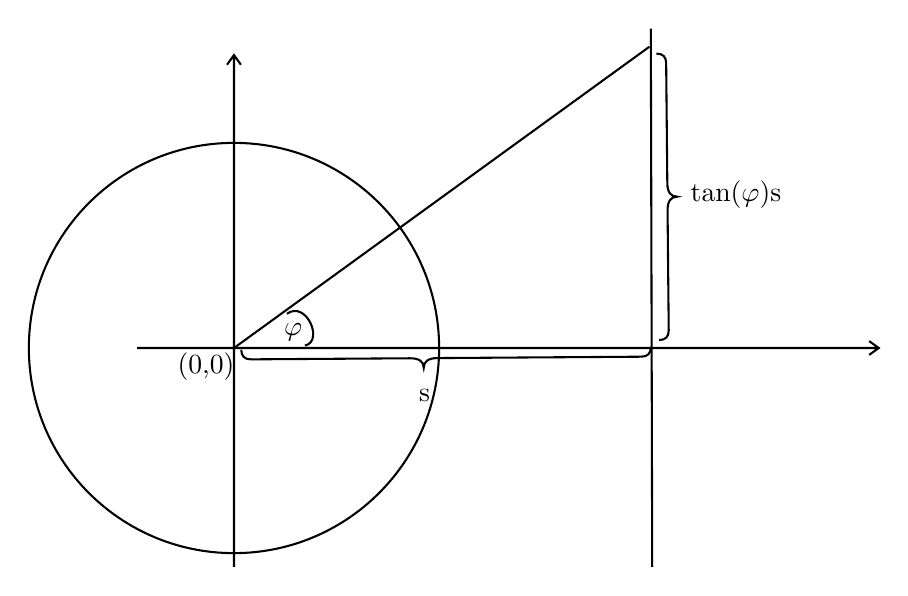
\begin{tikzpicture}[x=0.5pt,y=0.5pt,yscale=-1,xscale=1]
%uncomment if require: \path (0,444); %set diagram left start at 0, and has height of 444

%Shape: Axis 2D [id:dp6576255786763698] 
\draw  (100.32,236.75) -- (636.25,236.75)(170.25,25.01) -- (170.25,395.01) (629.25,231.75) -- (636.25,236.75) -- (629.25,241.75) (165.25,32.01) -- (170.25,25.01) -- (175.25,32.01)  ;
%Shape: Circle [id:dp3492792550747945] 
\draw   (22,236.57) .. controls (22.1,154.7) and (88.55,88.4) .. (170.43,88.5) .. controls (252.3,88.6) and (318.6,155.06) .. (318.5,236.94) .. controls (318.4,318.81) and (251.94,385.1) .. (170.06,385) .. controls (88.19,384.9) and (21.9,318.45) .. (22,236.57) -- cycle ;
%Straight Lines [id:da6321708159620955] 
\draw    (170.25,236.75) -- (470.5,19) ;


%Shape: Brace [id:dp4989740966069225] 
\draw   (175.5,238) .. controls (175.53,242.67) and (177.88,244.98) .. (182.55,244.95) -- (297.36,244.17) .. controls (304.03,244.12) and (307.37,246.43) .. (307.4,251.1) .. controls (307.37,246.43) and (310.69,244.08) .. (317.36,244.03)(314.36,244.05) -- (464.55,243.03) .. controls (469.22,243) and (471.53,240.65) .. (471.5,235.99) ;
%Curve Lines [id:da015330644298634621] 
\draw    (208.5,212) .. controls (222.5,202) and (235.5,232) .. (221.5,235) ;


%Shape: Brace [id:dp8380346617721155] 
\draw   (477.5,231) .. controls (482.17,230.95) and (484.48,228.6) .. (484.43,223.93) -- (483.6,137.43) .. controls (483.54,130.76) and (485.84,127.41) .. (490.51,127.37) .. controls (485.84,127.41) and (483.48,124.1) .. (483.41,117.43)(483.44,120.43) -- (482.58,30.93) .. controls (482.53,26.26) and (480.18,23.95) .. (475.51,24) ;
%Straight Lines [id:da8184237732199232] 
\draw    (471.5,6) -- (472.5,395) ;




\draw(150,250) node [align=left] {(0,0)};
% Text Node
\draw (308,271) node  [align=left] {s};
% Text Node
\draw (213,225) node  [align=left] {$\displaystyle \varphi $};
% Text Node
\draw (533,126) node  [align=left] {$\displaystyle \tan( \varphi )$s};
\end{tikzpicture}
\end{center}
Der Kreis ist ein zweidimensionaler Schnitt der Kugel. Es wird ein Punkt auf der rechten H\"alfte des Kreisrandes uniform gezogen (d. h. der Winkel $\varphi$ wird uniform aus $(-\frac{\pi}{2},\frac{\pi}{2})$ gezogen, $\varphi$ hat also Dichte $\frac 1 \pi \mathbf{1}_{(-\frac \pi 2, \frac \pi 2)}$). Dann wird der Laser vom Ursprung in Richtung des gezogenen Punktes auf dem Kreisrand geschossen und bis zur Mauer verl\"angert, wo dann ein bunter Punkt erscheint. Aus der Schule sollte noch bekannt sein, dass der Treffpunkt der Mauer $(s,\tan(\varphi)s)$ ist. Berechnen wir nun die Verteilung des Treffpunktes $Y$ ($y$-Achsen Abstand) auf der Mauer. Weil $\varphi\sim \mathcal U((-\frac{\pi}{2},\frac{\pi}{2}))$ ist, gilt
\begin{align*}
	\mathbb P(Y\leq t)=\mathbb P(\tan(\varphi) s\leq t)=\mathbb P(\varphi \leq \arctan(t/s))=\frac{1}{2}+\frac{1}{\pi}\arctan(t/s),
	\end{align*}
wobei in der letzten Gleichheit die Verteilungsfunktion von $\mathcal U((-\frac{\pi}{2},\frac{\pi}{2}))$ eingesetzt wurde (beachte, dass $\arctan(t/s)\in (-\frac{\pi}{2},\frac{\pi}{2})$ f\"ur alle $t,s\in\R$). Damit ist die Verteilungsfunktion von $Y$ gerade die Verteilungsfunktion von $\text{Cauchy}(s,0)$.
\end{beispiel}

Wir hatten angemerkt, dass die inverse Transformations Methode f\"ur die Normalverteilung nicht funktioniert weil $F^{-1}$ nicht explizit bekannt ist. Das n\"achste Beispiel ist daher ziemlich verbl\"uffend, die sogenante Box-Muller Methode. Man kann aus einer uniformen Zufallsvariable zwar nicht einfach eine normalverteilte Zufallsvariable bekommen, man kann aber ganz einfach aus zwei uniformen Zufallsvariablen zwei (und damit auch eine) normalverteilte bekommen! Sind $U_1, U_2$ unabh\"angige $\mathcal U([0,1])$ verteilte Zufallsvariablen, so sind 
\begin{align*}
	X_1=\cos(2\pi U_1) \sqrt{-\log(2U_2)}\quad \text{und}\quad
	X_2=\sin(2\pi U_1) \sqrt{-\log(2U_2)}
\end{align*}
zwei unabh\"angige $\mathcal N(0,1)$ Zufallsvariablen. Wer gerade noch Energie \"ubrig hat, kann mal versuchen, $\mathbb P(X_1\leq t_1,X_2\leq t_2)$ mit Polarkoordinaten auszurechnen (alle anderen k\"onnen sich das in der Monte Carlo Methoden Vorlesung anschauen). Um die Verteilung zu berechnen, solltet ihr euch an Korollar \ref{unabha} erinnern. Das Korollar besagt, dass $U_1,U_2$ und $X_1,X_2$ gemeinsame Dichten haben, n\"amlich jeweils das Produkt der einzelnen, also $\mathbf 1_{[0,1]\times [0,1]}$ bzw. $\frac{1}{2\pi} e^{-(x_1^2+x_2^2)/2}$. Damit wisst ihr, wie ihr $\mathbb P(X_1\leq t_1,X_2\leq t_2)$ durch Einsetzen der Definition ausrechnet und was rauskommen sollte.



\subsection{Summen von unabhängigen Zufallsvariablen}\label{sec:summen}
Wir berechnen nun die Verteilungen von Summen unabhängiger Zufallsvariablen. Was ist zum Beispiel die Verteilung der Summe zweier exponentialverteilter Zufallsvariablen? Oder wie ist die Summe zweier Normalverteilungen verteilt? Allgemein ist das ziemlich schwierig zu sagen, wenn die Zufallsvariablen aber unabh\"angig sind, gibt es sch\"one Rechentricks.\smallskip

Starten wir mit dem diskreten Fall, der ist einfacher. Die Idee ist einfach: Durch welche Kombination von Werten, kann die Summe $X+Y$ einen gegebenen Wert annehmen? Nat\"urlich indem $Y$ irgendeinen Wert annimmt, und $X$ gerade die Differenz zum gegebenen Wert. Wenn man alle solche M\"oglichkeiten addiert (und die Unabh\"angigkeit ausnutzt), bekommt man die diskrete Faltungsformel:
\begin{satz}\label{diskreteFaltung}
\link{https://www.youtube.com/watch?v=wJVrIDI3kTQ&list=PLy5qRKPWp6SBwfc1kn-b66cWc84cOgvqZ&index=23&t=4502s} \textbf{[Diskrete Faltungsformel]}
	Sind $X,Y$ diskrete Zufallsvariablen auf $(\Omega, \cA, \mathbb{P})$, dann ist auch $X+Y$ diskret mit m\"oglichen Werten in $X(\Omega)+Y(\Omega):=\{a+b: a\in X(\Omega), b\in Y(\Omega)\}$. Dabei bezeichnen wir mit $X(\Omega), Y(\Omega)$ die m\"oglichen Werte von $X,Y$ sind. Sind $X$ und $Y$ unabh\"angig, so k\"onnen die Wahrscheinlichkeiten mit der Faltungsformel berechnet werden:
	\[ \mathbb{P}(X+Y = k) = \sum\limits_{b \in Y(\Omega)} \mathbb{P}(X = k-b) \mathbb{P}(Y=b),\quad k\in X(\Omega)+Y(\Omega).
	\]
\end{satz}
Lasst euch nicht von der komischen Notation mit den $X(\Omega)$ und $Y(\Omega)$ irritieren, man kann die Formel einfach nicht sch\"on hinschreiben. Sobald ihr euch die folgenden Beispiele angeschaut habt, ist ganz schnell alles klar.
\begin{proof}
	Dass die Summe diskret ist und als Werte gerade Summen der Werte von $X$ und $Y$ annehmen kann, ist hoffentlich klar (denkt an zwei W\"urfel). Der Trick f\"ur die Faltungsformel ist, ein diskretes Ereigniss in eine disjunkte Vereinigung von Teilereignissen (alle M\"oglichkeiten) zu zerlegen und darauf die $\sigma$-Additivit\"at anzuwenden. Wir schreiben den Beweis einmal knapp auf, so schreibt man Argumente mit diskreten Zufallsvariablen fast immer auf, und dann noch einmal super ausf\"uhrlich, um die Ma\ss theorie dahinter zu erkennen:	
		\begin{align*}
		\mathbb{P}(X+Y = k)	
		\overset{\sigma\text{-add.}}&{=} \sum\limits_{b \in Y(\Omega)} \mathbb{P}( X + Y = k, Y = b)\\ 
		&= \sum\limits_{b \in Y(\Omega)} \mathbb{P}( X = k-b, Y = b )\\
		 \overset{\text{unab.}}&{=} \sum\limits_{b \in Y(\Omega)} \mathbb{P}(X=k-b) \mathbb{P}(Y=b).
	\end{align*}
	Die zweite Gleichheit nutzt $\sigma$-Additivit\"at weil alle M\"oglichkeiten von $Y$ ausprobiert wurden. Ganz ausf\"uhrlich sieht das gleiche Argument wie folgt aus:	
	\begin{align*}
		\mathbb{P}(X+Y =k) \overset{\text{Notation}}&{=} \mathbb{P}(\{ \omega\colon X(\omega) + Y(\omega) = k \}) \\
		\overset{\text{Trick}}&{=} \mathbb{P}\Big(\bigcupdot_{b \in Y(\Omega)} \{ \omega\colon X(\omega) + Y(\omega) = k, Y(\omega) = b \} \Big)\\
		\overset{\sigma\text{-add.}}&{=} \sum\limits_{b \in Y(\Omega)} \mathbb{P}(\{ \omega\colon X(\omega) + Y(\omega) = k, Y(\omega) = b \})\\ 
		&= \sum\limits_{b \in Y(\Omega)} \mathbb{P}(\{ \omega\colon X(\omega) = k - b, Y(\omega) = b \})\\
		\overset{\text{Notation}}&{=} \sum\limits_{b \in Y(\Omega)} \mathbb{P}(X = k - b, Y = b )\\
		 \overset{\text{unab.}}&{=} \sum\limits_{b \in Y(\Omega)} \mathbb{P}(X=k-b) \mathbb{P}(Y=b).
	\end{align*}
	Wir m\"ussen in der Mathematik immer vorsichtig sein, einfache Dinge nicht zu sehr zu verkomplizieren. Diskrete Zufallsvariablen sind ganz sicher so ein Beispiel!
\end{proof}
Als Anmerkung zum Freuen auf die strahlende Zukunft: Genau wegen dieses kleinen Tricks, kann man so sch\"on mit Markovketten rumrechnen!\smallskip

Die Formel sieht vielleicht abstrakt und unhandlich aus, wie k\"onnen aber wirklich ganz einfach in konkrete Beispielen damit rechnen:



\begin{beispiel}
\link{https://www.youtube.com/watch?v=wJVrIDI3kTQ&list=PLy5qRKPWp6SBwfc1kn-b66cWc84cOgvqZ&index=23&t=4899s}
	Sind $X_1,...,X_n$ u.i.v mit $X_1 \sim \operatorname{Ber}(p)$ f\"ur ein $p\in (0,1)$, dann gilt $X_1+...+X_n \sim \operatorname{Bin}(n,p)$. Interpretation: Wenn $\operatorname{Ber}(p)$ die erfolgreiche Ausf\"uhrung eines Versuchs ($1$=Erfolg, $0$=Misserfolg) beschreibt, so beschreibt $\operatorname{Bin}(n,p)$ die Anzahl der erfolgreichen Ausf\"uhrungen von $n$ unabhängigen Versuchen.
\end{beispiel}

\begin{proof}
	Induktion über $n$:
	\begin{itemize}
		\item[IA:] $n=1$: $\checkmark$ $\operatorname{Ber}(p) = \operatorname{Bin}(1,p)$ nach Definition beider Verteilungen.
		\item[IV:] Die Behauptung gelte für ein \textit{beliebiges}, aber festes $n \in \N$.
		\item[IS:] Indem wir $X_1+...+X_{n+1}=(X_1+...+X_n)+X_{n+1}$ klammern, wenden wir die diskrete Faltungsformel an und nutzen dann die Induktionsvoraussetzung:
		 \begin{align*}
			\mathbb{P}(X_1+...+X_{n+1} = k)
			\overset{\text{\ref{diskreteFaltung}}}&{=} \mathbb{P}(X_1+...+X_{n} = k-1) \mathbb{P}(X_{n+1} = 1)\\
			&\quad + \mathbb{P}(X_1+...+X_{n} = k) \mathbb{P}(X_{n+1} = 0)\\
			&= \left(  n\atop{k-1}\right) p^{k-1} (1-p)^{n-k+1}p + \left( n\atop k\right) p^{k} (1-p)^{n-k}(1-p) \\
			&= \left(\left( n\atop {k-1} \right) + \left( n\atop  k\right)\right) p^k (1-p)^{n-k+1}\\
			& = \left({n + 1}\atop  k \right) p^k (1-p)^{n-k+1}.
		\end{align*}
		Im letzten Schritt haben wir eine Rechnenregel f\"ur Binomialkoeffizienten benutzt, die kennt ihr vermultich aus Analysis 1. Also ist $X_1+...+X_n \sim \operatorname{Bin}(n,p)$ gezeigt. 
	\end{itemize} 
\end{proof}
\begin{beispiel}
\link{https://www.youtube.com/watch?v=wJVrIDI3kTQ&list=PLy5qRKPWp6SBwfc1kn-b66cWc84cOgvqZ&index=23&t=5571s}
	Seien $X \sim \operatorname{Poi}(\lambda), Y \sim \operatorname{Poi}(\beta)$ unabhängig. Dann ist auch $X+Y$ Poissonverteilt, und zwar mit Parameter $\lambda+\beta$. In den \"Ubungen setzt ihr einfach in die Faltungsformel ein, um $X+Y\sim \operatorname{Poi}(\lambda+\beta)$ zu zeigen. Easy.
%	\begin{align*}
%		\mathbb{P}(X+Y=n) &= \sum\limits_{k \in \N_0} \mathbb{P}(X = n-k)\mathbb{P}(Y = k)\\
%		& = \sum\limits_{k=0}^{n} e^{-\lambda} \frac{\lambda^{n-k}}{(n-k)!} e^{-\beta} \frac{\beta^{k}}{k!}\\
%		&= e^{-(\lambda + \beta)} \frac{1}{n!} \sum\limits_{k=0}^{n} \frac{n!}{(n-k)!} \lambda^{n-k} \beta^{k}\\
%		& = e^{-(\lambda + \beta)} \frac{1}{n!} \sum\limits_{k=0}^{n} \Big(\begin{array}{c} n\\ k\end{array}\Big) \lambda^{n-k} \beta^{k}\\
%		& \overset{\text{bin.}}{\underset{\text{Formel}}{=}} e^{-(\lambda + \beta)} \frac{(\lambda + \beta)^n}{n!}.
%	\end{align*}
%	Damit ist $X+Y\sim \operatorname{Poi}(\lambda+\beta)$ gezeigt.
\end{beispiel}

\begin{deff}\link{https://www.youtube.com/watch?v=wJVrIDI3kTQ&list=PLy5qRKPWp6SBwfc1kn-b66cWc84cOgvqZ&index=23&t=5954s} \abs

\begin{itemize}
\item[(i)]
	Sind $\mu_1,...,\mu_n$ Wahrscheinlichkeitsmaße auf $\cB(\R)$, so heißt das Bildmaß vom Produktmaß $\mu_1 \otimes ... \otimes \mu_n$ unter der Abbildung $h_d(x_1,...,x_d) = x_1+...+x_d$ \textbf{Faltung} der Maße. Wir schreiben $\mu_1 *...* \mu_n$ für die Faltung.
%	\begin{center}		
%		\begin{tikzcd}
%			(\cB(\R^d), \mu_1 \otimes ... \otimes \mu_n) \arrow[r, "{h_d}"] & (\cB(\R), \mu_1 \times ... \times \mu_n).
%		\end{tikzcd}
%	\end{center}
\item[(ii)]
	Sind $X_1,...,X_d$ unabhängige Zufallsvariablen auf $(\Omega, \cA, \mathbb{P})$, so heißt $\mathbb{P}_{X_1} *...*\mathbb{P}_{X_d}$ \textbf{Faltung} von $X_1, ..., X_d$.
	\end{itemize}
\end{deff}

\begin{bem1}
	Nat\"urlich ist die Definition der Faltung abstrakt, andererseits ist sie auch konkret. Die Faltung ist nichts weiter als die Verteilung der Summe unabh\"angiger Zufallsvariablen:
	\begin{align*}
		X_1+...+X_n\sim \mathbb{P}_{X_1} *...*\mathbb{P}_{X_d}.
	\end{align*}	
	Wir m\"ussen uns daf\"ur nur daran erinnern, dass die Verteilung unabh\"angiger Zufallsvariablen das Produktma\ss{} ist:
	\begin{align*}
		\mathbb{P}(X_1+...+X_d \in B) &= \mathbb{P}(X_1,...,X_d \in h_d^{-1}(B)) \\
		\overset{\text{unab.}}&{=} \mathbb{P}_{X_1} \otimes ... \otimes \mathbb{P}_{X_d}(h_d^{-1}(B))\\
		\overset{\text{Def. push-forw.}}&{=} \mathbb{P}_{X_1} *...*\mathbb{P}_{X_d}(B).
	\end{align*}
\end{bem1}
Mit der Definition der Faltung k\"onnen wir erstmal nicht viel anstellen, wir haben die Faltung schlie\ss lich einfach als das definiert, was wir berechnen wollen. Was wir gerne h\"atten, w\"are ein analog zu der diskreten Faltungsformel, weil wir damit in konkreten Beispielen rechnen k\"onnen. Hier ist die allgemeine Formel, danach konkretisieren wir diese f\"ur den Fall mit Dichten.
\begin{prop}\label{randomProp}
\link{https://www.youtube.com/watch?v=wJVrIDI3kTQ&list=PLy5qRKPWp6SBwfc1kn-b66cWc84cOgvqZ&index=23&t=6597s}
	Seien $\mu_1,\mu_2$ Wahrscheinlichkeitsmaße auf $\cB(\R)$ mit Verteilungsfunktionen $F_1,F_2$, dann gelten:
	\begin{enumerate}[label=(\roman*)]
		\item Mit $B-y: = \{ x-y\colon x \in B \}$, d. h. die Verschiebung der Menge $B$ um $y$ nach links, gilt \[ \mu_1 * \mu_2(B) = \int_{\R} \mu_1(B-y) \dint \mu_2(y)\] f\"ur alle $B\in \mathcal B(\R)$.
		\item F\"ur alle $t\in \R$ gilt \[ F_{\mu_1 * \mu_2}(t) = \int_{\R} F_1(t-y) \dint \mu_2(y).\]
	\end{enumerate}
\end{prop}
\"Uberlegt mal kurz zum Spa\ss{}, warum die verschobenen Mengen $B-y$ wieder messbar sind. \footnote{Weil $B-y$ das Urbild von B unter der messbaren (weil stetig) Abildung $z\mapsto z+y$ ist.}
\begin{proof}\abs
	\begin{enumerate}[label=(\roman*)]
		\item 
		Wegen der Manipulation
		 \[ \mathbf{1}_{B-y}(x) = \begin{cases}
		1&:x \in B-y\\
		0&:\text{sonst}
		\end{cases} = \begin{cases}
		1&: x+y \in B\\
		0&: \text{sonst}
		\end{cases} = \mathbf{1}_{h_2^{-1}(B)}(x,y) \]
		folgt
		\begin{align*}
		\mu_1 * \mu_2(B) \overset{\text{Def.}}&{=} \mu_1 \otimes \mu_2(h_2^{-1}(B)) \\
		&= \int_{\R^2} \mathbf{1}_{h_2^{-1}(B)}(x,y) \dint \mu_1\otimes \mu_2(x,y)\\
		& = \int_{\R^2} \mathbf{1}_{B-y}(x) \dint \mu_1\otimes \mu_2(x,y) \\
		\overset{\text{Fubini}}&{=} \int_{\R} \Big( \int_{\R} \mathbf{1}_{B-y}(x) \dint \mu_1(x) \Big) \mu_2(y)\\
		& = \int_{\R} \mu_1(B-y) \dint \mu_2(y).
		\end{align*}
		Das ist die erste Aussage.
		\item Wir setzten in (i) die Mengen $B = (-\infty,t]$ mit $B-y = (-\infty,t-y]$ ein, und nutzen die Definition der Verteilungsfunktion.
	\end{enumerate}
\end{proof}
Nun zur konkreten Rechenvorschrift, um die Verteilung der Summe unabh\"angiger Zufallsvariablen mit Dichten zu berechnen:
\begin{satz}
\link{https://www.youtube.com/watch?v=wJVrIDI3kTQ&list=PLy5qRKPWp6SBwfc1kn-b66cWc84cOgvqZ&index=23&t=7199s} \textbf{[Stetige Faltungsformel]}
	Sind $X,Y$ unabhängige absolutstetige Zufallsvariablen mit Dichten $f_X$, $f_Y$, dann ist auch $X+Y$ absolutstetig und hat Dichte 
	\[ f_{X+Y}(x) = \int_{\R} f_X(x-y)f_Y(y) \dint y, \quad x\in\R.\]
\end{satz}
\begin{proof}
	Mit vorheriger Proposition kennen wir die Verteilungsfunktion der Summe. Wir rechnen diese mit der Formel aus und setzen dabei die bekannten Dichten ein:
	\begin{align*}
		\mathbb{P}_{X+Y}((-\infty,t])\overset{\text{Def. Faltung}}&{=}\mathbb{P}_X * \mathbb{P}_Y((-\infty,t])\\
		 \overset{\text{\ref{randomProp}}}&{=} \int_{\R} \mathbb{P}_X ((-\infty,t-y]) \dint \mathbb{P}_Y(y) \\
		\overset{\text{\ref{IntDichten}}}&{=} \int_{\R} \int_{-\infty}^{t-y} f_X(x) \dint x f_Y(y) \dint y\\
		 \overset{\text{Subst.}}&{=} \int_{\R} \int_{-\infty}^{t} f_X(x-y) \dint x f_Y(y) \dint y\\
		&= \int_{\R} \int_{\R} \mathbf{1}_{(-\infty,t]}(x) f_X(x-y) f_Y(y) \dint x \dint y\\
		 \overset{\text{Fubini}}&{=} \int_{-\infty}^{t} \int_{\R} f_X(x-y) f_Y(y) \dint y \dint x\\
		&= \int_{-\infty}^t f_{X+Y}(x)\dint x.	
	\end{align*}
	Also ist $X+Y$ absolutstetig mit behaupteter Dichte $f_{X+Y}$.
\end{proof}

	Das Konzept der Faltung kommt nicht aus der Stochastik, daher k\"onnen wir mit dem Begriff \enquote{Faltung} auch nichts anfangen. Die Faltung zweier integrierbarer Funktionen wird in der Fourieranalysis als 
	\begin{align*}
		f\ast g (x)=\int_\R f(x-y) g(y)\dint y,\quad x\in\mathbb R,
	\end{align*}
	definiert und zum Beispiel in der Signalverarbeitung studiert. Dass die Faltung bei uns f\"ur Summen unabh\"angiger Zufallsvariablen auftaucht, ist ein Zufall der Mathematik. Es gibt also keinen Grund sich Gedanken \"uber die Begrifflichkeit Faltung zu machen, f\"ur uns ist es einfach nur eine Berechnungsformel.
\marginpar{\textcolor{red}{Vorlesung 23}}



\begin{beispiel}\label{B5} \link{https://www.youtube.com/watch?v=lxTw3_a68yw&list=PLy5qRKPWp6SBwfc1kn-b66cWc84cOgvqZ&index=24&t=0s} \abs

	\begin{enumerate}[label=(\roman*)]\label{bspFaltung}
		\item Sind $X_1 \sim \cN(\mu_1,\sigma_1^2)$ und $X_2 \sim \cN(\mu_2,\sigma_2^2)$ unabhängig, dann ist auch die Summe wieder normalverteilt, genauer, es gilt $X_1 + X_2 \sim \cN(\mu_1 + \mu_2, \sigma_1^2 + \sigma_2^2)$. Das kann man mit der stetigen Faltungsformel ausrechnen:
		\begin{align*}
			f_{X_1 + X_2}(x) &= \int_{\R} \frac{1}{\sqrt{2 \pi \sigma_1^2}} e^{-\frac{(x-y-\mu_1)^2}{2\sigma_1^2}} \frac{1}{\sqrt{2 \pi \sigma_2^2}} e^{-\frac{(y-\mu_2)^2}{2\sigma_2^2}} \dint y\\
			&=\frac{1}{\sqrt{2\pi(\sigma_1^2+\sigma_2^2)}} e^{-\frac{(x-(\mu_1+\mu_2))^2}{2(\sigma_1^2+\sigma_2^2)}},\quad x\in\R.
		\end{align*}
		Auf den ersten Blick ist nicht so klar, ob die Berechnung einfach oder nicht so einfach ist. Im Prinzip muss man nur richtig quadratisch erg\"anzen und Substituieren. In der Tat ist die Rechnung ziemlich b\"ose, klappt aber. Weil wir gleich eine viel einfachere Methode kennenlernen, lassen wir die Rechnung weg.
		\item Sind $X_1 \sim \operatorname{Exp}(\lambda), X_2 \sim \operatorname{Exp}(\lambda)$ unabhängig, so ist $X_1+ X_2 \sim \Gamma(2,\lambda)$. Das kann man direkt mit der stetigen Faltungsformel ausrechnen:
		\begin{align*}
			f_{X_1+X_2}(x)&=\int_\R  f_{X_1}(x-y) f_{X_2}(y)\dint y\\
			 &=\int_\R \mathbf 1_{[0,\infty)}(x-y) \lambda e^{-\lambda (x-y)} \mathbf 1_{[0,\infty)}(y) \lambda e^{-\lambda y}\dint y\\
			&=\lambda^2 \int_0^x e^{-\lambda x} \dint y=\lambda^2 x e^{-\lambda x}.
		\end{align*}
\end{enumerate}
\end{beispiel}

Jetzt noch eine ganz andere Methode zur Berechnung der Verteilung der Summe von unabh\"angigen Zufallsvariablen. Daf\"ur nutzen wir einen Satz der Wahrscheinlichkeitstheorie, den Eindeutigkeitssatz f\"ur momenterzeugende Funktionen. Der Satz besagt, dass Verteilungen eindeutig durch ihre momenterzeugenden Funktionen festgelegt sind, falls diese um $0$ existieren.
\begin{satz}\label{WT}
\link{https://www.youtube.com/watch?v=lxTw3_a68yw&list=PLy5qRKPWp6SBwfc1kn-b66cWc84cOgvqZ&index=24&t=805s}
	Seien $X$ und $Y$ Zufallsvariablen f\"ur die die momenterzeugenden Funktionen $\cM_X,\cM_Y$ in $(-\varepsilon,\varepsilon)$ existieren für ein $\varepsilon > 0$. Falls $\cM_X(t) = \cM_Y(t)$ für alle $t \in (-\varepsilon,\varepsilon)$ gilt, so gilt $X\sim Y$.
	\end{satz}
\begin{proof}
	Siehe fortgeschrittene Stochastikvorlesung - hart!
\end{proof}
F\"ur Verteilungen mit expliziten momenterzeugenden Funktionen ist diese ein extrem n\"utzliches Hilfsmittel. 
\begin{beispiel}\label{B55}
\link{https://www.youtube.com/watch?v=lxTw3_a68yw&list=PLy5qRKPWp6SBwfc1kn-b66cWc84cOgvqZ&index=24&t=936s}
	Mit der momenterzeugenden Funktion k\"onnen wir ganz einfach die Skalierungseigenschaft der Normalverteilung zeigen: Ist $X\sim \mathcal N(0,1)$, $\mu\in \R$ und $\sigma^2>0$, so gilt $Y:=\sigma X+\mu \sim \mathcal N(\mu,\sigma^2)$. Rechnen wir dazu die momenterzeugende Funktion von $Y$ aus:
	\begin{align*}
		M_Y(t)=\E[e^{(\sigma X  + \mu)t}]=\E[e^{\sigma t X}]e^{\mu t}=M_{X}(\sigma t)\cdot e^{\mu t}= e^{\frac{\sigma^2 t^2}{2}+\mu t},\quad t\in \R,
	\end{align*}
	und die rechte Seite ist gerade die momenterzeugende Funktion einer $\mathcal N(\mu, \sigma^2)$-verteilten Zufallsvariable. Also folgt die Behauptung aus Satz \ref{WT}.
\end{beispiel}


Gemeinsam mit folgender Proposition ist Satz \ref{WT} ein m\"achtiges Hilfsmittel um die Verteilung Summen unabh\"angiger Zufallsvariablen zu berechnen:
\begin{prop}\label{P7}
\link{https://www.youtube.com/watch?v=lxTw3_a68yw&list=PLy5qRKPWp6SBwfc1kn-b66cWc84cOgvqZ&index=24&t=1375s}
	Sind $X$ und $Y$ unabhängige Zufallsvariablen mit $\cM_X(t),\cM_Y(t) < \infty$ f\"ur ein $t\in\R$, so gilt auch $\cM_{X+Y}(t) = \cM_X(t)\cM_Y(t)$.
\end{prop}

\begin{proof} 
Das folgt direkt daraus, dass Erwartungswerte von Produkten unabh\"angiger Zufallsvariablen faktorisieren, siehe Satz \ref{un}:
	$$\cM_{X+Y}(t) = \E[e^{t(X+Y)}] = \E[e^{tX}\cdot e^{tY}] = \E[e^{tX}] \cdot \E[e^{tY}] = \cM_X(t)\cM_Y(t).$$
\end{proof}

Die Anwendung der momenterzeugenden Funktion zur Bestimmung der Verteilung von Summen unabh\"angiger Zufallsvariablen versteht man am besten mit folgendem einfachen Beispiel. Beachte: Das Beispiel ist einfach, die Aussage aber nicht. H\"atten wir nicht die Kanone aus der Wahrscheinlichkeitstheorie ausgepackt, h\"atten wir das mit der stetigen Faltungsformel nachrechnen m\"ussen. 

\begin{beispiel}\label{momg}
\link{https://www.youtube.com/watch?v=lxTw3_a68yw&list=PLy5qRKPWp6SBwfc1kn-b66cWc84cOgvqZ&index=24&t=1661s}
	Kommen wir zur\"uck zu Beispiel \ref{B5} (i) und berechnen mit der Proposition die momenterzeugende Funktion der Summe der zwei unabh\"angigen Normalverteilungen. Wegen Proposition \ref{P7} und der in den \"Ubungen berechneten Formel f\"ur die momenterzeugende Funktion einer Normalverteilung gilt
	\begin{gather*}
		\cM_{X_1+X_2}(t) = \cM_{X_1}(t)\cM_{X_2}(t) = e^{\mu_1 t + \frac{\sigma_1^2}{2}t^2} e^{\mu_2 t + \frac{\sigma_2^2}{2}t^2}=e^{(\mu_1+\mu_2)t + \frac{\sigma_1^2 + \sigma_2^2}{2}t^2},\quad t\in\R.
	\end{gather*}
	Nun wissen wir aber auch, dass
	\begin{align*}
		\cM_Y(t)=e^{(\mu_1+\mu_2)t + \frac{\sigma_1^2 + \sigma_2^2}{2}t^2}, \quad t\in\R,
	\end{align*} 
	 f\"ur $Y \sim \cN(\mu_1 + \mu_2, \sigma_1^2 + \sigma_2^2)$. Also gilt $X_1+X_2\sim Y$ nach Satz \ref{WT} und damit gilt f\"ur die Summe $X_1+X_2\sim \mathcal N(\mu_1+\mu_2,\sigma_1^2 + \sigma_2^2)$.
\end{beispiel}
Mit \"ahnlichen Rechnungen kann man (siehe \"Ubungen) mit momenterzeugenden Funktionen auch zeigen, dass
\begin{itemize}
	\item die Summe unabh\"angiger Exponentialverteilungen gammaverteilt ist,
	\item die Summe unabh\"angiger Gammaverteilungen wieder gammaverteilt ist,
	\item die Summe unabh\"angiger Bernoulliverteilungen binomialverteilt ist (haben wir oben schon mit der Faltungsformel berechnet),
\end{itemize}
Das Argument ist immer identisch: Berechne die momenterzeugende Funktion der Summe als Produkt der momenterzeugenden Funktionen der einzelnen (Unabh\"angigkeit) und hoffe, dass das Produkt eine bereits bekannt momenterzeugende Funktion ist. Dann kann die Verteilung der Summe mittels Satz \ref{WT} identifiziert werden. 
\begin{bem}
\link{https://www.youtube.com/watch?v=lxTw3_a68yw&list=PLy5qRKPWp6SBwfc1kn-b66cWc84cOgvqZ&index=24&t=2038s}
\abs
\begin{itemize}
\item Der Trick mit der Normalverteilung funktioniert aufgrund der Faktorisierungseigenschaft der Exponentialfunktion. Wir sehen also, dass der Trick auf Situationen beschr\"ankt ist, wenn in einer n\"utzlichen Form Potenzen auftauchen. 
\item Die Vorlesung ist hier etwas irref\"uhrend. Satz \ref{WT} ist kein Allheilmittel. In der (mathematischen) Realit\"at sind exponentielle Momente sehr oft unendlich und wir k\"onnen nicht mit der momenterzeugenden Funktion arbeiten. In dieser Vorlesung sind alle Verteilungen au\ss er Cauchy und Exponentiell unproblematisch, weil alle exponentiellen Momente existieren. In der Wahrscheinlichkeitstheorie werden wir das Problem l\"osen, indem wir die Momenterzeugende Funktionen durch sogenannte charakteristische Funktionen $\varphi(t)=\E[e^{itX}]$ ersetzen. 
\end{itemize}
\end{bem}


\section{Bedingte Wahrscheinlichkeiten und Unabhängigkeit}\label{Sunab}
Wir kommen nun zu bedingten Wahrscheinlichkeiten, die aus der Schule vielleicht bekannt sind. In dieser Vorlesung spielen bedingte Wahrscheinlichkeiten noch keine zentrale Rolle, das \"andert sich in sp\"ateren Vorlesungen sehr, wenn zum Beispiel Markovketten angeschaut werden.
\begin{deff}
\link{https://www.youtube.com/watch?v=lxTw3_a68yw&list=PLy5qRKPWp6SBwfc1kn-b66cWc84cOgvqZ&index=24&t=2237s}
	Sei $(\Omega, \cA, \mathbb P)$ ein Wahrscheinlichkeitsraum und $A, B \in \cA$ mit $ \mathbb P(B)> 0$. Dann heißt \[ \mathbb{P}(A|B) := \frac{\mathbb{P}(A \cap B)}{\mathbb{P}(B)}\]
	\textbf{bedingte Wahrscheinlichkeit von $A$ gegeben $B$}.	
\end{deff}

\begin{lemma}
\link{https://www.youtube.com/watch?v=lxTw3_a68yw&list=PLy5qRKPWp6SBwfc1kn-b66cWc84cOgvqZ&index=24&t=2334s}
	Für $ B \in \cA$ mit $ \mathbb{P}(B)> 0$ ist $ A \mapsto \mathbb{P}(A|B) =: \mathbb{P}_B(A)$ ein Maß auf $(\Omega, \cA)$.
\end{lemma}

\begin{proof}
	Wir rechnen die definierenden Eigenschaften eines Ma\ss es nach:
	\begin{itemize}
		\item $\mathbb P_B(A) \geq 0$ f\"ur alle $A\in \mathcal A$ ist klar, weil $\mathbb P$ ein Ma\ss{} ist.
		\item Weil $\mathbb P$ ein Ma\ss{} ist, gilt auch 
		\[ \mathbb{P}_B(\emptyset) = \mathbb{P}(\emptyset|B) = \frac{\mathbb{P}(\emptyset \cap B)}{\mathbb{P}(B)} = 0. \]
		\item $\sigma$-Additivität: Seien $A_1,A_2,... \in \cA$ disjunkt, so gilt wegen der $\sigma$-Additivit\"at von $\mathbb P$
		\begin{align*}
			\mathbb{P}_B\big(\bigcupdot_{k=1}^{\infty} A_k \big) \overset{\text{Def.}}&{=} \frac{\mathbb{P}\big(\bigcupdot_{k=1}^{\infty} A_k \cap B\big)}{\mathbb{P}(B)}\\
			&= \frac{\mathbb{P}\big(\bigcupdot_{k=1}^{\infty} (A_k \cap B) \big)}{\mathbb{P}(B)} \\
			\overset{\sigma\text{-Add. }}&{=} \frac{\sum\limits_{k=1}^{\infty} \mathbb{P}(A_k \cap B)}{\mathbb{P}(B)}
			= \sum\limits_{k=1}^{\infty} \mathbb{P}_B(A_k).
		\end{align*}
	\end{itemize}
\end{proof}
Wir kommen nun zu extrem wichtigen Rechenregeln, obwohl diese ganz einfach aus der Definition folgen:
\begin{satz}\label{formelnp} \link{https://www.youtube.com/watch?v=lxTw3_a68yw&list=PLy5qRKPWp6SBwfc1kn-b66cWc84cOgvqZ&index=24&t=2512s} \abs

	\begin{enumerate}[label=(\roman*)]
		\item \label{multipl} \textbf{Multiplikationsregel}: Für $A_1,...,A_n\in \mathcal A$ mit $\mathbb{P}(\bigcap_{k=1}^{n} A_k) > 0$ gilt
		\[ \mathbb{P}\Big(\bigcap_{k=1}^{n} A_k\Big) = \mathbb{P}(A_1)\cdot \mathbb{P}(A_2|A_1)\cdot ... \cdot \mathbb{P}\Big(A_n\Big|\bigcap_{k=1}^{n-1} A_k\Big). \]
		\item \label{totWk} \textbf{Formel der totalen Wahrscheinlichkeit}: Ist $B_1,...,B_n\in \mathcal A$ eine disjunkte Zerlegung von $\Omega$, \mbox{d. h.}  $\bigcupdot_{k=1}^{n} B_k = \Omega$, mit $\mathbb P(B_k)>0$ f\"ur alle $k=1,...,n$, so gilt 
		\[ \mathbb{P}(A) = \sum\limits_{k=1}^{n} \mathbb{P}(B_k)\mathbb{P}(A|B_k), \quad \forall A \in \cA. \]
		\item \label{bayes} \textbf{Bayes-Formel}: Mit $B_1,...,B_n$ aus \ref{totWk} gilt für $A \in \cA$ mit $\mathbb{P}(A) > 0$ \[ \mathbb{P}(B|A) = \frac{\mathbb{P}(A|B) \cdot \mathbb{P}(B)}{\mathbb{P}(A)},\quad \forall B\in \mathcal A, \] oder \[ \mathbb{P}(B|A) = \frac{\mathbb{P}(A|B) \cdot \mathbb{P}(B)}{\sum\limits_{k=1}^{n} \mathbb{P}(B_k) \mathbb{P}(A | B_k)},\quad \forall B\in \mathcal A. \]
	\end{enumerate}
\end{satz}

\begin{proof}
	\begin{enumerate}[label=(\roman*)]
		\item Induktion über $n$:
		\begin{itemize}
			\item[IA:] $n=2$ folgt direkt aus der Definition der bedingten Wahrscheinlichkeit.
			\item[IV:] \label{IVmult} Die Behauptung gelte für ein \textit{beliebiges}, aber festes $n \in \N$.
			\item[IS:] Wenn wir nun die Induktionsvoraussetzung und den Fall $n=2$ nutzen, so bekommen wir 
			\begin{align*}
				\mathbb{P}\Big(\bigcap_{k=1}^{n+1} A_k\Big) &= \mathbb{P}\Big(\bigcap_{k=1}^{n} A_k\cap A_{n+1}\Big)\\
				& = \mathbb{P}\Big(\bigcap_{k=1}^{n} A_k\Big) \mathbb{P}\Big(A_{n+1}\Big |\bigcap_{k=1}^{n} A_k\Big)\\
				& \overset{\text{IV}}{=} \mathbb{P}(A_1)\cdot \mathbb{P}(A_2|A_1)\cdot ... \cdot \mathbb{P}\Big(A_{n+1}\Big|\bigcap_{k=1}^{n} A_k\Big)
			\end{align*}
			und das ist gerade die Aussage.
		\end{itemize}
		\item 
		Zun\"achst folgt direkt aus der Definition
		\begin{align*}
			\mathbb{P}(B_k)\mathbb{P}(A|B_k) = \mathbb{P}(B_k) \frac{\mathbb{P}(A \cap B_k)}{\mathbb{P}(B_k)} = \mathbb{P}(A \cap B_k).
		\end{align*}
		Setzen wir dies in folgende Rechnung ein, so bekommen wir die Aussage:
		\begin{align*}
			\mathbb{P}(A) = \mathbb{P}(A \cap \Omega) = \mathbb{P}\Big(A \cap \bigcupdot_{k=1}^{n} B_k\Big) = \mathbb{P}\Big(\bigcupdot_{k=1}^{n} (A \cap B_k)\Big)
			\overset{\sigma\text{-Add.}}{=} \sum\limits_{k=1}^{n} \mathbb{P}(A \cap B_k).
		\end{align*}
		\item Die einfache Bayes-Formel folgt direkt durch Einsetzen der Definition und Erweitern:
		\[ \mathbb{P}(B|A) = \frac{\mathbb{P}(A \cap B)}{\mathbb{P}(A)} = \frac{\mathbb{P}(A \cap B) \mathbb{P}(B)}{\mathbb{P}(B) \cdot \mathbb{P}(A)} =\frac{\mathbb{P}(A|B) \cdot \mathbb{P}(B)}{\mathbb{P}(A)} \]
		Ganz Aufmerksame werden merken, dass wir bei $\mathbb P(B)=0$ durch null geteilt haben. Das geht nat\"urlich nicht! Ist aber kein Problem, weil die Bayes-Formel in dem Fall als $0=0$ ohnehin gilt. Wir k\"onnen also ohne Einschr\"ankung $\mathbb P(B)>0$ annehmen und dann taucht das Problem nicht auf.\smallskip

		Die zweite Formel folgt aus der ersten Formel durch Ersetzen des Nenners durch die Formel der totalen Wahrscheinlichkeit. 
	\end{enumerate}
\end{proof}
Kommen wir nun zu zwei klassischen Anwendungen. Hier ist allerdings etwas Vorsicht angesagt, das ist alles etwas wild (funktioniert aber). Gem\"a\ss{} Definition brauchen wir f\"ur bedingte Wahrscheinlichkeiten einen Wahrscheinlichkeitsraum $(\Omega, \mathcal A, \mathbb P)$. In vielen Anwendungen au\ss erhalb der Mathematik werden die Formeln allerdings auch genutzt, ohne einen Wahrscheinlichkeitsraum hinzuschreiben. Nennen wir das vielleicht \enquote{heuristischen Gebrauch von Wahrscheinlichkeiten}. Das ist nat\"urlich nicht sehr sch\"on, allerdings sind solche Aussagen extrem wichtig. 

\begin{beispiel}\link{https://www.youtube.com/watch?v=lxTw3_a68yw&list=PLy5qRKPWp6SBwfc1kn-b66cWc84cOgvqZ&index=24&t=3627s} \abs

	\begin{enumerate}[label=(\roman*)]
		\item Wir ziehen aus vier blauen und drei weißen Kugeln zweimal ohne Zurücklegen. Was ist die Wahrscheinlichkeit, zwei blaue zu ziehen? Machen wir das ganze zun\"achst \enquote{heuristisch}. Das ist ein zweistufiges Experiment. Im ersten Versuch ziehen wir blau mit Wahrscheinlichkeit $\frac{4}{7}$. Mit dem Wissen im ersten Zug blau gezogen zu haben, ist das \enquote{bedingte Ziehen} im zweiten Schritt ein Ziehen aus drei blauen und drei wei\ss en Kugeln. Die bedingte Wahrscheinlichkeit im zweiten Schritt blau zu ziehen, gegeben das erste Ziehen gab eine blaue Kugel, ist also $\frac{3}{6}$. Mit der Multiplikationsregel folgt
		\begin{align*} 
		&\quad \mathbb{P}(\text{beide Kugeln blau}) \\
		&= \mathbb{P}(\text{erste Kugel blau}) \cdot \mathbb{P}(\text{zweite Kugel blau} \: | \: \text{erste Kugel blau})\\
		& = \frac{4}{7}\cdot \frac{3}{6} = \frac{2}{7}.
		\end{align*}
		Das funktioniert ganz entspannt, ist aber schon etwas kritisch. Wir nutzen hier ganz intuitiv den Begriff der bedingten Wahrscheinlichkeit in einem interpretierten Sinn (\"Anderung des Modells, eine Kugel weniger). Dann haben wir die Multiplikationsregel genutzt, die aufgrund unseres Beweises und damit aufgrund der mathematischen Definition der bedingten Wahrscheinlichkeit stimmt. Nun ist allerdings nicht so ganz klar, warum der intuitive Begriff der bedingten Wahrscheinlichkeit (ge\"andertes Experiment) mit der mathematischen Definition $\mathbb P(A\,|\,B):=\frac{\mathbb P(A\cap B)}{\mathbb P(B)}$ \"uberhaupt etwas zu tun hat. Machen wir das ganze zur Beruhigung also nochmal mathematisch penibel genau. Schreiben wir zun\"achst ein Modell hin, das wir als Modell f\"ur das zweifache W\"urfeln plausibel finden. Dazu sei
		$$\Omega = \{ (\omega_1,\omega_2)\colon \omega_1, \omega_2 \in \{ \text{blau, weiß} \} \}$$
		und $\cA = \cP(\Omega)$. Als Wahrscheinlichkeiten definieren wir
		\[ \mathbb{P}(\{ \omega_1, \omega_2 \}) = \begin{cases}
		\frac{4}{7} \cdot \frac{3}{6}&: \omega_1 = \omega_2 = \text{blau}\\
		\frac{3}{7} \cdot \frac{2}{6}&: \omega_1 = \omega_2 = \text{weiß}\\
		\frac{4}{7} \cdot \frac{3}{6}&: \omega_1 = \text{blau}, \: \omega_2 = \text{weiß}\\		
		\frac{3}{7} \cdot \frac{4}{6}&: \omega_1 = \text{weiß}, \: \omega_2 = \text{blau}\\
		\end{cases}. \]
		Mit den Ereignissen 		
		$A = \{ (\omega_1, \omega_2)\colon \omega_1 = \text{blau} \}$, $B = \{ (\omega_1, \omega_2)\colon \omega_2 = \text{blau} \}$
		wollen wir die Wahrscheinlichkeit von $A\cap B$ bestimmen. Mit der Multiplikationsregel folgt
		\begin{align*}
			\mathbb{P}(\text{ziehe zweimal blau}) = \mathbb{P}(A \cap B) = \mathbb{P}(A) \cdot \mathbb{P}(B|A) =  \frac{4}{7} \cdot \frac{\mathbb{P}(A \cap B)}{\mathbb{P}(A)} = \frac{2}{7}.
		\end{align*}
		Das macht nat\"urlich auch wieder nicht so richtig viel Sinn, wir h\"atten die Wahrscheinlichkeit von $A\cap B$ auch ohne die Multiplikationsregel \enquote{ablesen} k\"onnen. Dennoch ist das vielleicht eine gute Beruhigung: Wenn wir wollen, k\"onnen wir ein rigoroses Modell hinschreiben, in dem die Multiplikationsformel rigoros gemacht werden kann. F\"ur die Schulanwendungen ist das nat\"urlich viel zu kompliziert.		
		\item Nun ein Beispiel f\"ur die Bayes-Formel, ein medizinischer Test, \mbox{z. B.} ein Aidstest. Wir machen das jetzt wieder in der \enquote{heuristischen} Art, wer will, kann sich wieder ein sauberes Modell definieren. Wir nehmen an, dass die Wahrscheinlichkeiten folgender Ereignisse bekannt sind:
		\begin{itemize}
			\item $1\%$ der Bevölkerung ist tats\"achlich krank.
			\item Test ist mit $98\%$ positiv, wenn eine Person krank ist.
			\item Test ist mit $5\%$ positiv, wenn eine Person nicht krank ist, das nennt mann false-positive (Fehlalarm).
		\end{itemize}
		Gesucht ist die Wahrscheinlichkeit gesund zu sein, obwohl der Test positiv ist. Mit der Bayes-Formel gilt
		\begin{align*}
			&\quad \mathbb{P}(\text{krank} \: | \: \text{Test positiv})\\
			 &= \mathbb{P}(\text{Test positiv} \: | \: \text{krank}) \cdot \frac{\mathbb{P}(\text{krank})}{\mathbb{P}(\text{Test positiv})}\\
			&=	\frac{\mathbb{P}(\text{Test positiv} \: | \: \text{krank}) \mathbb{P}(\text{krank})}{\mathbb{P}(\text{Test positiv} \: | \: \text{krank})\mathbb{P}(\text{krank}) + \mathbb{P}(\text{Test positiv} \: | \: \text{gesund})\mathbb{P}(\text{gesund})}\\
			&= \frac{0,98 \cdot 0,01}{0,98 \cdot 0,01 + 0,05 \cdot 0,99} \\
			&= 0,165.
		\end{align*}
		Das ergibt dann
		\begin{align*}
			\mathbb{P}(\text{gesund} \: | \: \text{Test positiv}) = 1 - 0,165 = 0,835,
		\end{align*}
		was erschreckend hoch ist! Die wichtige take-home message ist also: Wird etwas sehr unwahrscheinliches getestet, dominieren falsche Tests und man muss bei positiven Tests unbedingt weitere Tests machen. Ein weiteres sehr wichtiges Beispiel sind pr\"anatale Tests bei ungeborenen Kindern, z. B. Tests auf Trisomie 21 (auf die moralische Frage wollen wir hier nat\"urlich nicht eingehen!).
	\end{enumerate}
\end{beispiel}
Weiter geht es jetzt mit einer mathematischen Definition von Unabh\"angigkeit von Ereignissen. Ihr habt sicherlich eine naive Vorstellung \glqq Hat nichts mit einander zu tun\grqq. Beispielsweise w\"aren die Ereignisse \enquote{Meine Kaffeemaschiene geht morgen kaputt} und \enquote{Es regnet morgen in Thailand} vermutlich unabh\"angig. Hier ist eine Definition:
\begin{deff}\label{def:unab}
\link{https://www.youtube.com/watch?v=lxTw3_a68yw&list=PLy5qRKPWp6SBwfc1kn-b66cWc84cOgvqZ&index=24&t=4799s}
	Sei $(\Omega, \cA, \mathbb{P})$ ein Wahrscheinlichkeitsraum und seien $A,B \in \cA$. Die Ereignisse $A$ und $B$ heißen \textbf{unabhängig}, falls $\mathbb{P}(A \cap B) = \mathbb{P}(A) \cdot \mathbb{P}(B)$.
\end{deff}
Aufgrund der Definition der bedingten Wahrscheinlichkeit sind, sofern $\mathbb P(B)>0$ gilt, $A$ und $B$ unabh\"angig genau dann, wenn $\mathbb P(A|B)=P(A)$. Das passt also zur Begriffsbildung: Zwei Ereignisse sind genau dann unabh\"angig, falls die Wahrscheinlichkeit des einen sich nicht \"andert, wenn das Eintreten des anderen gegeben ist.\smallskip

Oft braucht man auch die Unabh\"angigkeit mehrerer Ereignisse. F\"ur endlich viele ist klar was man macht, die Wahrscheinlichkeit des endlichen Schnittes soll nat\"urlich das endlich Produkt sein. F\"ur unendlich viele ist das problematisch, darum f\"uhrt man alles auf endlich viele zur\"uck:
\begin{deff}
\link{https://www.youtube.com/watch?v=lxTw3_a68yw&list=PLy5qRKPWp6SBwfc1kn-b66cWc84cOgvqZ&index=24&t=5109s}
	Sei $(\Omega, \cA, \mathbb{P})$ ein Wahrscheinlichkeitsraum, $A_i \in \cA$, $i \in I$, und $I$ eine beliebige Indexmenge.
	\begin{enumerate}[label=(\roman*)]
		\item Die Ereignisse ${(A_i)}_{i\in I}$ heißen \textbf{unabhängig}, falls 
		\[ \mathbb{P}\big(\bigcap_{i \in J} A_i \big) = \prod\limits_{i \in J} \mathbb{P}(A_i),\quad \forall J \subseteq I \text{ mit }  \# J<\infty. \]
		\item Die Ereignisse ${(A_i)}_{i\in I}$ heißen \textbf{paarweise unabhängig}, falls 
		$$\mathbb{P}(A_i \cap A_j) = \mathbb{P}(A_i) \cdot \mathbb{P}(A_j), \quad \forall i\neq j.$$
	\end{enumerate}
\end{deff}
Selbstverst\"andlich impliziert Unabh\"angikgkeit die paarweise Unabh\"angigkeit, statt aller endlicher Teilmengen $J$ von $I$ werden schlie\ss lich nur alle Teilmengen mit $\# J=2$ gew\"ahlt. Die Umkehrung gilt nicht:
\begin{warnung}
\link{https://www.youtube.com/watch?v=lxTw3_a68yw&list=PLy5qRKPWp6SBwfc1kn-b66cWc84cOgvqZ&index=24&t=5304s}
	Paarweise Unabhängigkeit impliziert im Allgemeinen nicht Unabhängigkeit. Kleine Mengen reichen schon aus, um Gegenbeispiel anzugeben, siehe \"Ubungsblatt.
\end{warnung}
In Worten ausgedr\"uckt hei\ss t die Unabh\"angigkeit auch \glqq Die Ereignisse ${(A_i)}_{i\in I}$ sind unabh\"angig, falls jede Wahl von endlich vielen Ereignissen $A_{i_1},...,A_{i_n}$ unabh\"angig ist\grqq.\smallskip

Als n\"achstes wollen wir die Unabh\"angigkeit von $\sigma$-Algebren und Zufallsvariablen thematisieren. Dazu zun\"achst eine allgemeinere Definition:
\begin{deff}\label{Ka}
\link{https://www.youtube.com/watch?v=lxTw3_a68yw&list=PLy5qRKPWp6SBwfc1kn-b66cWc84cOgvqZ&index=24&t=5374s}
	Sei $(\Omega, \cA, \mathbb{P})$ ein Wahrscheinlichkeitsraum und ${(\cE_i)}_{i \in I}$ eine Familie von Teilmengen $\cE_i \subseteq \cA$ der $\sigma$-Algebra f\"ur eine beliebige Indexmenge $I$. Dann heißen die $(\cE_i)_{i\in I}$ unabhängig, falls die Ereignisse ${(A_i)}_{i \in I}$ unabhängig sind, und zwar f\"ur alle $A_i \in \cE_i$.
\end{deff}


Die Definition wird insbesondere f\"ur $\sigma$-Algebren verwendet. Wie bei der Messbarkeit fragen wir uns hier, ob wir die Unabh\"angigkeit auf Erzeuger reduzieren k\"onnen. Wie immer funktioniert das, zumindest wenn der Erzeuger $\cap$-stabil ist:
\begin{prop}\label{unabh}
\link{https://www.youtube.com/watch?v=lxTw3_a68yw&list=PLy5qRKPWp6SBwfc1kn-b66cWc84cOgvqZ&index=24&t=5613s}
	Ist $(\Omega, \cA, \mathbb{P})$ ein Wahrscheinlichkeitsraum und $\cE_i \subseteq \cA$ für f\"ur alle $i \in I$. Sind alle $\cE_i$ $\cap$-stabil, so gilt:
	\begin{align*}
		(\cE_i)_{i\in I}\text{ unabhängig }\quad \Leftrightarrow\quad  (\sigma(\cE_i))_{i \in I}\text{ unabhängig.}
	\end{align*}
\end{prop}

\begin{proof}\abs
	\begin{itemize}
		\item[\enquote{$\Leftarrow$}:] Klar nach Definition, weil $\cE_i \subseteq \sigma(\cE_i)$ gilt. Die Unabh\"angigkeit von Mengensystemen bedeutet schlie\ss lich, dass die Unabh\"angigkeit f\"ur alle Auswahlen von Teilmengen gilt. Gilt dies f\"ur mehr M\"oglichkeiten, so nat\"urlich auch f\"ur weniger M\"oglichkeiten.
		\item[\enquote{$\Rightarrow$}:] Ohne Einschr\"ankung sei $I$ endlich weil die Definition der Unabh\"angkigkeit nur auf endlichen Teilmengen $J \subseteq I$ beruht. Nennen wir die Mengen $\cE_1,...,\cE_n$. Wir zeigen, dass dann auch $\sigma(\cE_1),...,\sigma(\cE_n)$ unabhängig sind. Dazu zeigen wir zun\"achst:
		$$\cD:= \big\{ E \in \cA \colon \{ E \}, \cE_2, ..., \cE_n \text{ sind unabhängig} \big\}\text{ ist ein Dynkin-System.}$$
		Um das zu zeigen, checken wir die definierenden Eigenschaften eines Dynkin-Systems:
		\begin{enumerate}[label=(\roman*)]
			\item Aufgrund der Definition \ref{Ka} m\"ussen wir zeigen, dass f\"ur alle $ A_2 \in \cE_2,...,A_n \in \cE_n$ die Mengen $\Omega, A_2,...,A_n$ unabhängig sind, die Wahrscheinlichkeit vom Schnitt also zur Wahrscheinlichkeiten der einzelnen Ereignisse faktorisiert. Das folgt aber direkt aus der angenommenen Unabh\"angigkeit von $\mathcal E_1, ..., \mathcal E_n$:			
			\begin{align*}
				\mathbb{P}(\Omega \cap A_2 \cap ... \cap A_n) &= \mathbb{P}(A_2 \cap ... \cap A_n)\\
				 &= \mathbb{P}(A_2) \cdot ... \cdot \mathbb{P}(A_n)\\
				 & = 1 \cdot \mathbb{P}(A_2) \cdot ... \cdot \mathbb{P}(A_n)
				  = \mathbb{P}(\Omega) \cdot \mathbb{P}(A_2) \cdot ... \cdot \mathbb{P}(A_n).
			\end{align*}
			Damit ist $\Omega \in \cD$.
			\item Nun zur Abgeschlossenheit bez\"uglich Komplementbildung. Wir argumentieren wie im ersten Schritt. Sei dazu $E \in \cD$ und seien $A_2 \in \cE_2,...,A_n \in \cE_n$ beliebig. Weil $\Omega=E\cupdot E^C$ ergibt sich
			\begin{align*}
				&\quad \mathbb{P}(E^C \cap A_2 \cap ... \cap A_n)\\
				 \overset{\sigma\text{-Add.}}&{=} \mathbb{P}(\Omega \cap A_2 \cap ... \cap A_n) - \mathbb{P}(E \cap A_2 \cap ... \cap A_n) \\
				\overset{\Omega, E\in \mathcal D}&{=} \mathbb{P}(\Omega) \cdot \mathbb{P}(A_2) \cdot ... \cdot \mathbb{P}(A_n) - \mathbb{P}(E) \cdot \mathbb{P}(A_2) \cdot ... \cdot \mathbb{P}(A_n)\\
				&= (\mathbb{P}(\Omega) - \mathbb{P}(E)) \cdot \mathbb{P}(A_2) \cdot ... \cdot \mathbb{P}(A_n)\\
				&= \mathbb{P}(E^C) \cdot \mathbb{P}(A_2) \cdot ... \cdot \mathbb{P}(A_n).
			\end{align*}
			Also sind $E^C, A_2, ...,A_n$ unabh\"angige Ereignisse und damit ist $E^C\in \cD$.
			\item Das Argument f\"ur die Vereinigungen geht genau wie f\"ur die Komplemente.
		\end{enumerate}
		Jetzt beenden wir den Beweis. Aufgrund der Annahme $\cE_1,...,\cE_n$ unabhängig, gilt f\"ur jede Menge $E\in \cE_1$ auch $E\in \cD$. Also gilt $\cE_1\subseteq \cD$. Daraus folgt mit dem Hauptsatz f\"ur Dynkinsysteme, Satz \ref{Hauptsatz}, wie immer (Bildung des kleinsten Dynkin-Systems ist monoton)
			\[ \sigma(\cE_1)\overset{\cap\text{-stabil}}{=}  d(\cE_1)\subseteq d(\cD) = \cD. \]			
			Weil also $\sigma(\cE_1)\subseteq \cD$ gilt, folgt aus der Definition von $\cD$, dass $\sigma(\cE_1), \cE_2,...,\cE_n$ unabhängig sind. Iterativ ersetzen wir nun Schritt f\"ur Schritt mit einem analogen Argument ein $\cE_k$ nach dem anderen durch $\sigma(\cE_k)$, indem wir genau wie oben zeigen, dass alle 
			\begin{align*}
				\cD_k:= \big\{ E \in \cA \colon \sigma(\cE_1), \sigma(\cE_2),... ,\sigma(\cE_{k-1}),\{E\}, \cE_{k+1}, ..., \cE_n \text{ sind unabhängig} \big\}
			\end{align*}
			Dynkin-Systeme sind und daraus $\sigma(\mathcal E_k)\subseteq \mathcal D_k$ folgern.
		\end{itemize}
\end{proof}
\marginpar{\textcolor{red}{Vorlesung 24}}
Nach der Unabh\"angigkeit von Ereignissen und Zufallsvariablen kommen wir nun zu einer alternativen Definition der Unabh\"angigkeit von Zufallsvariablen. Anstatt die Faktorisierung der gemeinsamen Verteilung zu fordern, kann man auch fordern, dass die erzeugten $\sigma$-Algebren (siehe Definition \ref{Kat}) unabh\"angig sind:
\begin{deff}\label{unab}
\link{https://www.youtube.com/watch?v=tJ-TYBzCFV8&list=PLy5qRKPWp6SBwfc1kn-b66cWc84cOgvqZ&index=25&t=34s}
	Für Zufallsvariablen $(X_i)_{i \in I}$ auf $(\Omega, \cA, \mathbb{P})$ definiert man: $(X_i)_{i \in I}$ sind unabhängig, falls die erzeugten $\sigma$-Algebren $(\sigma(X_i))_{i \in I}$ unabhängig sind. 
\end{deff}
Weil $\sigma(X_i) \overset{\text{Def.}}{=} \{ X_i^{-1}(B): B\in \mathcal B(\R)\}= \sigma(\{ X_i^{-1}((-\infty,t])\colon t \in \R \})$, k\"onnen wir direkt folgern, dass die Unabh\"angigkeit auch durch die gemeinsame Verteilungsfunktion definiert werden kann.
\begin{korollar}
\link{https://www.youtube.com/watch?v=tJ-TYBzCFV8&list=PLy5qRKPWp6SBwfc1kn-b66cWc84cOgvqZ&index=25&t=237s}
	Für Zufallsvariablen $X_1,...,X_d$ auf $(\Omega, \cA, \mathbb{P})$ stimmt die neue Definition der Unabh\"angigkeit mit der alten überein. Wir k\"onnen Unabh\"angigkeit also auf verschiedene Arten beschreiben:
	\begin{align*}
		&\quad X_1,...,X_d \text{ sind unabh\"angig}\\
		&\Leftrightarrow \quad \sigma(X_1),...,\sigma(X_d)\text{ sind unabh\"angige }\sigma\text{-Algebren}\\
		&\Leftrightarrow \quad F_X(t_1,...,t_d)=F_{X_1}(t_1)\cdot...\cdot F_{X_d}(t_d),\quad \forall t_i\in\R\\
		&\Leftrightarrow \quad \mathbb P(X_1\in A_1,...,X_d\in A_d)=\mathbb P(X_1\in A_1)\cdot ... \cdot \mathbb P(X_d\in A_d),\quad \forall A_i\in \mathcal B(\R).
	\end{align*}
\end{korollar}
\begin{proof}

Um die vorherige Proposition anzuwenden, seien $\cE_i := \{ \{X_i \leq t \}\colon t \in \R \}$ f\"ur $i=1,...,d$. Also gilt $\sigma(\cE_i) = \sigma(X_i)$ und die $\cE_i$ sind $\cap$-stabil. \"Uberlegen wir einmal schnell, warum $\sigma(\cE_i) = \sigma(X_i)$ gilt. Die Richtung \glqq$\subseteq$\grqq{} gilt, weil $\cE_i\subseteq \sigma(X_i)$ aufgrund der Definition von $\sigma(X_i)$. Die Richtung \glqq$\supseteq$\grqq{} gilt, weil wegen Proposition \ref{S2} $X_i$ $(\sigma(\cE_i),\mathcal B(\R))$-messbar ist und $\sigma(X_i)$ die kleinste $\sigma$-Algebra ist, bez\"uglich derer $X_i$ messbar ist.\smallskip

Damit gilt aufgrund der Definitionen der Unabh\"angigkeit von Mengensystemen und Ereignissen
\begin{align*}
	&\quad \sigma(X_1),...,\sigma(X_d) \text{ unabhängig }\\
	\overset{\ref{unabh}}&{\Leftrightarrow}\quad \cE_1,...,\cE_d \text{ unabhängig}\\
	&\Leftrightarrow\quad E_1,...,E_d \text{ unabh\"angig f\"ur alle } E_1\in \cE_1, ..., E_d\in \cE_d\\
	&\Leftrightarrow\quad \mathbb{P}(\{ X_1 \leq t_1 \} \cap ... \cap \{ X_d \leq t_d \})=\mathbb P(\{X_1\leq t_1\})\cdots \mathbb P(\{X_d\leq t_d\}),\quad t_1,..., t_d\in \R\\
		\overset{\text{Notation}}&{\Leftrightarrow}\quad \mathbb{P}( X_1 \leq t_1 , ... , X_d \leq t_d)=\mathbb P(X_1\leq t_1)\cdots \mathbb P(X_d\leq t_d),\quad t_1,..., t_d\in \R\\
	\overset{\text{Def. VF}}&{\Leftrightarrow} \quad F_X(t_1,..., t_d)=F_{X_1}(t_1)\cdots F_{X_d}(t_d),\quad t_1,..., t_d\in \R.
\end{align*}	
\end{proof}
Bitte beachtet die Notation im letzten Beweis. In der Stochastik bevorzugen wir immer die Notation
$\mathbb{P}( X_1 \leq t_1 , ... , X_d \leq t_d)$, wir nutzen praktisch nie die ausf\"uhrliche Schreibweise $\mathbb{P}(\{ X_1 \leq t_1 \} \cap ... \cap \{ X_d \leq t_d \})$. Das liegt einfach nur daran, dass sich die erste Notation viel nat\"urlicher lesen l\"asst. Am besten gew\"ohnt ihr euch direkt die kompakte Schreibweise an.\smallskip

Im n\"achsten Abschnitt besprechen wir Konvergenzen von Folgen von Zufallsvariablen. Wir werden insbesondere Folgen unabh\"angiger Zufallsvariablen nutzen. Unsere urspr\"ungliche Definition war nur f\"ur endlich viele Zufallsvariablen, die Definition dieses Abschnittes funktioniert auch f\"ur unendlich viele Zufallsvariablen (man testet die Eigenschaft einfach f\"ur alle endlichen Teilmengen). Genau so wollen wir ab jetzt die Unabh\"angigkeit einer ganzen Folgen von Zufallsvariablen definieren.
\begin{deff}
\link{https://www.youtube.com/watch?v=tJ-TYBzCFV8&list=PLy5qRKPWp6SBwfc1kn-b66cWc84cOgvqZ&index=25&t=815s}
	Ist $X_1,X_2,...$ eine (unendliche) Folge von Zufallsvariablen auf $(\Omega, \mathcal A, \mathbb P)$, so hei\ss t die Folge unabh\"angig, falls eine der \"aquivalenten Eigenschaften gilt: 
\begin{itemize}
\item[(i)] $\text{F\"ur alle } n\in\N\text{ sind }\sigma(X_1), ..., \sigma(X_n)\text{ unabh\"angige }\sigma\text{-Algebren}$.
\item[(ii)] $	\text{F\"ur alle } n\in\N\text{ gilt: } \mathbb P(X_1 \leq t_1, ..., X_n\leq t_n)=\prod_{k=1}^n \mathbb P(X_k \leq t_k),\quad t_1,...,t_n\in\R.$
\end{itemize}
\end{deff}
Wie f\"ur Zufallsvariablen und Zufallsvektoren ist es auch f\"ur Folgen von Zufallsvariablen nicht klar, dass es diese \"uberhaupt gibt. In der Tat kann man auch in diesem Fall eine kanonische Konstruktion angeben, die uns die Existenz von Folgen unabh\"angiger Zufallsvariablen gibt. Der kanonische Wahrscheinlichkeitsraum besteht ganz analog aus den Werten, die angenommen werden. Dies war zun\"achst $\R$, dann $\R^d$ und ist nun $\R^\infty$ (die Menge der reellen Folgen). Die kanonische $\sigma$-Algebra ist die passende \enquote{Borel}-$\sigma$-Algebra und die Folge der Zufallsvariablen ist durch die Identit\"atsabbildung gegeben. Das Thema geh\"ort eigentlich nicht in die Stochastik 1 sondern in die Wahrscheinlichkeitstheorie 1. Daher skizzieren wir die Konstruktion nur ganz kurz. Ihr solltet euch jedoch merken, dass es eine kanonische Konstruktion gibt und insbesondere Folgen von unabh\"angigen Zufallsvariablen existieren
\begin{satz}\label{Folge}
\link{https://www.youtube.com/watch?v=tJ-TYBzCFV8&list=PLy5qRKPWp6SBwfc1kn-b66cWc84cOgvqZ&index=25&t=1100s} \textbf{[Kanonische Konstruktion von Folgen unabhängiger Z.V.]}
	Seien $F_1,F_2,...$ Verteilungsfunktionen, so existieren ein Wahrscheinlichkeitsraum $(\Omega, \cA, \mathbb{P})$ und eine Folge \textit{unabhängiger} Zufallsvariablen $X_1,X_2,...$ auf $(\Omega, \cA, \mathbb{P})$ mit $X_i \sim F_i$.
\end{satz}


\begin{proof}
	Man kann ganz analog zu $\R$ und zum $\R^d$ eine kanonische Konstruktion angeben. Hier nur eine Skizze f\"ur die \"ubermotivierten Studis, die Konstruktion wird in Ruhe in einer der Vorlesungen im Master thematisiert. Alle anderen merken sich aber bitte die Aussage des Satzes, sonst w\"are die Vorlesung an dieser Stelle vorbei!
\begin{itemize}
\item $\Omega := \{ (\omega_n)_{n\in\N}\colon \omega_n \in \R \}$, die Menge der \enquote{reelle Folgen}. Die $\omega$ sind also Folgen, oder unendlich lange Vektoren. Als Analogie zum $\R^d$ schreibt man auch $\R^\infty$. 
\item $\cA:= \cB(\R^{\infty}) := \sigma(\{B_1\times ... \times B_d \times \R \times \R\times ... : d\in \N, B_1, ..., B_d \in \cB(\R) \})$
\item $\mathbb{P}: = \mathbb{P}_{F_1} \otimes \mathbb{P}_{F_2} \otimes ...$ sei das unendliche Produktma\ss, das auf dem Erzeuger von $\mathcal B(\R^\infty)$ festgelegt ist durch $\P(B_1 \times ... \times B_d \times \R\times ...)=\mathbb P_{F_1}(B_1) \cdots \mathbb P_{F_d}(B_d)$.
\item $(X_1(\omega), X_2(\omega), ... ):=(\omega_1, \omega_2,...)=\omega$
\end{itemize}
Um zu zeigen, dass es ein unendliches Produktma\ss{} auf $(\R^\infty, \mathcal B(\R^\infty))$ auch gibt, kann man den Fortsetzungssatz von Carath\'eodory anwenden. Das ist etwas h\"asslich. Wir haben nun also einen Wahrscheinlichkeitsraum und eine Folge von Zufallsvariablen, die einfach nur f\"ur ein $\omega$ die Koordinaten ausgibt (genau wie im $\R^d$, vergleiche den Beweis von Satz \ref{kan}). Die Unabh\"angigkeit der konstruierten Folge folgt direkt aus der Produkteigenschaft des Produktma\ss es, weil aufgrund der Definition der Zufallsvariablen als Koordinatenabbildungen
\begin{align*}
	\mathbb P(X_{1}\leq t_1, ... ,X_{n}\leq t_n)
	\overset{\text{Def }X}&{=}\mathbb P((-\infty,t_1]\times...\times (-\infty,t_n] \times \R\times \R \times ...)\\
	\overset{\text{Produktma\ss}}&{=}\mathbb P_{F_{1}}((-\infty,t_1])\cdots \mathbb P_{F_{n}}((-\infty,t_n])\\
	&=\mathbb P(X_{1}\leq t_1)\cdots \mathbb P(X_{n}\leq t_n).
\end{align*}
 Auch sofort folgt durch Einsetzen, dass die Randverteilungen $\mathbb P(X_i\leq t)=F_{X_i}(t)$ erf\"ullen.
\end{proof}

\begin{deff}
\link{https://www.youtube.com/watch?v=tJ-TYBzCFV8&list=PLy5qRKPWp6SBwfc1kn-b66cWc84cOgvqZ&index=25&t=2360s}
	Sind alle $F_i$ gleich, so nennen wir die Folge unabh\"angiger Zufallsvariablen $X_1,X_2,...$ aus Satz \ref{Folge} eine u.i.v. Folge mit $X_1 \sim F_1$.
\end{deff}
In den n\"achsten Kapitel schauen wir uns Konvergenzeigenschaften von u.i.v Folgen an, insbesondere das Gesetz der gro\ss en Zahlen und den zentralen Grenzwertsatz.

\section{Konvergenz von Folgen von Zufallsvariablen}\label{sec:konvergenz}
Bevor wir zu den zentralen Konvergenzs\"atzen kommen, m\"ussen wir uns \"uberlegen, was Konvergenz von Folgen von Zufallsvariablen \"uberhaupt bedeutet. Das ist in der Tat gar nicht so klar, es gibt verschiedene Begriffe:
\begin{deff}\label{Konvergenzarten}
\link{https://www.youtube.com/watch?v=tJ-TYBzCFV8&list=PLy5qRKPWp6SBwfc1kn-b66cWc84cOgvqZ&index=25&t=2763s} \textbf{[Vier Konvergenzarten in der Stochastik]}
	Für eine Zufallsvariable $X$ und eine Folge $X_1,X_2,...$ von Zufallsvariablen auf $(\Omega, \cA, \mathbb{P})$  definiert man
	\begin{enumerate}[label=(\roman*)]
		\item \enquote{$X_n$ konvergiert \textbf{stochastisch} (oder \textbf{in Wahrscheinlichkeit}) gegen $X$}, man schreibt		
		$$X_n \overset{P}{\longrightarrow} X, \quad n \to \infty,$$ falls f\"ur alle $\varepsilon>0$ $$\mathbb{P}(|X_n-X|>\varepsilon) \to 0, \quad n \to \infty.$$
		\item \enquote{$X_n$ konvergiert \textbf{in $\mathcal L^p$} gegen $X$} (oder \textbf{im $p$-ten Mittel}) f\"ur $p\geq 1$, man schreibt
		$$X_n \overset{\cL^p}{\longrightarrow} X, \quad n \to \infty,$$ falls $$\E[|X_n - X|^p] \to 0, \quad n \to \infty.$$
		\item 
		\enquote{$X_n$ konvergiert \textbf{fast sicher} gegen $X$}, man schreibt
		$$X_n \overset{\text{f.s.}}{\longrightarrow} X, \quad n \to \infty,$$ falls $$\mathbb{P}(X_n \to X) := \mathbb{P}(\{ \omega\colon X_n(\omega) \to X(\omega), \: n\to \infty \}) = 1.$$
		\item 
		 \enquote{$X_n$ konvergiert  \textbf{in Verteilung} (oder \textbf{schwach}) gegen $X$}, man schreibt		
		$$X_n \overset{(d)}{\longrightarrow} X, \quad n \to \infty,$$ falls f\"ur \underline{alle} $f:\R\to\R$ stetig und beschr\"ankt
		$$\E[f(X_n)] \to \E[f(X)], \quad n\to\infty.$$
	\end{enumerate}
\end{deff}
Nur die ersten drei Konvergenzbegriffe ben\"otigen wirklich, dass die Zufallsvariablen auf dem selben Wahrscheinlichkeitsraum definiert sind. Die Konvergenz in Verteilung ist strukturell anders weil die Zufallsvariablen $X_n$ nicht direkt mit der Grenzzufallsvariablen $X$ \enquote{verglichen} werden, es wird nicht $|X_n(\omega)-X(\omega)|$ berechnet. Die Konvergenz in Verteilung h\"angt nur von den Verteilungen ab, vergleiche dazu die Berechnungsformel des Erwartungswertes mit dem Transformationssatz, Lemma \ref{ewTrafo}.
\begin{bem} \link{https://www.youtube.com/watch?v=tJ-TYBzCFV8&list=PLy5qRKPWp6SBwfc1kn-b66cWc84cOgvqZ&index=25&t=3240s} \abs
	\begin{enumerate}[label=(\roman*)]
		\item Warnung: Die Konvergenzen sind nicht durch Metriken definiert worden, \mbox{d. h.} \"ubliche Tricks aus der Analysis (z. B. $\triangle$-Ungleichung, Eindeutigkeit von Grenzwerten, ...) gelten nicht einfach so! Konkretes Beispiel: Nur wenn man einen Quotientenraum mit fast sicher gleichen Zufallsvariablen bildet, ist Konvergenz im $p$-ten Mittel eine Normenkonvergenz und die Eindeutigkeit von Grenzwerten gilt (siehe \"Ubungsaufgaben).
		\item Zwei Konvergenzarten sind uns schon bekannt:
		\begin{itemize}
			\item fast sichere Konvergenz ist schon von messbaren Funktionen bekannt,
			\item $p$-tes Mittel ist schon von $(\mathcal L^p, ||\cdot||_p)$ bekannt.
		\end{itemize}
	\end{enumerate}
\end{bem}

Um ein Gef\"uhl f\"ur die Konvergenzarten zu bekommen, sind Beispiele \"ausserst n\"utzlich. Viele n\"utzliche Beispiele k\"onnen ganz explizit hingeschrieben werden.
\begin{beispiel}
\link{https://www.youtube.com/watch?v=tJ-TYBzCFV8&list=PLy5qRKPWp6SBwfc1kn-b66cWc84cOgvqZ&index=25&t=3651s}
	Seien $X_1, X_2, ... $ Zufallsvariablen auf irgendeinem Wahrscheinlichkeitsraum $(\Omega, \mathcal A,\mathbb P)$ mit  $$\mathbb{P}(X_n = e^n) = \frac{1}{n}, \quad \mathbb{P}(X_n = 0) = 1 - \frac{1}{n},$$ so gelten:\smallskip
	
	$\mathbf{X_n \overset{P}{\longrightarrow} 0, n \to \infty},$ weil $$\mathbb{P}(|X_n - X| > \varepsilon) = \mathbb{P}(X_n = e^n)=\frac{1}{n}\to 0, \quad n\to\infty.$$
	
	$\mathbf{X_n \overset{\cL^p}{\not\longrightarrow} 0, n \to \infty}$, f\"ur alle $p\geq 1$, weil 
	$$\E[|X_n - X|^p] = \E[|X_n|^p] = e^{pn} \frac{1}{n} + 0^p\Big(1-\frac{1}{n}\Big) = \frac{e^{pn}}{n} \to +\infty,\quad n\to\infty.$$
\end{beispiel}
Das n\"achste Beispiel ist sehr anschaulich. Dazu beachten wir, dass die Einschr\"ankung des Lebesguema\ss es auf $[0,1]$ ein Wahrscheinlichkeitsma\ss{} ist. Wir k\"onnen also viele Beispiele basteln, wenn wir uns als Zufallsvariablen einfach messbare Funktionen (z. B. Indikatorfunktionen oder stetige Funktionen) auf $[0,1]$ w\"ahlen. Das hat den Vorteil, dass die Begriffe durch Skizzen sehr anschaulich gemacht werden k\"onnen. So ist zum Beispiel die fast sichere Konvergenz die punktweise Konvergenz (bis auf eine Nullmenge) und die $\mathcal L^p$-Konvergenz ist die Konverenz der Fl\"acheninhalte der Differenzfunktion (hoch $p$) weil $\E[X]=\int_0^1 X(\omega)\dint \omega$. Sieht wegen $\dint \omega$ vielleicht bl\"od aus, ist aber einfach nur das ganz normale Integral auf $[0,1]$.
\begin{beispiel}
\link{https://www.youtube.com/watch?v=tJ-TYBzCFV8&list=PLy5qRKPWp6SBwfc1kn-b66cWc84cOgvqZ&index=25&t=4019s}
	Sei $\Omega = [0,1]$, $\cA = \cB([0,1])$ und $\mathbb{P} = \lambda_{[0,1]}$ das Lebesgue Ma\ss{} auf $[0,1]$. Schauen wir uns als Beispiel $X \equiv 0$ (Nullfunktion) und die Folge $$X_n=\mathbf{1}_{(\frac{m}{2^k},\frac{m+1}{2^k}]}$$ an, wobei $m,k \in \N$ die eindeutigen nat\"urlichen Zahlen mit $n = 2^k + m$ und $m < 2^k$ sind. In Worten (am besten skizziert ihr die Funktionen) schieben wir f\"ur wachsendes $n$ einfach nur Indikatorfunktionen von links nach rechts durch $[0,1]$, wobei die Breite der Indikatorfunktionen schmaler wird: $\mathbf 1_{(0,1]}, \mathbf 1_{(0,\frac 1 2]}, \mathbf 1_{(\frac 1 2, 1]}, \mathbf 1_{(0,\frac 1 4]}, \mathbf 1_{(\frac 1 2, \frac 1 4]}$, ... 
Mit dieser Folge gelten:\smallskip	
	
	$\mathbf{X_n \overset{\cL^p}{\longrightarrow} 0, n \to \infty}$, weil
	\begin{gather*}
		\E[|X_n-X|^p] = \E[|X_n|^p] = \int_{\Omega} X_n^p(\omega) \dint \mathbb{P}(\omega) = \int_{0}^{1} \mathbf 1_{(\frac{m}{2^k},\frac{m+1}{2^k}]}(\omega) \dint\omega = \frac{1}{2^k}.
	\end{gather*}
	Weil mit $n\to\infty$ auch $k\to \infty$ gilt, konvergiert die Folge also im $p$-ten Mittel gegen $0$. Warum ist das auch anschaulich klar? $\E[|X_n|^p]$ ist der Fl\"acheninhalt zwischen der Indikatorfunktion und der $x$-Achse. Weil die Breite des Indikators gegen $0$ konvergiert, konvergiert das Integral und damit (in diesem Wahrscheinlichkeitsraum) der Erwartungswert gegen $0$.\smallskip	
	
	$\mathbf{X_n \overset{\text{f.s.}}{\not\longrightarrow} 0, n \to \infty}$, das ist klar, weil
	$$\mathbb{P}(\{ \omega\colon X_n(\omega) \to 0 \}) = 0.$$
	Man beachte: In diesem Wahrscheinlichkeitsraum ist die fast sichere Konvergenz gerade die punktweise Konvergenz auf einer Menge mit Ma\ss{} $1$. Weil die Folge $(X_n)$ ausgewertet in beliebigem $\omega\in [0,1]$ unendlich oft zwischen $0$ und $1$ wechselt ($1$ wenn das kleine Intervall $\omega$ enth\"alt, $0$ sonst), konvergiert sie fast sicher nicht. 
\end{beispiel}

\begin{beispiel}
\link{https://www.youtube.com/watch?v=tJ-TYBzCFV8&list=PLy5qRKPWp6SBwfc1kn-b66cWc84cOgvqZ&index=25&t=4519s}
Wie im vorherigen Beispiel sei $\Omega = [0,1]$, $\cA = \cB([0,1])$ und $\mathbb{P} = \lambda_{|[0,1]}$, das Lebesguema\ss{} auf $[0,1]$. Wir schauen uns die konkrete Folge $$X_n = n \cdot \mathbf{1}_{[0,\frac{1}{n}]}$$ an, und schauen, in welchem Sinne sie gegen die Grenzzufallsvariable $X=0$ (Nullfunktion) konvergiert. \smallskip
			
	$\mathbf{X_n \overset{\text{f.s.}}{\longrightarrow} 0, n \to \infty:}$ Das ist klar, weil in diesem Beispiel die fast sichere Konvergenz einfach nur die \"ubliche punktweise Konvergenz von Funktionen auf einer Menge von Ma\ss{} $1$ bedeutet und unsere Folge auf $(0,1]$ punktweise gegen $0$ konvergiert. Weil ein einzelner Punkt im Lebesguema\ss{} eine Nullmenge ist, konvergiert die Folge fast sicher:	
	$$\mathbb{P}(X_n \to 0) = \mathbb{P}((0,1]) = 1.$$
	
	$\mathbf{X_n \overset{P}{\longrightarrow} 0, n \to \infty}$:	Die stochastische Konvergenz gilt, weil f\"ur $\varepsilon > 0$
	\begin{align*}
		\mathbb{P}(|X_n-X| > \varepsilon) = \mathbb{P}(|X_n| > \varepsilon) 
		= \mathbb{P}(n\mathbf{1}_{[0,\frac{1}{n}]} > \varepsilon)
		=\frac{1}{n} \to 0, \quad n\to\infty.
	\end{align*}	
	$\mathbf{X_n \overset{\cL^p}{\not\longrightarrow} 0, n \to \infty}$: Weil wir nur Erwartungswerte von Indikatoren berechnen m\"ussen, folgt alles direkt aus den Rechenregeln f\"ur Erwartungswerte:
	\begin{align*}
		\E[X_n-X|^p] = \E[n^p \cdot \mathbf{1}_{[0,\frac{1}{n}]}^p]
		 = n^p \E[ \mathbf{1}_{[0,\frac{1}{n}]}] 
		= n^p  \frac{1}{n} = n^{p-1} \not\to 0,\quad  n \to \infty,
	\end{align*}
	weil wir bei $\mathcal L^p$-Konvergenz immer $p\geq 1$ annehmen.
\end{beispiel}
\begin{beispiel}
\link{https://www.youtube.com/watch?v=tJ-TYBzCFV8&list=PLy5qRKPWp6SBwfc1kn-b66cWc84cOgvqZ&index=25&t=4943s}
	Sei $X \sim \cN(0,1)$ und $X_n = (-1)^n X$ f\"ur $n\in \N$. Es gilt aufgrund der Symmetrie der Normalverteilung $X_n \sim \cN(0,1)$ f\"ur alle $n\in\N$. Weil Erwartungswerte nur von der Verteilung abh\"angen, gilt also $\E[f(X)]=\E[f(X_n)]$ f\"ur alle $n\in\N$, die Folge der Erwartungswerte ist also konstant und konvergiert daher gegen $\E[f(X)]$. Also gilt $X_n \overset{(d)}{\longrightarrow} X, n\to\infty$. Andere Konvergenzarten gelten f\"ur diese Folge nicht.
\end{beispiel}

\begin{beispiel}\label{Adam}
\link{https://www.youtube.com/watch?v=tJ-TYBzCFV8&list=PLy5qRKPWp6SBwfc1kn-b66cWc84cOgvqZ&index=25&t=5100s}
	Seien $X_1, X_2, ... $ unabh\"angige Zufallsvariablen mit $$\mathbb{P}(X_n = 1) = \frac{1}{n}, \quad \mathbb{P}(X_n = 0) = 1 - \frac{1}{n},$$ d. h. $X_n \sim \operatorname{Ber}(\frac{1}{n})$, $n \in \N$. Man stelle sich z. B. unabh\"angige M\"unzw\"urfe vor ($1$ bedeutet \enquote{Zahl}, $0$ bedeutet \enquote{Kopf}), bei denen die Wahrscheinlichkeit f\"ur \enquote{Zahl} immer kleiner wird. Alternativ kann man sich irgendwelche unabh\"angigen Versuche vorstellen, bei denen $1$ \enquote{Erfolg} und $0$ \enquote{Misserfolg} bedeutet. Mit dieser Folge gelten:\smallskip
	
	$\mathbf{X_n \overset{P}{\longrightarrow}0, n \to \infty}$:
	Für $\varepsilon > 0$ gilt 
	\[ \mathbb{P}(|X_n - X| > \varepsilon) = \mathbb{P}(X_n > \varepsilon) = 
	\begin{cases} 
	\mathbb{P}(X_n = 1)&: \varepsilon\leq 1\\
	0&: \varepsilon> 1
	\end{cases}
	 = 
	 \begin{cases}
		 \frac{1}{n}&: \varepsilon\leq 1\\
		 0 &: \varepsilon >1
	\end{cases}	 
		 \to 0, \quad n \to \infty.
		  \]
	
	$\mathbf{X_n \overset{\text{f.s.}}{\not\longrightarrow}0, n \to \infty}$: Das Argument ist nicht einfach, taucht aber im n\"achsten Kapitel mehrfach auf. Wir nutzen dazu eine Umformulierung der Konvergenz in Schnitte und Vereinigungen: Unter der Beachtung, dass eine Folge mit den Werten $0$ und $1$ nur gegen $0$ konvergiert, wenn sie irgendwann nur noch den Wert $0$ annimmt, ist das
\begin{align}\label{hb}
\begin{split}
	\{ \omega\in \Omega\,|\, X_n(\omega) \to 0 \}&=\{ \omega\in \Omega \,|\, \exists n_0 \in \N \colon X_n(\omega)= 0 \: \forall n \geq n_0 \}\\
	&=\bigcup_{n_0 = 1}^{\infty} \bigcap_{n \geq n_0} \{ \omega\in \Omega\, |\, X_n(\omega) = 0 \}.
\end{split}
\end{align}		
Zur Erinnerung, wie hatten wir Vereinigungen und Schnitte in Analysis 1 definiert?
	\begin{align*}
		\bigcup_{i\in I} A_i&:=\{\omega \in \Omega\, |\, \exists i\in I : \omega \in A_i\},\\
		\bigcap_{i\in I} A_i&:=\{\omega \in \Omega\, |\, \forall i\in I :\omega \in A_i\}.
	\end{align*}
	Diese kleine \"Uberlegung ist unglaublich wichtig. Sie wird sp\"ater der Weg sein, das starke Gesetz der gro\ss en Zahlen zu beweisen. Damit kann fast sichere Konvergenz immer in Vereinigungen \"uber Schnitte umformuliert werden und diese k\"onnen wir immer mit Subadditivit\"at und Stetigkeit von Ma\ss en attackieren. Mit \eqref{hb} bekommen wir also
	\begin{align*}
		\mathbb{P}(X_n \to 0) &= \mathbb{P}\Big(\bigcup_{n_0 = 1}^{\infty} \bigcap_{n \geq n_0} \{ \omega\in \Omega \,|\, X_n(\omega) = 0 \}\Big)\\
		 \overset{\text{Subadd.}}&{\leq} \sum\limits_{n_0 = 1}^{\infty} \mathbb{P}\Big(\bigcap_{n \geq n_0} \{ \omega \in \Omega\,|\, X_n(\omega) = 0 \}\Big)\\
		 \overset{\text{Stet. Ma\ss e}}&{=}\sum\limits_{n_0 = 1}^{\infty} \lim_{m\to\infty}  \mathbb{P}\Big(\bigcap_{n = n_0}^m \{\omega\in \Omega\,|\, X_n(\omega) = 0 \}\Big)\\
		 \overset{\text{unab.}}&{=} \sum\limits_{n_0 = 1}^{\infty} \lim_{m\to\infty} \prod_{n=n_0}^m \mathbb{P}(X_n = 0)\\
		& = \sum\limits_{n_0 = 1}^{\infty} \lim_{m\to\infty}  \Big(1-\frac{1}{n_0}\Big)\cdots \Big(1-\frac{1}{m}\Big)\\
		& = \sum\limits_{n_0 = 1}^{\infty} \lim_{m\to\infty}  \Big(\frac{n_0-1}{n_0}\Big)\cdots \Big(\frac{m-1}{m}\Big)\\
		 \overset{\text{K\"urzen}}&{=} \sum\limits_{n_0 = 1}^{\infty} \lim_{m\to\infty}  \frac{n_0-1}{m}=0.
	\end{align*}
	Folglich ist die Wahrscheinlichkeit der Konvergenz sogar $0$ und daher gilt fast sichere Konvergenz nicht. Genau das gleiche Argument wird sp\"ater bei dem Borel-Cantelli Lemma noch einmal auftauchen.
\end{beispiel}
Mit den Beispielen haben wir schon ein paar Beispiele gesammelt, die zeigen, dass die Konvergenzarten nicht \"aquivalent sein k\"onnen. Den Zusammenhang der Konvergenzarten wollen wir nun genauer beleuchten.\smallskip

	\marginpar{\textcolor{red}{Vorlesung 25}}
Zun\"achst schauen wir die Konvergenz in Verteilung etwas genauer an. Dazu zun\"achst ein Hilfslemma:
\begin{lemma}\label{Stet}
\link{https://www.youtube.com/watch?v=e-i3vo2epBI&list=PLy5qRKPWp6SBwfc1kn-b66cWc84cOgvqZ&index=26&t=124s}
	Seien $F,F_1,F_2,...$ Verteilungsfunktionen. Wenn $\lim_{n\to\infty} F_n(t) = F(t)$ für alle Stetigkeitsstellen $t$ von $F$ gilt, so gilt $\lim_{n\to\infty} F_n^{-1}(y) = F^{-1}(y)$ für alle Stetigkeitsstellen von $F^{-1}$.
\end{lemma}

\begin{proof}
	Der Beweis basiert haupts\"achlich auf einer Eigenschaft der Pseudoinversen, die wir aus Lemma \ref{PI} (iii) schon kennen. Wir nutzen die Eigenschaft aber auch als strikte Absch\"atzung in die andere Richtung:
	\begin{align}\label{S}
		a<F^{-1}(u)\leq b  \, \Leftrightarrow \,  F(a)<u\leq F(b)\quad \text{ f\"ur alle }a,b \in \R\text{ und }u \in (0,1).
	\end{align}
	Die Aussage folgt genau wie in Lemma \ref{PI} direkt aus der Definition von $F^{-1}$. Wir w\"ahlen jetzt Stetigkeitsstellen $a$ und $b$ von $F$ mit $a<F^{-1}(y)<b$ und ein $v\in (y,1)$ mit $F^{-1}(v)<b$. Damit es so ein $v$ gibt, nutzen wir die Stetigkeit von $F^{-1}$ an der Stelle $y$ (das ist die $\varepsilon-\delta$ Definition f\"ur $\varepsilon=b-F^{-1}(y)$). Jetzt formen wir mit \eqref{S} um und nutzen die Definition der Folgenkonvergenz:
	\begin{align*}
		&\quad a<F^{-1}(y)\leq F^{-1}(v)<b\\
		&\overset{\eqref{S}}{\Longrightarrow} \quad F(a)<y<v\leq F(b)\\
		&\Longrightarrow \quad \exists N\in\N: F_n(a)<y<F_n(b)\text{ f\"ur alle }n\geq N\\
		&\overset{\eqref{S}}{\Longrightarrow} \quad \exists N\in\N: a<F_n^{-1}(y)\leq b\text{ f\"ur alle }n\geq N
	\end{align*}
	Wir wissen noch nicht, dass die Folge $(F_n^{-1}(y))_{n\in\N}$ konvergiert, nutzen also $\liminf$ und $\limsup$, um sauber zu formulieren: Da steht also 
	\begin{align*}
		a\leq \liminf_{n\to\infty} F_n^{-1}(y) \leq \limsup_{n\to\infty} F_n^{-1}(y)\leq b.
	\end{align*}
	Weil $a$ und $b$ beliebig nah an $F^{-1}(y)$ gew\"ahlt werden k\"onnen (es gibt nur abz\"ahlbar viele Unstetigkeitsstellen von $F^{-1}$), gilt also $ \liminf_{n\to\infty} F_n^{-1}(y) = \limsup_{n\to\infty} F_n^{-1}(y) =F^{-1}(y)$. Damit existiert der Grenzwert und es gilt $\lim_{n\to\infty} F^{-1}_n(y)=F^{-1}(y)$.
	\end{proof}
Das Lemma ist etwas technisch, daraus folgt aber folgende \"au\ss erst wichtige Aussage. Wir h\"atten die Konvergenz in Verteilung auch durch Konvergenz der Verteilungsfunktionen definieren k\"onnen:
\begin{satz}\label{459}
\link{https://www.youtube.com/watch?v=e-i3vo2epBI&list=PLy5qRKPWp6SBwfc1kn-b66cWc84cOgvqZ&index=26&t=1244s}
	Seien $X, X_1,X_2,...$ Zufallsvariablen mit $X\sim F$ und $X_n\sim F_n$, $n\in\N$, so  gilt:
	\[ X_n \overset{{(d)}}{\longrightarrow} X, \quad n \to \infty \quad \Longleftrightarrow\quad \lim_{n\to\infty} F_n(t) =F(t)\quad \text{f\"ur alle Stetigkeitsstellen von }F. \]
\end{satz}

\begin{proof}\abs
	\begin{itemize}
		\item[\enquote{$\Rightarrow$}:] Weil die Konvergenz in Verteilung gerade $\lim_{n\to\infty} \E[f(X_n)] = \E[f(X)]$ bedeutet, sind wir schon fast fertig. Wir w\"urden gerne $f=\mathbf{1}_{(-\infty,t]}$ nutzen, denn dann h\"atten wir schon die Konvergenz der Verteilungsfunktionen an der Stelle $t$. Leider geht das nicht, $f$ ist zwar beschr\"ankt, jedoch nicht stetig. Um das zu Umschiffen, w\"ahlen wir f\"ur beliebiges $\delta>0$ folgende Modifikation: Wir nehmen die Funktionen $f_+$ und $f_-$, die wie folgt definiert sind: $f_+$ ist der Indikator auf $(-\infty,t]$ und verbindet dann linear $1$ und $0$ auf $[t,t+\delta]$, rechts von $\delta$ ist $f_+$ null. $f_-$ ist \"ahnlich, verbindet aber auf $[t-\delta,t]$ linear die $1$ und die $0$ (Bildchen malen!). Es gilt also 
	\begin{align*}	
		\mathbf{1}_{(-\infty,t-\delta]}\leq f_-\leq f\leq f_+\leq \mathbf{1}_{(-\infty,t+\delta]}
	\end{align*}	
		 und $f_-,f_+$ sind beschr\"ankt und stetig weil es einfach Indikatorfunktionen sind, die die Unstetigkeitsstelle linear stetig machen. Wir k\"onnen also die angenommene Konvergenz f\"ur $f_+$ und $f_-$ anwenden.\smallskip
		
		Mit Monotonie des Erwartungswertes gilt		
		\begin{gather*}
			F_n(t) = \E[\mathbf{1}_{(-\infty, t]}(X_n)] \leq \E[f_{+}(X_n)] \overset{\text{$f_+$ stet.}}{\longrightarrow} \E[f_{+}(X)]\leq \E[\mathbf{1}_{(-\infty, t+\delta]}(X)]=F(t+\delta).
		\end{gather*}
		Analog mit $f_-$ sch\"atzen wir nach unten ab:
		\begin{gather*}
			F_n(t) = \E[\mathbf{1}_{(-\infty, t]}(X_n)] \geq \E[f_{-}(X_n)] \overset{\text{$f_-$ stet.}}{\longrightarrow} \E[f_{-}(X)]\geq \E[\mathbf{1}_{(-\infty, t-\delta]}(X)]=F(t-\delta).
		\end{gather*}
		Weil $\delta>0$ beliebig war, gilt also $\lim_{n\to\infty} F_n(t)=F(t).$ An dieser letzten Stelle haben wir die Annahme benutzt, dass $t$ eine Stetigkeitsstelle von $F$ ist!		
		\item[\enquote{$\Leftarrow$}:] Sei $U \sim \cU((0,1))$ durch die kanonische Konstruktion konstruiert. Der Wahrscheinlichkeitsraum ist also $(\R, \mathcal B(\R), \mathcal U((0,1))$ und die Zufallsvariable die Identit\"atsabbildung. Definiere 
		\begin{align*}	
			Y = F^{-1}(U)\quad \text{und}\quad Y_n = F_n^{-1}(U),\quad n\in\N.
		\end{align*}	
		Wegen der inversen Transformations Methode gilt 
		\begin{align*}		
			Y \sim F\quad \text{und}\quad Y_n \sim F_n,\quad n\in\N.
		\end{align*}	
		Aufgrund der Voraussetzung und Lemma \ref{Stet} konvergiert $F_n^{-1}(t)$ f\"ur alle Stetigkeitsstellen von $F^{-1}$ gegen $F^{-1}(t)$. Die Unstetigkeitsstellen der nicht-fallenden Funktion $F^{-1}$ sind abzählbar, also eine Nullmenge in dem gew\"ahlten Wahrscheinlichkeitsraum (abz\"ahlbare Mengen sind Nullmengen f\"ur das Lebesguema\ss). Weil $U$  die Identit\"atsabbildung ist, gilt also $$Y_n=F_n^{-1}(U) \overset{\text{f.s.}}{\to} F^{-1}(U)=Y, \quad n\to\infty.$$  Wir k\"onnen in diesem Fall sogar das Ereigniss von Ma\ss{} $1$ benennen, auf dem die Konvergenz gilt: Das sind gerade die Stetigkeitsstellen von $F^{-1}$ in $(0,1)$. Weil Erwartungswerte von identisch verteilten Zufallsvariablen gleich sind (Lemma \ref{ewTrafo} und die Bemerkung danach), gilt also f\"ur $f$ stetig und beschr\"ankt
		\begin{align*}
			\lim\limits_{n\to\infty} \E[f(X_n)] \overset{X_n \sim Y_n}&{=} \lim\limits_{n\to\infty} \E[f(Y_n)] \overset{\text{\ref{DCT}}}{=} \E[\lim\limits_{n\to\infty} f(Y_n)]\\
			\overset{Y_n \to Y\text{ f.s.}}&{=} \E[f(Y)] \overset{X \sim Y}{=} \E[f(X)].
		\end{align*}
		Damit ist die Konvergenz in Verteilung bewiesen.
	\end{itemize}
\end{proof}
Im Prinzip sagt die Aussage, dass schwache Konvergenz (fast) das gleiche ist, wie punktweise Konvergenz der Verteilungsfunktionen. Die Stetigkeitsstellen sind nur f\"ur die Grenzverteilungs-funktion gefordert. In vielen F\"allen, z. B. wenn die Grenzverteilung eine Normalverteilung ist, ist $F$ stetig. In dem Fall ist schwache Konvergenz nichts anderes als die punktweise Konvergenz der Verteilungsfunktionen. Das taucht sp\"ater zum Beispiel beim zentralen Grenzwertsatz noch auf.
\begin{bem}
\link{https://www.youtube.com/watch?v=e-i3vo2epBI&list=PLy5qRKPWp6SBwfc1kn-b66cWc84cOgvqZ&index=26&t=3059s}
	Die Konstruktion im Beweis heißt Skorokhod-Kopplung: Für jede Folge $X_1, ...$ von Zufallsvariablen (auf beliebigen Wahrscheinlichkeitsr\"aumen), die schwach gegen eine Zufallsvariable $X$ konvergiert, gibt es einen Wahrscheinlichkeitsraum $(\Omega, \cA, \mathbb{P})$ mit Zufallsvariablen $Y, Y_1,...$, so dass
	\begin{itemize}
		\item $X \sim Y$, $X_n \sim Y_n$ f\"ur alle $n\in\N$,
		\item $Y_n \overset{\text{f.s.}}{\longrightarrow} Y$, $n \to \infty$.
	\end{itemize}
\end{bem}
Die Skorokhod-Kopplung ist besonders spektakul\"ar, wenn man mit dem n\"achsten Satz vergleicht, 
in dem der Zusammenhang der Konvergenzarten beleuchtet wird:
\begin{satz}\label{Konvergenzsatz}
\link{https://www.youtube.com/watch?v=e-i3vo2epBI&list=PLy5qRKPWp6SBwfc1kn-b66cWc84cOgvqZ&index=26&t=3165s} \textbf{[Zusammenhang Konvergenzarten]}
\begin{figure}[H]
\begin{center}
\includegraphics[scale=0.086]{Satz.png}
%\caption*{Satz 4.5.11 (Zusammenhang Konvergenzarten)}
\end{center}
\end{figure}
\end{satz}


\begin{proof}
	\textbf{Konvergenz in } $\mathcal L^p$ \text{ } $\Rightarrow$ \textbf{ Konvergenz in } $\mathcal L^q$ \textbf{ f\"ur } $q<p$:  
	
	Wir wissen schon, wie aus H\"older $\E[|X|^q]\leq \E[|X|^p]$ folgt, man f\"ugt einfach eine $1$ hinzu. Als Wiederholung machen wir das nochmal: Definiere dazu $r = \frac{p}{q}$ und $r'=\frac{r}{r-1}$, also gilt
	\begin{align*}
		\E[|X_n - X|^q]& = \E[ |X_n - X|^q\cdot 1]
		 \leq(\E[|X_n - X|^{qr}])^{1/{r}} (\E[1^{r'}])^{1/{r'}}
		 =  \E[|X_n - X|^p]^{q/p}\cdot 1.
	\end{align*}
	Wenn die rechte Seite gegen $0$ konvergiert, konvergiert also auch die linke Seite gegen $0$. Das ist genau das, was wir zeigen wollten.\smallskip
	
\textbf{Konvergenz in } $\mathcal L^1$\text{ }  $\Rightarrow$ \textbf{ Stochastische Konvergenz}: 

Mit der Markov Ungleichung gilt:
\begin{align*}
	\mathbb{P}(|X_n - X| > \varepsilon) \leq \frac{\E[|X_n - X|]}{\varepsilon} \overset{\text{Vor.}}{\rightarrow }0,\quad n \to \infty.
\end{align*}
Das war es schon.\smallskip

\textbf{Fast sichere Konvergenz } $\Rightarrow$ \textbf{ Stochastische Konvergenz}:

Der Trick ist es, die Definition der Konvergenz aus Analysis 1 als Schnitte und Vereinigungen von Mengen zu schreiben:
	\begin{align*}
			1& = \mathbb{P}(X_n \to X)\\
			 \overset{\text{Notation}}&{=} \mathbb{P}(\{ \omega \colon X_n(\omega)\to X(\omega), n\to\infty \}) \\
			\overset{\text{Def. }}&{=} \mathbb{P}(\{\omega \colon \forall \varepsilon > 0 \exists N \in \N \colon |X_n(\omega) - X(\omega)| < \varepsilon \: \forall n \geq N \})\\
			&= \mathbb{P}\Big(\bigcap_{\varepsilon > 0} \bigcup_{N \in \N} \bigcap_{n \geq N} \{\omega \colon |X_n(\omega) - X(\omega)| < \varepsilon \}\Big).
		\end{align*}
		Mit Komplementbildung und de Morgan'schen Regeln folgt daraus
		\begin{align*}
			0 &= \mathbb{P}\Big(\Big(\bigcap_{\varepsilon > 0} \bigcup_{N \in \N} \bigcap_{n \geq N} \{\omega \colon |X_n(\omega) - X(\omega)| < \varepsilon \}\Big)^C\Big) \\
			&= \mathbb{P}\Big(\bigcup_{\varepsilon > 0} \bigcap_{N \in \N} \bigcup_{n \geq N} \{\omega \colon |X_n(\omega) - X(\omega)| \geq \varepsilon \}\Big)\\
			\overset{\text{Mon. $\varepsilon$ fest}}&{\geq} \mathbb{P}\Big(\bigcap_{N \in \N} \bigcup_{n \geq N} \{\omega\colon |X_n(\omega) - X(\omega)| \geq \varepsilon \}\Big)\\
			\overset{\text{Mon. Ma\ss e}}&{=} \lim\limits_{N \to \infty} \mathbb{P}\Big(\bigcup_{n \geq N} \{\omega \colon |X_n(\omega) - X(\omega)| \geq \varepsilon \}\Big)\\ 
			\overset{\text{Mon.}}&{\geq} \lim\limits_{N \to \infty} \mathbb{P}(\{ \omega\colon | X_n(\omega) - X(\omega) | > \varepsilon \}) \geq 0.
		\end{align*}
		Also gilt  $\lim\limits_{n \to \infty} \mathbb{P}(|X_n - X| > \varepsilon) = 0$ für alle $\varepsilon > 0$. Das ist gerade die Definition der stochastische Konvergenz und wir sind fertig.\smallskip


\textbf{Stochastische Konvergenz } $\Rightarrow$ \textbf{ Konvergenz in Verteilung}:

Wir zeigen die Aussage in zwei Schritten, erst f\"ur gleichm\"a\ss ig stetiges $f$, dann f\"ur stetiges $f$.\smallskip

(i) Sei $f$ gleichm\"a\ss ig stetig, \mbox{d. h.} 
			\begin{equation}\label{delta}
				\forall \varepsilon>0 \exists \delta > 0\colon |x-x'| < \delta \Rightarrow |f(x)-f(x')| < \varepsilon.
			\end{equation}
			Sei nun $\varepsilon > 0$ beliebig und $\delta$ dazugeh\"orig aus \eqref{delta}. Definiere $A_n = \{ \omega\colon |X_n(\omega) - X(\omega)| \geq \delta \}$. Damit gilt, mit $||f||_\infty=\sup_{x\in\R} |f(x)|$,
			\begin{align*}
				0 &\leq | \E[f(X_n)] - \E[f(X)] |\\
				\overset{\Delta}&{\leq} \E[|f(X_n) - f(X)|]\\
				&= \E[|f(X_n) - f(X)|\cdot \underbrace{1}_{\mathbf 1_{A_n}+\mathbf 1_{A_n^C}}|]\\ 
				&= \E[|f(X_n) - f(X)|\cdot \mathbf{1}_{A_n}] + \E[|f(X_n) - f(X)|\cdot \mathbf{1}_{A_n^C}]\\
				\overset{\text{\eqref{delta}, Def. } A_n}&{\leq} \E[2 ||f||_{\infty} \mathbf{1}_{A_n}] + \E[\varepsilon \mathbf{1}_{A_n^C}]\\
				& = 2 ||f||_{\infty} \mathbb{P}(A_n) + \varepsilon \mathbb{P}\big(A_n^C\big)\\
				&\leq 2 ||f||_{\infty}\mathbb{P}(A_n) + \varepsilon\\
				& = 2 ||f||_{\infty}\mathbb{P}(|X_n-X| > \delta) + \varepsilon\\
				\overset{\text{Vor.}}&{\rightarrow} \varepsilon, \quad n\to\infty.
			\end{align*}
			Weil $\varepsilon > 0$ beliebig, gilt damit $ \lim\limits_{n \to \infty} |\E[f(X_n)] - \E[f(X)]| = 0 $ und somit
			\[ \lim\limits_{n \to \infty} \E[f(X_n)] = \E[f(X)]. \]
		Damit ist die Definition der Konvergenz in Verteilung f\"ur gleichm\"a\ss ig stetige beschr\"ankte Funktionen gezeigt.\smallskip
		
		(ii) Sei jetzt $f$ eine beliebige stetige beschr\"ankte Funktion und $\varepsilon>0$ fest. F\"ur Intervalle $[-k,k]$ gilt wegen der Stetigkeit von Maßen $\mathbb{P}(X\notin [-k,k]) \to 0$, $k \to \infty$. Daher k\"onnen wir ein $k\in\N$ mit $\mathbb{P}(X \notin [-k+1,k-1]) < \varepsilon$ w\"ahlen. Wir definieren jetzt die stetige Funktion $\bar f$ wie in dem Bildchen, in dem $k=2$ gew\"ahlt ist.
\begin{center}
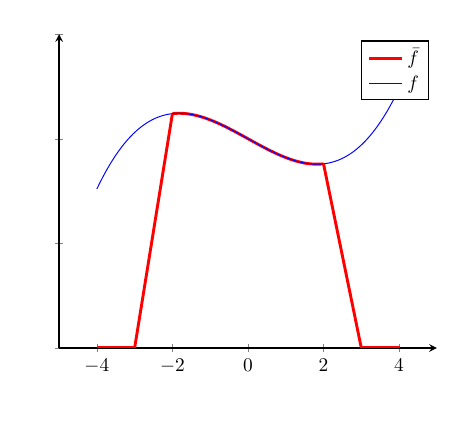
\begin{tikzpicture}[scale=0.7]
\begin{axis}[
    axis lines = left,
    xmin=-5,
    xmax=5,
    ymin=0,
    ymax=30,
    xlabel = $$,
    ylabel = {$$},
    yticklabels={,,}
]
%Below the red parabola is defined
\addplot [
    domain=-2:2, 
    samples=100, 
    line width=1.5,
    color=red,
]
{0.2*x^3 - 2*x + 20};
%Here the blue parabloa is defined
\addplot [
    domain=-4:4, 
    samples=100,         line width=0.5, 
    color=blue,
    ]
    {0.2*x^3 - 2*x + 20};
        \addlegendentry{$\bar f$}

\addplot [
    domain=3:4, 
    samples=100,
        line width=1.5, 
    color=red,
    ]
    {0};
\addplot [
    domain=-3:-2, 
    samples=100, 
    color=red,
       line width=1.5,
    ]
    {22.4*x+67.2};
    \addlegendentry{$f$}

\addplot [
    domain=-4:-3, 
    samples=100,
        line width=1.5, 
    color=red,
    ]
    {0};
    \addplot [
    domain=2:3, 
    samples=100, 
    color=red,
       line width=1.5,
    ]
    {-17.6*x+52.8};

\end{axis}
\end{tikzpicture}
		\end{center}
			  In Worten: $\bar f$ ist gleich $f$ in $[-k,k]$, null au\ss erhalb von $[-k-1,k+1]$ und verbindet dazwischen linear $0$ und $f(k)$ bzw. $f(-k)$. Die wichtige dazu gewonnene Information ist, dass $\bar f$ gleichm\"a\ss ig stetig ist. Das gilt, weil stetige Funktionen auf kompakten Mengen gleichm\"a\ss ig stetig sind (siehe Analysis 1). Jetzt kommt ein mehrfach genutzter Trick aus der Analysis. Wir addieren zwei Mal $0$ und nutzen die Dreicksungleichung
			 \begin{align}\label{F4}
				 \quad |\E[f(X_n)] - \E[f(X)]|
			 	\overset{\triangle}{\leq} \underbrace{\E[|f(X_n) - \bar f(X_n)|]}_{:= \text{ I}_n} + \underbrace{\E[|\bar f(X_n) - \bar f(X)|]}_{:= \text{ II}_n} + \underbrace{\E[|\bar f(X) - f(X)|]}_{:= \text{ III}_n}
			 \end{align}
			 und betrachten einzeln die Grenzwerte der drei Summanden. Aus (i), und weil $\bar f$ gleichmäßig stetig, wissen wir, dass $\text{II}_n \to 0$ f\"ur $n \to \infty$. F\"ur den dritten Summanden gilt
			 \begin{align*}
			 	\text{III}_n &= \E[|f(X) - \bar f(X)| \cdot (\mathbf 1_{[-k,k]}(X)+\mathbf{1}_{[-k,k]^C}(X))] \\
				&\leq 0+\E[2||f||_{\infty} \mathbf{1}_{[-k,k]^C}(X)]\\
			 	&= 2||f||_{\infty} \mathbb{P}(X \in [-k,k]^C)\\
				&= 2||f||_{\infty} \mathbb{P}(X \notin [-k,k])\\
				\overset{\text{Mon.}}&{\leq} 2||f||_{\infty} \mathbb{P}(X \notin [-k+1,k-1])
				< 2 || f ||_\infty \varepsilon,
			 \end{align*}
			 wegen der Wahl von $k$ und weil $f(x)-\bar f(x)=0$ f\"ur $x\in [-k,k]$. Schlie\ss lich noch der erste Summand. Wegen der angenommenen stochastischen Konvergenz gilt 
			 $$0\leq \mathbb P(X_n\notin [-k,k], X\in [-k+1,k-1])\leq \mathbb P(|X_n-X|>1)\rightarrow 0,\quad n\to\infty.$$ Damit zerlegen wir wie folgt:
			 \begin{align*}
			 	\quad \text{I}_n 
				&= \E[|f(X_n) - \bar f(X_n)|\cdot (\mathbf{1}_{[-k,k]}(X_n)+\mathbf{1}_{[-k,k]^C}(X_n)]\\
				&\leq 0+ \E[ 2||f||_\infty \mathbf 1_{[-k,k]^C}(X_n)]\\
				&=2|| f|| _\infty \mathbb P(X_n \notin [-k,k])\\
				&=2||f||_\infty \big( \mathbb P(X_n\notin [-k,k], X\in [-k+1,k-1])+\mathbb P(X_n\notin [-k,k],X\notin  [-k+1,k-1]) \big)\\
				&\leq 2||f||_\infty \big( \mathbb P(|X_n-X|\geq 1)+\mathbb P(X\notin [-k+1,k-1]) \big)\\
				&\leq 2||f||_\infty \big( \mathbb P(|X_n-X|\geq 1)+\varepsilon) \big).
			 \end{align*}
			Die rechte Seite konvergiert dann gegen $2||f||_\infty \varepsilon$. In der Rechnung haben wir viele kleine Eigenschaften benutzt, checkt es mal selber Zeile f\"ur Zeile: Monotonie und Linearit\"at von Erwartungswerten, dass Erwartungswerte von Indikatoren Wahrscheinlichkeiten sind (siehe Proposition \ref{rechenregeln}), sowie die $\sigma$-Additivit\"at und Monotonie von Ma\ss en. \smallskip			 
			 
			 Die drei einzelnen Betrachtungen zusammen ergeben wegen \eqref{F4}
			 
			  \[0\leq \limsup\limits_{n \to \infty} |\E[f(X_n)] - \E[f(X)]| \leq 2 ||f||_{\infty} \varepsilon + 0 + 2||f||_{\infty}\varepsilon. \] 
			 Weil $\varepsilon$ beliebig war, folgt daraus $\limsup\limits_{n \to \infty} |\E[f(X_n)] - \E[f(X)]|=0$ und damit $ \lim\limits_{n \to \infty} \E[f(X_n)] = \E[f(X)]$. Das ist die Konvergenz in Verteilung. \smallskip
			 
Die Hauptrichtungen sind nun vollst\"andig bewiesen. Wir zeigen jetzt noch, dass eine Umkehrung gilt, wenn der Grenzwert eine konstante Zufallsvariable ist:\smallskip

\textbf{Konvergenz in Verteilung gegen eine \underline{konstante} Zufallsvariable} $\Rightarrow$ \textbf{ Stochastische Konvergenz}:

Sei nun $(X_n)$ eine Folge von Zufallsvariablen, die gegen eine fast sicher konstante Zufallsvariable $X$ in Verteilung konvergiert. Sei $\eta\in\R$ der Wert, den $X$ $\mathbb P$-fast sicher annimmt und sei $\varepsilon>0$ beliebig. Sei nun $I=[\eta-\varepsilon, \eta+\varepsilon]$ und $f$ eine stetige Funktion mit $f\leq \mathbf 1_I$ sowie $f(\eta)=1$. Nat\"urlich gibt es so ein $f$, zum Beispiel das aus folgendem Bildchen:
\begin{center}



\tikzset{every picture/.style={line width=0.75pt}} %set default line width to 0.75pt        

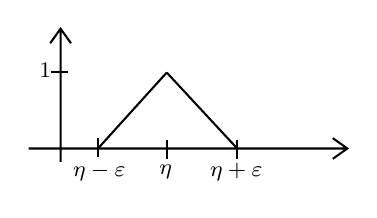
\begin{tikzpicture}[x=0.75pt,y=0.75pt,yscale=-1,xscale=1]
%uncomment if require: \path (0,300); %set diagram left start at 0, and has height of 300

%Shape: Axis 2D [id:dp6803750341520275] 
\draw  (266,150.59) -- (419.5,150.59)(281.35,92.88) -- (281.35,157) (412.5,145.59) -- (419.5,150.59) -- (412.5,155.59) (276.35,99.88) -- (281.35,92.88) -- (286.35,99.88)  ;
%Straight Lines [id:da7239111188912024] 
\draw    (332.5,114) -- (299,151) ;


%Straight Lines [id:da11710965322449962] 
\draw    (332.5,114) -- (366.83,151) ;


%Straight Lines [id:da1606239616323779] 
\draw    (284.95,113.75) -- (276.95,113.75) ;


%Straight Lines [id:da9124228840014664] 
\draw    (332.5,146.67) -- (332.5,155.67) ;


%Straight Lines [id:da9843095899175679] 
\draw    (366.5,146.67) -- (366.5,155.67) ;


%Straight Lines [id:da8761311329641914] 
\draw    (299.5,145.67) -- (299.5,154.67) ;



% Text Node
\draw (274,113) node  [font=\footnotesize] [align=left] {{\footnotesize 1}};
% Text Node
\draw (332,162) node   [align=left] {{\footnotesize $\eta$}};
% Text Node
\draw (366,162) node   [align=left] {{\footnotesize $\eta+\varepsilon$}};
% Text Node
\draw (300,162) node   [align=left] {{\footnotesize $\eta-\varepsilon$}};


\end{tikzpicture}
\end{center}
Wegen der angenommenen Konvergenz in Verteilung gilt damit
\begin{align*}
	1&=f(\eta)\\
	\overset{\ref{rechenregeln} \text{ (iii)}}&{=}\E[f(X)]\\
	&=\lim_{n\to\infty}\E[f(X_n)]\\
	\overset{\text{Monotonie}}&{\leq} \limsup_{n\to\infty} \E[\mathbf 1_{I}(X_n)]\\
	\overset{\ref{rechenregeln}\text{ (iv)}}&{=}\limsup_{n\to\infty} \mathbb P(X_n\in I)\leq 1,
\end{align*}
weil Wahrscheinlichkeiten immer durch $1$ dominiert sind. Weil obere und untere Schranke gleich sind, bekommen wir $\lim_{n\to\infty} \mathbb P(X_n\in I)=1$ und damit
\begin{align*}
	\mathbb P(|X_n-X|>\varepsilon)=\mathbb P(|X_n-\eta|>\varepsilon)=\mathbb P(X_n\notin I)=1-\mathbb P(X_n\in I)\to 0,\quad n\to\infty.
\end{align*}		
Warum tauchte gerade der Limes superior auf? Das liegt einfach nur daran, dass wir nicht wissen, ob der Grenzwert der Erwartungswerte existiert. Wir wissen das zwar f\"ur stetige Funktionen, aber der Indikator ist nicht stetig. \smallskip

\textbf{Stochastische Konvergenz } $\Rightarrow$ \textbf{ Fast sichere Konvergenz einer Teilfolge}:

Den Teil liefern wir nach dem Borel-Cantelli Lemma nach, siehe die Bemerkung \ref{bem4}.
%
%Wie immer gilt, dass man den Beweis genau anschauen sollte, wenn die Aussage nicht ganz klar ist. Wir nehmen an, dass die Folge $(X_n)$ stochastisch gegen $X$ konvergiert, f\"ur jedes $\varepsilon>0$ die Folge $a_n:=\mathbb P(|X_n-X|>\varepsilon)$ also eine Nullfolge ist. Wenn wir das mit Quantoren sauber ausschreiben, steht da also
%\begin{align}\label{sa}
%	\forall \varepsilon, \varepsilon'>0 \,\exists N\in \N: \mathbb P(|X_n-X|>\varepsilon)<\varepsilon', \quad \forall n\geq N.
%\end{align}
%Weil wir $\varepsilon$ und $\varepsilon'$ beliebig w\"ahlen d\"urfen, w\"ahlen wir $\varepsilon=\frac 1 k$ und $\varepsilon'=\frac{1}{2^k}$ f\"ur $k\in\N$. Wenn wir das zugeh\"orige $N$ aus \eqref{sa} als $n_k$ bezeichnen, so haben wir eine Teilfolge $X_{n_1}, X_{n_2}, ...$ gefunden, die folgendes Absch\"atzung erf\"ullt:
%\begin{align*}	
%	\mathbb P\Big(|X_{n_k}-X|>\frac 1 k\Big)<\frac{1}{2^k},\quad k\in\N.
%\end{align*}
%Um die fast sichere Konvergenz gerade dieser Teilfolge $X_{n_1}, X_{n_2}, ...$ gegen $X$ zu zeigen, nutzen wir folgende Beobachtung. Es gilt nat\"urlich
%\begin{align*}
%	\bigcap_{k=j}^\infty \Big\{\omega\in \Omega: |X_{n_k}(\omega)-X(\omega)|\leq\frac{1}{k} \Big\}\subseteq \big\{\omega\in \Omega: X_{n_k}(\omega) \to X(\omega)\big\}
%\end{align*}
%f\"ur alle $j\in\N$ oder alternativ, durch Komplementbildung und de Morgan, 
%\begin{align*}
%	\big\{\omega\in \Omega: X_{n_k}(\omega) \not\to X(\omega) \big\} \subseteq \bigcup_{k=j}^\infty \Big\{\omega\in \Omega: |X_{n_k}(\omega)-X(\omega)|>\frac{1}{k} \Big\}.
%\end{align*}
%Damit sind wir fertig: F\"ur $j\in\N$ beliebig gilt somit
%\begin{align*}
%	0&\leq \mathbb P(X_{n_k}\not \to X)\\
%	\overset{\text{Monotonie}}&{\leq}\mathbb P\Big(\bigcup_{k=j}^\infty\Big\{|X_{n_k}-X|>\frac{1}{k}\Big\}\Big)\\
%	\overset{\text{Subadd.}}&{\leq} \sum_{k=j}^\infty \mathbb P\Big(|X_{n_k}-X|>\frac 1 k \Big)\\
%	\overset{\text{Wahl der }n_k}&{\leq} \sum_{k=j}^\infty \frac{1}{2^k}.
%\end{align*}
%Weil $j$ beliebig war, k\"onnen wir auf der rechten Seite $j$ nach $+\infty$ schicken und damit gilt (die geometrische Reihe mit $q=\frac 1 2$ konvergiert) $0\leq \mathbb P(X_{n_k}\not \to X)\leq 0$ oder $\mathbb P(X_{n_k} \to X)=1$. Also konvergiert die Teilfolge $X_{n_1}, X_{n_2}, ...$ fast sicher gegen $X$.
\end{proof}

Aus dem Konvergenzdiagramm folgt nat\"urlich, dass fast sichere Konvergenz auch Konvergenz in Verteilung impliziert. \"Uberlegt doch mal, warum diese Aussage sehr viel schneller auch ohne den Umweg \"uber die stochastische Konvergenz folgt (Stichwort dominierte Konvergenz).\smallskip




	Das Ziel ist immer, die \enquote{starken} Konvergenzen (links im Bildchen) zu zeigen. Das geht leider nicht immer! Um die Begriffe mit Leben zu f\"ullen, zeigen wir drei ber\"uhmte S\"atze, je einen f\"ur stochastische Konvergenz, fast sichere Konvergenz und Konvergenz in Verteilung:
\begin{itemize}
	\item schwaches Gesetz der gro\ss en Zahlen (stochastische Konvergenz)
	\item starkes Gesetz der gro\ss en Zahlen (fast sichere Konvergenz)
	\item Zentraler Grenzwertsatz (Konvergenz in Verteilung)
\end{itemize}
Beim schwachen Gesetz der gro\ss en Zahlen werden wir merken, dass Konvergenz in $\mathcal L^p$ gerade f\"ur $p=1$ oder $p=2$ ein extrem n\"utzliches Werkzeug ist. Der Grund ist, dass man mit Momenten gut rumrechnen kann (Ausmultiplizieren, Linearit\"at, ...). Folgendes Resultat ist nicht sehr kompliziert, kann aber schon n\"utzlich sein. Sehr viel n\"utzlicher wird n\"achste Woche aber das starke Gesetzt der gro\ss en Zahlen sein!

\begin{satz}\label{schwaches}
\link{https://www.youtube.com/watch?v=e-i3vo2epBI&list=PLy5qRKPWp6SBwfc1kn-b66cWc84cOgvqZ&index=26&t=6815s} \textbf{[Schwaches Gesetz der großen Zahlen]}
	\begin{enumerate}[label=(\roman*)]
		\item Klassische Variante: Sind $X_1,X_2,...$ u.i.v. mit $\E[X_1^2] < \infty$, so gilt
		\[ \frac{1}{n} \sum_{k=1}^{n} X_k \overset{P}{\longrightarrow} \E[X_1], \quad n \to \infty. \]
		\item Variante mit schw\"acheren Annahmen: Sind $X_1,X_2,...$ quadratintegrierbar, paarweise unkorreliert (z. B. paarweise unabh\"angig) mit identischen Erwartungswert und
		\begin{align}
		 \frac{1}{n^2} \sum\limits_{k=1}^{n} \V(X_k) \to 0,\quad n\to\infty, \label{F1}
		\end{align}
		so gilt
		\[ \frac{1}{n} \sum_{k=1}^{n} X_k \overset{P}{\longrightarrow} \E[X_1], \quad n \to \infty. \]
	\end{enumerate}
\end{satz}
F\"urs bessere Verst\"andniss kann man \"uberlegen, wie die Annahme \enquote{identischer Erwartunswert} in (ii) ersetzt werden kann, da gibt es verschiedene M\"oglichkeiten. 
\begin{proof}
	(i)  Wenn man den Beweis gesehen hat, ist alles ziemlich simple: \textbf{Erst Tschebycheff, dann Bienaym\'e}. Mit Tschebycheff und Bienaym\'e gilt f\"ur beliebiges $\varepsilon>0$ aufgrund der u.i.v. Annahme
	\begin{align*}
		\mathbb{P}\Big(\Big|\frac{1}{n} \sum\limits_{k=1}^{n} X_k-\E[X_1]\Big| \geq \varepsilon\Big)
		&=\mathbb{P}\Big(\Big| \sum\limits_{k=1}^{n} X_k-n\E[X_1)\Big| \geq n \varepsilon\Big)\\
		\overset{\ref{Markov}}&{\leq} \frac{\V \big[\sum_{k=1}^n X_k\big] }{n^2\varepsilon^2}\\
		\overset{\ref{bien}}&{=} \frac{\sum\limits_{k=1}^{n} \V[X_k]}{n^2 \varepsilon^2}\\
		& = \frac{n \cdot \V[X_1]}{n^2 \varepsilon^2} \to 0, \quad n \to \infty.
		\end{align*}
		Also gilt $\frac{1}{n}\sum_{k=1}^n X_k\overset{P}{\rightarrow} \E[X_1]$ f\"ur $n\to\infty$. Beachtet dabei, dass wir f\"ur Tschebycheff $\E[\sum_{k=1}^n X_k]=n\E[X_1]$ genutzt haben. Um ganz genau zu sein (und wir wollen nat\"urlich genau sein!), merken wir noch an, dass \enquote{$>$} oder \enquote{$\geq$} in der Definition der schwachen Konvergenz nat\"urlich keine Rolle spielt, $\varepsilon$ ist schlie\ss lich beliebig.\smallskip
		
		Man kann das Argument auch anders hinschreiben. Benutzt zum \"Uben doch mal statt Tschebycheff die Markov Ungleichung mit $h(x)=x^2$ plus die Verschiebungsformel f\"ur die Varianz.\smallskip
				
		(ii) Um die schw\"acheren Annahmen von (ii) zu verstehen, brauchen wir nur in den vier Zeilen des Arguments zu schauen, wie wir die Unabh\"angigkeit abschw\"achen k\"onnen, so dass die Konvergenz immer noch folgt. Wir sehen dann sofort, dass f\"ur Bienaym\'e nur paarweise unkorreliert gebraucht wird, dann aber f\"ur die Konvergenz noch \eqref{F1} gefordert werden muss (es wird nicht mehr identisch verteilt angenommen, es gilt also nicht $\V[X_k]=\V[X_1]$). Schaut euch das in Ruhe an, um die Idee \enquote{erst Tschebyscheff, dann Bienaym\'e} einzubrennen.
\end{proof}

	Zum besseren Verst\"andnis kann man mal ausprobieren, ob man das schwache Gesetz genauso mit der Annahme $\E[|X_1|]<\infty$ beweisen k\"onnte. Warum funktioniert der Beweis nicht, wenn man die Markovungleichung f\"ur das erste Moment statt f\"ur das zweite Moment ausprobiert? Der Trick an dem Beweis mit zweiten Momenten ist, dass die Varianz der Summe, die eigentlich aus $n^2$ vielen Summanden besteht, sich aufgrund der Annahme (unabh\"angig oder unkorreliert) zu einer Summe aus nur $n$ vielen Summanden reduziert (im Beweis von Bienaym\'e k\"urzen sich die meisten Terme raus). Damit dominiert der Nenner mit $n^2$ und die obere Schranke konvergiert gegen $0$. Der Effekt passiert beim ersten Moment nicht, weil keine \enquote{gemischten Terme} $\E[X_iX_j]=0$ auftauchen. Deshalb st\"unde sowohl in Z\"ahler als auch in Nenner etwas mit $n$, die obere Schranke w\"urde also nicht gegen $0$ konvergieren, in Formeln (f\"ur $\E[X_1]=0$):
	\begin{align*}
		\mathbb{P}\Big(\Big|\frac{1}{n} \sum\limits_{k=1}^{n} X_k\Big| \geq \varepsilon\Big)
		&\overset{\ref{Markov},\, h(x)=|x|}{\leq} \frac{\E \big[\big|\sum_{k=1}^n X_k\big|\big] }{n\varepsilon}\leq \frac{\sum_{k=1}^n \E[|X_k|]}{n\varepsilon}= \frac{n\E[|X_1|]}{n\varepsilon} \not\to 0,
	\end{align*}
	f\"ur $n\to\infty$. Genau den selben Effekt werden wir beim Beweis des starken Gesetzes der gro\ss en Zahlen sehen, bei dem wir endliche 4.te Momente annehmen und bei der Markovungleichung mit $h(x)=x^4$ genug Summanden verschwinden, dass der Nenner dominiert.
	
	
%\begin{bem}
%	Gilt $\E[X_2] < \infty$, so gilt $\V(X) = \V(X+a)$. Warum? $\V(X+a) = \E[(X+a -\E[X+a])^2] = \E[(X+a -(\E[X]+\E[a]))^2] = \E[(X -\E[X])^2] = \V(X)$.
%\end{bem}

%\begin{proof}
%	\OE \space gelte $\E[X_1] = 0$. Warum? Wenn nicht, betrachte $Y_n = X_n - \E[X_n]$ (das nennt man zentrieren). Damit gilt 
%	\begin{gather*}
%		\mathbb{P}\Big(\Big|\frac{1}{n} \sum\limits_{i=1}^{n} (X_i - \E[X_1]) - 0\Big| > \varepsilon\Big) = \mathbb{P}\Big(\Big|\frac{1}{n} \sum\limits_{i=1}^{n} (X_i - \E[X_i]) - 0\Big| > \varepsilon\Big) \\
%		= \mathbb{P}\Big(\Big|\frac{1}{n} \sum\limits_{i=1}^{n} Y_i - 0\Big| > \varepsilon\Big) \to 0, \: n \to \infty,
%	\end{gather*}
%	weil $\E[Y_i] = \E[X_i - \E[X_i]] = \E[X_i] - \E[X_i] = 0$.
%	Sei also $\E[X_1] = 0$. 
%	\begin{gather*}
%		\mathbb{P}\Big(\Big|\frac{1}{n} \sum\limits_{i=1}^{n} X_i - 0\Big| > \varepsilon\Big) = \mathbb{P}\Big(\Big|\frac{1}{n} \sum\limits_{i=1}^{n} X_i - \E[\frac{1}{n} \sum\limits_{i=1}^{n} X_i]\Big| > \varepsilon\Big) \\
%		\overset{\text{\ref{tscheby}}}{\leq} \frac{\V\Big(\frac{1}{n} \sum\limits_{i=1}^{n} X_i\Big)}{\varepsilon^2} = \frac{\frac{1}{n^2} \V\Big(\sum\limits_{i=1}^{n} X_i\Big)}{\varepsilon^2} \overset{\text{\ref{bien}}}{=} \frac{\frac{1}{n^2} \sum\limits_{i=1}^{n} \V\Big(X_i\Big)}{\varepsilon^2}  \\
%		= \frac{\frac{1}{n^2} \cdot n \cdot \sum\limits_{i=1}^{n} \V\Big(X_i\Big)}{\varepsilon^2} = \frac{\sum\limits_{i=1}^{n} \V\Big(X_i\Big)}{n \varepsilon^2} \to 0, \: n \to \infty.
%	\end{gather*}
%\end{proof}


\section{Starkes Gesetz der großen Zahlen}\label{sec:GGZ} \marginpar{\textcolor{red}{Vorlesung 26}}
	Was bedeutet die stochastische Konvergenz, bzw. warum ist sie schwach? Seien als Beispiel $X_1,X_2,...$ u.i.v. Würfel, also diskret gleichverteilt auf $\{1,...,6\}$. Wegen $\E[X_1]=3,5$ bedeutet das schwache Gesetz der großen Zahlen (w\"ahle zum Beispiel $\varepsilon=0.01$), dass 
	\[ \mathbb{P}\Big(3,49 < \frac{1}{n} \sum\limits_{i=1}^{n} X_i < 3,51\Big) = \mathbb{P}\Big(\Big|\frac 1 n\sum\limits_{i=1}^{n} X_i - \E[X_1]\Big| < 0,01\Big) \to 1, \quad n \to \infty. \]
	In Worten steht hier: \enquote{Der Mittelwert wird mit hoher Wahrscheinlichkeit nah bei 3,5 liegen, wenn $n$ groß ist.} Es wird damit nicht ausgeschlossen, dass der Mittelwert mit kleiner Wahrscheinlichkeit weit vom Erwartungswert entfernt liegt. Genau hier liegt der Unterschied zum starken Gesetz der gro\ss en Zahlen, das wir als n\"achstes beweisen wollen. Hier wird die stochastische Konvergenz durch fast sichere Konvergenz ersetzt. Weil in der Definition der fast sicheren Konvergenz alle $n$ gemeinsam \textit{innerhalb} der Wahrscheinlichkeit auftauchen, $\mathbb P(X_n\to X)=1$, kann der Effekt nicht auftreten.\smallskip

	
Als Hilfsmittel f\"ur den Beweis diskutieren wir zun\"achst das Borel-Cantelli Lemma. Dazu zun\"achst ein paar Definitionen:	
\begin{deff}
\link{https://www.youtube.com/watch?v=AfWbQxemkRI&list=PLy5qRKPWp6SBwfc1kn-b66cWc84cOgvqZ&index=27&t=235s}
	Sei $(\Omega, \cA, \mathbb{P})$ ein Wahrscheinlichkeitsraum und seien $A_1,A_2,... \in \cA$ beliebige Ereignisse.
	\begin{enumerate}[label=(\roman*)]
		\item \begin{align*}
			\limsup\limits_{n \to \infty} A_n 
			&:= \bigcap_{n=1}^{\infty} \bigcup_{k=n}^{\infty} A_k\\
			&= \{ \omega \in \Omega\colon \omega \in A_n \text{ für unendlich viele } n \}\\ 
			\overset{\text{Notation}}&{=} \{ A_n \text{ unendlich oft} \} 
		\end{align*}
		heißt \textbf{Limes superior} der Folge $(A_n)$ von Ereignissen.
		\item \begin{align*}
			\liminf\limits_{n \to \infty} A_n 
			&:= \bigcup_{n=1}^{\infty} \bigcap_{k=n}^{\infty} A_k\\
			&= \{ \omega \in \Omega\colon \omega \in A_n \text{ schließlich immer} \}\\
			\overset{\text{Notation}}&{=} \{ A_n \text{ schließlich immer} \}
		\end{align*}
		\textbf{Limes inferior} der Folge $(A_n)$ von Ereignissen.
	\end{enumerate}
\end{deff}
Weil aufgrund der Definition einer $\sigma$-Algebra abz\"ahlbare Schnitte und Vereinigungen wieder in $\mathcal A$ sind, sind auch $\limsup_{n\to\infty} A_n$ und $\liminf_{n\to\infty} A_n$ in $\mathcal A$. Wem der Begriff \enquote{schlie\ss lich immer} suspekt ist, der oder die schaue einfach die formelle Definition an. Diese besagt, dass es eine nat\"urliche Zahl $n$ gibt, so dass das Ereigniss danach \textit{immer} eintritt (der Durchschnitt von Mengen enth\"alt alle Elemente, die in allen Mengen enthalten sind).\smallskip

Tats\"achlich haben die neuen Begriffe $\liminf$ und $\limsup$ f\"ur Mengen auch etwas mit den uns bekannten Begriffen $\liminf$ und $\limsup$ f\"ur Folgen zu tun:
\begin{lemma}
\link{https://www.youtube.com/watch?v=AfWbQxemkRI&list=PLy5qRKPWp6SBwfc1kn-b66cWc84cOgvqZ&index=27&t=579s}
	Sei $(\Omega, \cA, \mathbb{P})$ ein Wahrscheinlichkeitsraum und seien $A_1,A_2,... \in \cA$ beliebige Ereignisse. Dann gelten:
	\begin{enumerate}[label=(\roman*)]
		\item $ \liminf\limits_{n \to \infty} A_n \subseteq \limsup\limits_{n \to \infty} A_n,$
		\item $(\liminf\limits_{n \to \infty} A_n)^C = \limsup\limits_{n \to \infty} A_n^C,$
		\item $\limsup\limits_{n \to \infty} \mathbf{1}_{A_n}(\omega) = \mathbf{1}_{\limsup\limits_{n \to \infty} A_n}(\omega),\quad \forall \omega \in \Omega,$
		\item $\liminf\limits_{n \to \infty} \mathbf{1}_{A_n}(\omega) = \mathbf{1}_{\liminf\limits_{n \to \infty} A_n}(\omega),\quad \forall \omega \in \Omega.$
	\end{enumerate}
\end{lemma}

\begin{proof}
	Denkt einfach mal kurz dar\"uber nach, was $\liminf_{n\to\infty} a_n=1$ oder $\liminf_{n\to\infty} a_n=0$ f\"ur eine reelle Folge $(a_n)$ bedeutet, wenn diese nur die Werte $0$ und $1$ annimmt. \"Ubung.
\end{proof}

Das Borel-Cantelli Lemma gibt uns gleich ein Kriterium, ob die Wahrscheinlichkkeit des $\limsup A_n$ null ist oder (mit einer st\"arkeren Annahme) $1$ ist. Daf\"ur basteln wir mit Zufallsvariablen rum, alles basiert auf folgender Bemerkung:
\begin{bem}\label{ereig}
\link{https://www.youtube.com/watch?v=AfWbQxemkRI&list=PLy5qRKPWp6SBwfc1kn-b66cWc84cOgvqZ&index=27&t=915s}
	Sei $(\Omega, \cA, \mathbb{P})$ ein Wahrscheinlichkeitsraum und seien $A_1,A_2,... \in \cA$ beliebige Ereignisse. Dann gilt
	\begin{align*}
		A_1, A_2, ... \text{ sind unabh\"angig}\quad \Leftrightarrow\quad  \mathbf{1}_{A_1},\mathbf{1}_{A_2},... \text{ sind unabhängig},
	\end{align*}	
	wobei wir auch die Unabh\"angigkeit durch paarweise Unabh\"angigkeit ersetzten k\"onnen.
	Beachte: $A_1, A_2, ...$ ist ein Folge von Ereignissen, wohingegen $\mathbf{1}_{A_1},\mathbf{1}_{A_2},... $ eine Folge von Zufallsvariablen ist. Das ist also ein guter Moment, in Kapitel \ref{Sunab} die Definitionen von Unabh\"angigkeit von Ereignissen und Zufallsvariablen nochmal zu vergleichen! Warum gilt die \"Aquivalenz? Checken wir die Definitionen:
	\begin{align*}
		\mathbf{1}_{A_1},\mathbf{1}_{A_2},... \text{ unabh\"angig}\quad 
		\overset{\text{Def. }\ref{unab}}&{\Leftrightarrow} \quad \sigma(\mathbf{1}_{A_1}),\sigma(\mathbf{1}_{A_2}),... \text{ unabhängig}\\
		\overset{\ref{yu}}&{\Leftrightarrow}\quad \{ \emptyset, \Omega, A_1, A_1^C \},\{ \emptyset, \Omega, A_2, A_2^C \}, ... \text{ unabhängig}\\
		&\Leftrightarrow\quad A_1, A_2, ... \text{ unabh\"angig}.
	\end{align*}
F\"ur die dritte \"Aquivalenz haben wir Definition \ref{Ka} genutzt, sowie die Eigenschaft, dass Unabh\"angigkeit von Ereignissen sich auch auf die Komplemente \"ubertr\"agt (\"Ubung). 
	
	
\end{bem}

\begin{satz}\label{BC}
\link{https://www.youtube.com/watch?v=AfWbQxemkRI&list=PLy5qRKPWp6SBwfc1kn-b66cWc84cOgvqZ&index=27&t=1127s} \textbf{[Borel-Cantelli Lemma]}
	Sei $(\Omega, \cA, \mathbb{P})$ ein Wahrscheinlichkeitsraum und seien $A_1,A_2,... \in \cA$ beliebige Ereignisse, so gelten:
	\begin{enumerate}[label=(\roman*)]
		\item \[ \sum\limits_{n = 1}^{\infty} \mathbb{P}(A_n) < \infty \quad \Rightarrow\quad  \mathbb{P}\big(\limsup\limits_{n \to \infty} A_n\big) =0. \]
		\item Sind die $A_1, A_2, ...$ \textit{zusätzlich} paarweise unabhängig, so gilt \[ \sum\limits_{n = 1}^{\infty} \mathbb{P}(A_n) = \infty \quad \Rightarrow \quad \mathbb{P}\big(\limsup\limits_{n \to \infty} A_n\big) = 1. \]
	\end{enumerate}
\end{satz}
	Damit kennt ihr nun euer erstes \enquote{0-1-Gesetz}: Sind die Ereignisse $A_1, A_2, ...$ paarweise unabh\"angig, so gilt automatisch $\mathbb P(\limsup_{n\to\infty} A_n)\in \{0,1\}$ und
	\begin{align*}
		\mathbb P(\limsup_{n\to\infty}A_n)=1\quad \Longleftrightarrow \quad\mathbb P(\limsup_{n\to\infty}A_n)>0\quad \Longleftrightarrow \quad  \sum_{n=1}^\infty \mathbb P(A_n)=\infty.
	\end{align*}
	 Das n\"utzliche an 0-1-Gesetzen ist, dass man nur zeigen muss, dass etwas strikt positive Wahrscheinlichkeit hat, um sogar Wahrscheinlichkeit $1$ zu schlie\ss en. 

\begin{proof}\abs
	\begin{enumerate}[label=(\roman*)]
		\item \enquote{triviale Rechnung}: Die einfache Richtung folgt aus einfachen Manipulationen mit Mengen und Eigenschaften von Ma\ss en:
		\begin{align*}
			\mathbb{P}(\limsup\limits_{n \to \infty} A_n) 
			&= \mathbb{P}\Big(\bigcap_{n=1}^{\infty} \bigcup_{k=n}^{\infty} A_k\Big)\\
			\overset{\text{Stet. Ma\ss e}}&{=}\lim\limits_{N \to \infty} \mathbb{P}\Big(\bigcap_{n=1}^{N} \bigcup_{k=n}^{\infty} A_k\Big)\\
			\overset{\text{Monotonie}}&{\leq}\lim\limits_{N \to \infty} \mathbb{P}\Big(\bigcup_{k=N}^{\infty} A_k\Big) \\
			\overset{\text{Subadd.}}&{\leq} \lim\limits_{N \to \infty} \sum\limits_{k=N}^{\infty} \mathbb{P}(A_k) = 0.
		\end{align*}
		Die letzte Gleichheit gilt nach Annahme und Analysis 1 (Eigenschaft konvergenter Reihen), weil $\sum_{k=1}^\infty \mathbb P(A_k)<\infty$ angenommen wurde.
		\item Die R\"uckrichtung ist deutlich schwieriger, wir nutzen die sogenannte \enquote{zweite-Momente-Methode}. Daf\"ur werden erstes und zweites Moment einer geeigneten Zufallsvariable miteinander verglichen. Wir betrachten im Folgenden die Zufallsvariablen $\mathbf 1_{A_n}$, die aufgrund von Bemerkung \ref{ereig} unabh\"angig sind. Weil die Zufallsvariablen nur die Werte $0$ und $1$ annehmen, sind sie Bernoulli-verteilt. Genauer, es gilt $\mathbf 1_{A_n}\sim \operatorname{Ber}(p_n)$, wobei $p_n=\mathbb P(A_n)$ die Wahrscheinlichkeit f\"ur den Wert $1$ ist. Kleine Erinnerung: F\"ur $\operatorname{Ber}(p)$-verteilte Zufallsvariablen ist der Erwartungswert $p$ und die Varianz $p(1-p)$. Das werden wir im Folgenden ausnutzen.\smallskip
		
		Wir betrachten die Folge
		\[ Z_k = \sum\limits_{n=1}^{k} \mathbf{1}_{A_n},\quad k\in\N, \]
		weil mit dieser Folge $\limsup_{n\to\infty} A_n$ beschrieben werden kann:
		\begin{align}\label{kyp}
			\omega \in \limsup\limits_{n \to \infty} A_n \quad \Leftrightarrow \quad +\infty=\sum\limits_{n=1}^{\infty} \mathbf{1}_{A_n}(\omega) = \lim\limits_{k \to \infty} Z_k(\omega).
		\end{align}
		Das gilt nat\"urlich weil die Reihe nur aus Summanden $0$ oder $1$ besteht und daher unendlich ist genau dann, wenn unendlich viele Summanden $1$ sind, also wenn $\omega$ in unendlich vielen $A_n$ ist. F\"ur Erwartungswert und Varianz gelten
		 \begin{align*}
		 	\E[Z_k] &= \sum\limits_{n=1}^{k} \E[\mathbf{1}_{A_n}] = \sum\limits_{n=1}^{k} \mathbb P(A_n) \overset{\text{Ann.}}{\longrightarrow}+\infty, \quad k \to \infty,
		\end{align*}
		sowie
		\begin{align*}
		 	\V[Z_k] \underset{\text{\ref{ereig}}}&{\overset{\text{\ref{bien}}}{=}} \sum\limits_{n=1}^{k}\V[\mathbf{1}_{A_n}]
		 	= \sum\limits_{n=1}^{k} \mathbb P(A_n)(1-\mathbb P(A_n)) \leq \sum\limits_{n=1}^{k} \mathbb P(A_n) = \E[Z_k],
		 \end{align*}
		 weil unabh\"angige Zufallsvariablen auch unkorrelliert sind. Jetzt benutzen wir Tschebyscheff mit den Formeln f\"ur Erwartungswert und Varianz:
		  \begin{align}\label{absch}
		 	\mathbb{P}\Big(|Z_k - \E[Z_k]| \geq \frac{\E[Z_k]}{2}\Big) \overset{\ref{Markov}}{\leq}\frac{\V[Z_k]}{\frac{1}{4} \E[Z_k]^2} \leq \frac{4\E[Z_k]}{\E[Z_k]^2} = \frac{4}{\E[Z_k]} \to 0,
		 \end{align}
		 f\"ur $k\to\infty$. Sei nun $\lambda > 0$ beliebig. Dann existiert wegen der Divergenz der Erwartungswerte gegen unendlich ein $k_0 \in \N$ mit $\frac{\lambda}{\E[Z_k]} < \frac{1}{2}$ f\"ur alle $k\geq k_0$.
		 Weil aufgrund der Definition von $Z_k$ auch $Z_k \leq \sum\limits_{n=1}^{\infty} \mathbf{1}_{A_n}$ gilt, bekommen wir für beliebiges $k \geq k_0$
		 \begin{align*}
		 	\mathbb{P}\Big(\sum\limits_{n=1}^{\infty} \mathbf{1}_{A_n} < \lambda \Big)& \leq \mathbb{P}(Z_k < \lambda)\\
			& = \mathbb{P}\Big(\frac{Z_k}{\E[Z_k]} < \frac{\lambda}{\E[Z_k]}\Big)\\
			& \leq \mathbb{P}\Big(\frac{Z_k}{\E[Z_k]} < \frac{1}{2}\Big)\\ 
		 	&= \mathbb{P}\Big(\frac{Z_k}{\E[Z_k]} - 1 < -\frac{1}{2}\Big)\\
			& \leq \mathbb{P}\Big(\Big|\frac{Z_k}{\E[Z_k]} - 1\Big| \geq \frac{1}{2}\Big)\\
		 	\overset{\text{Vor.}}&{=} \mathbb{P}\Big(\big|Z_k - \E[Z_k]\big| \geq \frac{\E[Z_k]}{2}\Big) \overset{\text{\eqref{absch}}}{\longrightarrow} 0, \quad k \to \infty.
		 \end{align*}
		Also gilt $\mathbb{P}\big(\sum\limits_{n=1}^{\infty} \mathbf{1}_{A_n} < \lambda \big)=0$. Weil $\lambda$ beliebig gew\"ahlt war, folgt aufgrund der Stetigkeit von Ma\ss en auch $\mathbb{P}\big(\sum\limits_{n=1}^{\infty} \mathbf{1}_{A_n} < \infty \big)=\lim_{N\to\infty}\mathbb{P}\big(\sum\limits_{n=1}^{\infty} \mathbf{1}_{A_n} < N \big) =0$. Wegen \eqref{kyp} gilt nun \[ \mathbb{P}\big(\limsup\limits_{n \to \infty}A_n\big) = \mathbb{P}\Big(\sum\limits_{n=1}^{\infty} \mathbf{1}_{A_n} = +\infty\Big) = 1. \]
	\end{enumerate}
\end{proof}
Kleine Anmerkung an dieser Stelle: Wenn im zweiten Teil statt paarweiser Unabh\"angigkeit sogar Unabh\"angigkeit angenommen wird, dann gibt es einen einfacheren Beweis f\"ur Teil (ii):
\begin{align*}
	\mathbb P\big((\limsup\limits_{n \to \infty} A_n)^C\big)	\overset{\text{de Morgan}}&= \mathbb{P}\Big(\bigcup_{n=1}^{\infty} \bigcap_{k=n}^{\infty} A^C_k\Big)\\
	\overset{\text{Subadd.}}&\leq \sum_{n=1}^\infty \mathbb{P}\Big(\bigcap_{k=n}^{\infty} A^C_k\Big)\\
		\overset{\text{Stet. Ma\ss e}}&\leq \sum_{n=1}^\infty \lim_{N\to\infty} \mathbb{P}\Big(\bigcap_{k=n}^NA^C_k\Big)\\
		\overset{\text{Unab.}}&= \sum_{n=1}^\infty \lim_{N\to\infty} \prod_{k=n}^N (1-\mathbb{P}(A_n))\\
		\overset{1-x\leq e^{-x}}&\leq \sum_{n=1}^\infty \lim_{N\to\infty} \prod_{k=n}^N e^{-\mathbb{P}(A_n)}\\
		&= \sum_{n=1}^\infty \lim_{N\to\infty}  e^{-\sum_{k=n}^N\mathbb{P}(A_n)}
		\overset{\text{Vor.}}{=}\sum_{n=1}^\infty \,0=0.
\end{align*}
Checkt mal genau, warum dieser Beweis Unabh\"angigkeit statt nur paarweise Unabh\"angigkeit benutzt! Die komplizierte Variante wurde haupts\"achlich aus didaktischen Gr\"unden gew\"ahlt, um Argumente mit der Markovungleichung und Bernoulli-Zufallsvariablen zu wiederholen.\smallskip

Nach diesem sehr abstrakten Highlight, nun zur\"uck zur fast sicheren Konvergenz und dem starken Gesetz der gro\ss en Zahlen. 
\begin{korollar}\label{ko}
\link{https://www.youtube.com/watch?v=AfWbQxemkRI&list=PLy5qRKPWp6SBwfc1kn-b66cWc84cOgvqZ&index=27&t=3005s}
	Seien $X, X_1, X_2, ...$ Zufallsvariablen auf einem Wahrscheinlichkeitsraum $(\Omega, \mathcal A, \mathbb P)$, dann gelten:
	\begin{enumerate}[label=(\roman*)]
		\item $$\sum_{n=1}^\infty \mathbb P(|X_n-X|>\varepsilon)<\infty\text{  f\"ur alle }\varepsilon>0 \quad\Longrightarrow\quad X_n\overset{\text{f.s.}}{\to}X,\quad n\to\infty.$$
		\item Unter der zus\"atzlich Annahme $X_1-X, X_2-X, ...$ sind paarweise unabh\"angig, gilt: $$\sum_{n=1}^\infty \mathbb P(|X_n-X|>\varepsilon)=+\infty\text{ f\"ur ein }\varepsilon>0\quad \Longrightarrow\quad X_n\overset{\text{f.s.}}{\not\to}X, \quad n\to\infty.$$
	\end{enumerate}
\end{korollar}
\begin{proof}
	Beide Aussagen folgen sofort aus Borel-Cantelli:
\begin{enumerate}[label=(\roman*)]
\item Mit $\varepsilon=\frac 1 k$ impliziert das Borel-Cantelli-Lemma $\mathbb P(|X_n-X|>\frac 1 k\text{ unendlich oft})=0$ bzw. $\mathbb P(|X_n-X|>\frac 1 k\text{ nur endlich oft})=1$ f\"ur alle $k\in\N$. Daraus folgt
	\begin{align*}
		\mathbb P(X_n\to X)&=\mathbb P\Big(\Big\{\omega: \forall k \in \N\, \exists N\in \N: |X_n(\omega)-X(\omega)|\leq \frac{1}{k}\, \forall n\geq N\Big\}\Big)\\
		&=\mathbb P\Big(\bigcap_{k=1}^\infty \Big\{\omega:  \exists N\in \N: |X_n(\omega)-X(\omega)|\leq \frac{1}{k}\, \forall n\geq N\Big\}\Big)\\
		&=\mathbb P\Big(  \Big\{\omega: |X_n(\omega)-X(\omega)|>\frac{1}{k}\text{ endlich oft}\Big\}\Big)=1,
	\end{align*}
	weil der Durchschnitt abz\"ahlbar vieler Mengen von Ma\ss{} $1$ auch Ma\ss{} $1$ hat (wegen Komplementbildung, abz\"ahlbare Vereinigungen von Nullmengen sind Nullmengen). Denkt an dieser Stelle nochmal daran, dass wir manchmal in Wahrscheinlichkeiten die $\omega$ bei Zufallsvariablen weglassen weil es sich besser liest.	
\item Borel-Cantelli impliziert $\mathbb P(|X_n-X|>\varepsilon\text{ unendlich oft})=1$, also ist die Wahrscheinlichkeit, dass $X_n$ gegen $X$ konvergiert, sogar $0$.
\end{enumerate}
\end{proof}

Wegen Borel-Cantelli k\"onnen wir den Unterschied von stochastischer und fast sicherer Konvergenz nun besser verstehen:
\begin{bem}\label{bem4}
\link{https://www.youtube.com/watch?v=AfWbQxemkRI&list=PLy5qRKPWp6SBwfc1kn-b66cWc84cOgvqZ&index=27&t=3657s} \textbf{[Stochastische Konvergenz vs. fast sichere Konvergenz]}
\begin{itemize}
\item	Um stochastische Konvergenz zu zeigen, muss $a_n:=\mathbb P(|X_n-X|>\varepsilon)$ f\"ur beliebiges $\varepsilon>0$  eine Nullfolge sein. Konvergiert die Nullfolge so schnell gegen $0$, dass auch der Reihengrenzwert $\sum_{n=1}^\infty a_n$ endlich ist, so konvergiert nach Korollar \ref{ko} die Folge $(X_n)$ fast sicher gegen $X$. Wenn wir uns an Analysis 1 erinnern, ist es ein gro\ss er Unterschied, ob die Reihe \"uber eine Folge konvergiert oder die Folge eine Nullfolge ist. Beispielsweise reicht f\"ur stochastische Konvergenz die Absch\"atzung $\mathbb P(|X_n-X|>\varepsilon)\leq \frac{1}{n}$ f\"ur fast sichere Konvergenz nicht!
	\item Wir m\"ussen noch einen Teil des Beweises von Satz 4.5.11 nachliefern. Das folgt aus dem ersten Teil des Korollars mit der Wahl der Teilfolge $n_k$, die $$\mathbb P\Big(|X_{n_k}-X|>\frac 1 k\Big)<\frac{1}{2^k}$$ erf\"ullt.
\end{itemize}
\end{bem}




\begin{beispiel}
\link{https://www.youtube.com/watch?v=AfWbQxemkRI&list=PLy5qRKPWp6SBwfc1kn-b66cWc84cOgvqZ&index=27&t=4036s}
Schauen wir uns das Beispiel \ref{Adam} nochmal etwas allgemeiner an, um ein konkretes Beispiel f\"ur Korollar \ref{ko} zu haben: Seien $X_1, X_2, ... $ unabh\"angige Zufallsvariablen mit $$\mathbb{P}(X_n = 1) = \frac{1}{n^p}, \quad \mathbb{P}(X_n = 0) = 1 - \frac{1}{n^p},$$ also $X_n \sim \operatorname{Ber}(\frac{1}{n^p})$, $n \in \N$. Man stelle sich wieder unabh\"angige Versuche vor ($1$ bedeutet \enquote{Erfolg}, $0$ bedeutet \enquote{Misserfolg}), bei denen die Wahrscheinlichkeit f\"ur \enquote{Erfolg} immer kleiner wird. Fragen wir uns wieder: Konvergiert die Folge fast sicher gegen die Zufallsvariable $X=0$? Wegen der angenommenen Unabh\"angigkeit gilt mit Korollar \ref{ko} 
\begin{align*}
	X_n\overset{\text{f.s.}}{\to} 0,\quad n\to\infty \quad &\Leftrightarrow\quad \sum_{n=1}^\infty \mathbb P(X_n=1)=\sum_{n=1}^\infty \frac{1}{n^p}<+\infty\quad
	\Leftrightarrow\quad p>1.
\end{align*}
Ausformuliert ist die Aussage noch spektakul\"arer weil die Konvergenz gegen $0$ einer Folge mit Werten $0$ oder $1$ bedeutet, dass die Folge irgendwann nur noch den Wert $0$ annimmt. Ist $p\leq 1$, so ist der Versuch also immer mal wieder erfolgreich, wohingegen f\"ur $p>1$ der Versuch nur endlich oft erfolgreich ist. Wenn man bedenkt, dass der Versuch unendlich oft ausgef\"uhrt wird und jedes Mal positive Wahrscheinlichkeit f\"ur Erfolg besteht, ist der Fall $p>1$ schon \"uberraschend! Hier ist ein ganz konkretes Anwendungsbeispiel. Stellt euch vor, ihr schreibt jedes Jahr die Stochastik 1 Klausur, ohne euch mit dem Inhalt zu besch\"aftigen. Weil ihr den Inhalt mit der Zeit vergesst, wird die Wahrscheinlichkeit des Bestehens immer kleiner. Die Frage ist nun: Wenn ihr immer wieder probiert, werdet ihr irgendwann bestehen? Das Beispiel zeigt, dass das davon abh\"angt, wie schnell die Bestehenswahrscheinlichkeit f\"allt, oder anders formuliert, wie schnell ihr vergesst.
\end{beispiel}


%Hier kommt noch eine manchmal n\"utzliche Folgerung von Borel-Cantelli:
%\begin{korollar}
%	Seien $X, X_1, X_2, ...$ Zufallsvariablen auf einem Wahrscheinlichkeitsraum $(\Omega, \mathcal A, \mathbb P)$, die stochastisch gegen $X$ konvergieren. Dann gibt es eine Teilfolge $X_{n_1}, X_{n_2},...$, die sogar fast sicher gegen $X$ konvergiert.
%\end{korollar}
%\begin{proof}
%	Wegen der stochastischen Konvergenz ist $a_n:=\mathbb P(|X_n-X|>\frac 1 k)$ eine Nullfolge f\"ur alle $k\in\N$. Wir w\"ahlen die $n_k$ dann so, dass $a_{n_k}\leq \frac{1}{2^k}$ gilt. Also gilt $$\sum_{k=1}^\infty \mathbb P(|X_{n_k}-X|>\frac 1 k)\leq \sum_{k=1}^\infty \frac{1}{2^k}<\infty$$ und mit Korollar \ref{ko} folgt $X_{n_k}\overset{\text{f.s.}}{\to}X, k\to\infty$ 
%\end{proof}


Jetzt zum starken Gesetz der gro\ss en Zahlen:

\begin{satz}\label{sGGZ}
\link{https://www.youtube.com/watch?v=AfWbQxemkRI&list=PLy5qRKPWp6SBwfc1kn-b66cWc84cOgvqZ&index=27&t=4369s} \textbf{[Starkes Gesetz der großen Zahlen]}
	Sind $X_1,X_2,...$ u.i.v. Zufallsvariablen auf $(\Omega, \mathcal A, \mathbb P)$ mit $\E[|X_1|] < \infty$, so gilt \[ \frac{1}{n} \sum\limits_{k=1}^{n} X_k \overset{\text{f.s.}}{\longrightarrow} \E[X_1], \quad n \to \infty. \]
\end{satz}


\begin{proof}
	Wir beweisen den Satz nur unter der zus\"atzlichen Annahme $\E[X_1^4] < \infty$. Die Aussage gilt auch unter der schwachen Annahme $\E[|X_1|]<\infty$, den Beweis werden wir aber erst in einer  weiterf\"uhrenden Vorlesung diskutieren. Wir nehmen ohne Einschr\"ankung $\E[X_1] = 0$  an (sonst mit $\bar X_k:=X_k-\E[X_k]$ verschieben, man nennt das Zentrieren). Wir wenden jetzt Korollar \ref{ko} an: 	
	\begin{align*}
		 \mathbb{P}\Big(\Big| \frac{1}{n} \sum\limits_{k=1}^{n} X_k -0\Big| \geq \varepsilon \Big)
		\overset{\text{\ref{Markov}}, h(x)=x^4}&{\leq} \frac{\E\Big[ \Big| \frac{1}{n} \sum\limits_{k=1}^{n} X_k \Big|^4\Big]}{\varepsilon^4}\\
		& = \frac{1}{\varepsilon^4 n^4}\E\Big[\sum\limits_{k_1,k_2,k_3,k_4=1}^{n} X_{k_1}  X_{k_2}  X_{k_3}  X_{k_4}  \Big] \\
		\overset{\text{unabh., zentr.}}&{=}  \frac{1}{\varepsilon^4 n^4} \Big( \sum\limits_{k=1}^{n} \E[X_k^4]+ \sum\limits_{i\neq l=1}^{n} \E[X_i^2  X_l^2] \Big)\\
		\overset{\text{ident. vert.}}&{=} \frac{1}{\varepsilon^4n^4} \Big(n  \E[X_1^4] +\frac{n(n-1)}{2} \E[X_1^2]  \E[X_1^2] \Big)\\
		&\leq \frac{C}{n^2},
	\end{align*}
	mit $C=\frac{\E[X_1^4]}{\varepsilon^4}+\frac{\E[X_1^2]^2}{2\varepsilon^4}$. Damit haben wir die Voraussetzung von Korollar \ref{ko} (i) gecheckt und die Aussage folgt. Wie beim schwachen Gesetzt gilt auch hier wieder: Weil $\varepsilon$ beliebig ist, spielt \enquote{$>$} oder \enquote{$\geq$} keine Rolle.\smallskip
	
	Der Trick ist die dritte Gleichheit. Eigentlich sollten bei Tschebyscheff mit vierter Potenz $n^4$ Summanden im Z\"ahler auftauchen. Wegen der Unabh\"angigkeit fallen von den Summanden $\E[X_{i_1}  X_{i_2}  X_{i_3}  X_{i_4}]$ jedoch alle als $0$ weg, bei denen eine der Zufallsvariablen nur einmal auftaucht (es gilt wegen der Unabh\"angigkeit zum Beispiel $\E[X_1 X_1 X_4X_5]=\E[X_1^2] \E[X_3]\E[X_4]=\E[X_1^2] 0=0$). Es bleiben also nicht $n^4$ viele Summanden stehen, sondern nur die, bei denen entweder immer die gleiche oder nur zwei verschiedene Zufallsvariablen auftauchen. Das sind aber nur etwa $n^2$ viele und damit bringt der Nenner $n^4$ die Reihe zum konvergieren. 
	\end{proof}
Bemerkung \ref{bem4} zeigt uns ganz genau den Unterschied zwischen unseren Beweisen der schwachen und dem starken Gesetze der gro\ss en Zahlen: Im Beweis des schwachen Gesetzes haben wir mit zweiten Momenten die obere Schranke $\frac{\V[X_1]}{\varepsilon n}$ hergeleitet. Das reichte f\"ur stochastische Konvergenz, aber nicht f\"ur fast sichere Konvergenz weil die harmonische Reihe divergiert. Das Tschebyscheff Argument mit vierten Momenten hingeben gibt die summierbare obere Schranke $\frac{C}{n^2}$.  Dritte Momente funktionieren \"ubrigens auch nicht, da st\"ort der Betrag. Der \enquote{richtige} Beweis (nur unter der Voraussetzung $\E[|X_1|]<\infty$ funktioniert anders, Tschebyscheff ist einfach keine gute Absch\"atzung.
\begin{bem}
\link{https://www.youtube.com/watch?v=AfWbQxemkRI&list=PLy5qRKPWp6SBwfc1kn-b66cWc84cOgvqZ&index=27&t=5576s}
Unabh\"angig von den Annahmen an die Folge $X_1, X_2, ...$ spricht man immer von einem \enquote{starken Gesetz}, wenn fast sichere Konvergenz vorliegt. Man spricht von einem \enquote{schwachen Gesetz}, wenn stochastische Konvergenz vorliegt. Weil fast sichere Konvergenz die stochastische Konvergenz impliziert, impliziert ein starkes Gesetz immer ein schwaches Gesetz. Wir haben also das schwache Gesetz der gro\ss en Zahlen f\"ur u.i.v. Folgen mit endlichen zweiten Momenten gezeigt, das starke Gesetz der gro\ss en Zahlen f\"ur u.i.v. Folgen mit endlichen ersten Momenten. Weil $\E[X_1^2]<\infty$ auch $\E[|X_1|]<\infty$ impliziert (Hölder mit $1$!), ist die Annahme $\E[X_1^2]<\infty$ im schwachen Gesetz nat\"urlich viel zu stark, es gilt schlie\ss lich mit der schw\"acheren Annahme $\E[|X_1|]<\infty$ die st\"arkere Aussage der fast sicheren Konvergenz! Teil (i) in Satz \ref{schwaches} ist also im Prinzip \"uberfl\"ussig und wurde nur aus didaktischen Gr\"unden behandelt. Interessanter ist eigentlich Teil (ii), denn unter diesen schw\"acheren Annahmen muss das starke Gesetz der gro\ss en Zahlen nicht gelten. Ein Beispiel ist folgendes: Ist $X_1, X_2, ...$ eine Folge von unabh\"angigen (nicht identisch verteilten) Zufallsvariablen mit 
\begin{align*}
	\mathbb P(X_n=n)&=\frac{1}{2 n \log(n+1)},\\
	\mathbb P(X_n=-n)&=\frac{1}{2 n \log(n+1)},\\
	\mathbb P(X_n=0)&=1-\frac{1}{ n \log(n+1)},
\end{align*}
so gilt das schwache Gesetz, aber nicht das starke Gesetz. Es gibt also durchaus einen Grund f\"ur Teil (ii) von Satz \ref{schwaches}.
\end{bem}

Am Ende des Kapitels noch eine kleine Bonus-Anwendung von Borel-Cantelli. Der Satz kommt in der Vorlesung nach dem Abspann weil die Aussage zwar n\"utzlich, aber nicht notwenig f\"ur euer Verst\"andniss ist (also nicht Klausurrelevenat ist). Wir zeigen, dass Mittelwerte $\frac 1 n \sum_{k=1}^n X_k$ von u.i.v. Folgen von Zufallsvariablen nur f\"ur $\E[|X_1|]<\infty$ fast sicher konvergieren k\"onnen und (dann gilt das starke Gesetz der gro\ss en Zahlen) daher nur gegen den Erwartungswert konvergieren k\"onnen!
\begin{satz}
\link{https://www.youtube.com/watch?v=AfWbQxemkRI&list=PLy5qRKPWp6SBwfc1kn-b66cWc84cOgvqZ&index=27&t=5790s}
	Es seien $X_1,X_2,...$ unabh\"angig und identisch verteilt, so dass $\frac 1 n \sum_{k=1}^n X_k$ fast sicher f\"ur $n\to\infty$ gegen eine Zufallsvariable $X$ konvergiert. Dann gilt $\E[|X_1|]<\infty$ und 
	\begin{align*}
		\frac 1 n \sum_{k=1}^n X_k \overset{\text{f.s.}}{\longrightarrow} \E[X_1],\quad n\to\infty.
	\end{align*}	 
\end{satz}
\begin{proof}
Elementare Umformungen geben
\begin{align*}
	\frac{X_n}{n}=\frac{\sum_{k=1}^n X_k}{n}-\frac{\sum_{k=1}^{n-1}X_k}{n}= \frac{\sum_{k=1}^nX_k}{n}-\frac{n-1}{n} \frac{\sum_{k=1}^{n-1}X_k}{n-1}\overset{\text{f.s.}}{\to} 0,\quad n\to \infty,
\end{align*}
weil beide Summanden der rechten Seite nach Annahme gegen $X$ konvergieren. Damit gilt dann 
\begin{align*}
	\mathbb P\Big(\frac{|X_n|}{n}>1\text{ unendlich oft}\Big)=0
\end{align*}
und mit $A_n:=\{|X_n|>n\}$ folgt mit der zweiten Aussage von Borel-Cantelli $\sum_{n=1}^\infty \mathbb P(A_n)<\infty.$ Der Vergleich von Integralen mit Reihen aus Analysis 1 (f\"ur die monoton fallende Funktion $f(t)=\mathbb P(|X_1|>t)$ mit $f(n)=\mathbb P(|X_1|>n)\overset{\text{u.i.v.}}{=}\mathbb P(|X_n|>n)=\mathbb P(A_n)$) impliziert damit 
\begin{align*}
	\E[|X_1|]=\int_0^\infty \mathbb P(|X_1|>t)\dint t<\infty.
\end{align*}
Zur Erinnerung: Der Satz der Analysis besagt
\begin{align*}
	\sum_{n=1}^\infty f(n)<\infty\quad \Leftrightarrow \quad \int_1^\infty f(x)\dint x<\infty.
\end{align*}
Dabei haben wir eine \"Ubungsaufgabe benutzt: Es gilt n\"amlich f\"ur jede nicht-negative Zufallsvariable $Y$ die Identit\"at $\E[Y]=\int_0^\infty \mathbb P(Y>t)\dint t$. Das folgt aus Fubini, wenn man die Wahrscheinlichkeit als Erwartungswert $\mathbb E[\mathbf{1}_{(t,+\infty)}(Y)]$ schreibt.\smallskip


Damit ist die erste Aussage gezeigt. Weil nun $\E[|X_1|]<\infty$ gilt, ist die Voraussetzung von Satz \ref{sGGZ} erf\"ullt und die zweite Aussage folgt.
\end{proof}
\marginpar{\textcolor{red}{Vorlesung 27}}

\begin{anwendung}
\link{https://www.youtube.com/watch?v=8ZmULBD-Hb4&list=PLy5qRKPWp6SBwfc1kn-b66cWc84cOgvqZ&index=28&t=70s} \textbf{[Empirisches Gesetz der großen Zahlen]}
	\makeatletter\def\@currentlabel{EGGZ}\makeatother\label{EGGZ}
	Seien $X_1, X_2, ...$ unabh\"angig und identisch verteilte Zufallsvariablen, so gilt
	 \[ \frac{1}{n} \# \{ k\leq n \colon X_k\in A \}\overset{\text{f.s.}}{\longrightarrow} \mathbb{P}(X_1 \in A), \quad n \to \infty, \]
	für $A \in \cB(\R)$. Insbesondere gilt mit der Wahl $A = (-\infty,t]$
	\[ \frac{1}{n} \# \{ k \leq n \colon X_k \leq t \} \overset{\text{f.s.}}{\longrightarrow} F(t), \quad n \to \infty, \] und mit der Wahl $A=\{a_l\}$ f\"ur diskrete Zufallsvariablen mit Werten $\{a_1,...,a_N\}$ und Wahrschein-lichkeiten $p_1,...,p_N$
	\begin{align*}
		\frac{1}{n} \# \{ k \leq n \colon X_k =a_l\} \overset{\text{f.s.}}{\longrightarrow} p_l,\quad n\to\infty.
	\end{align*}
\end{anwendung}
\begin{proof}
	Wir definieren $Y_k:=\mathbf{1}_A(X _k)$. Die $Y_i$ sind u.i.v. (siehe Korollar \ref{ku}) mit endlichem Erwartungswert (sie sind durch $1$ beschränkt). Berechnen wir noch den Erwartungswert:  $\E[Y_1] = \E[\mathbf{1}_{A}(X_1)] = \mathbb{P}(X_1 \in A)$. Also kann das Gesetz der gro\ss en Zahlen angewandt werden und es gilt, weil $Y_k$ nur die Werte $0$ und $1$ annehmen,
	 \[ \frac{1}{n} \# \{ k\leq n \colon X_k \in A \} = \frac{1}{n} \sum\limits_{k=1}^{n} Y_k \overset{\text{f.s.}}{\longrightarrow} \E[Y_1] = \mathbb{P}(X_1 \in A), \quad n \to \infty 
	 \]
\end{proof}
In der Statistik nennt man $F_n(t):=\frac{1}{n} \# \{ k \leq n \colon X_k \leq t \}, t\in\R,$ empirische Verteilungsfunktion der Stichprobe $X_1, ..., X_n$. Das Korollar besagt, dass die empirische Verteilungsfunktion punktweise gegen die Verteilungsfunktion konvergiert, wenn die Beobachtungsgr\"o\ss e w\"achst. Wozu ist das n\"utzlich? Stellen wir uns vor, wir k\"onnten ein Experiment beobachten, kennen aber nicht die Verteilungsfunktion der beschreibenden Zufallsvariablen. Wenn wir die Verteilungsfunktion $F(t)$ \enquote{sch\"atzen} wollen, beobachten wir also m\"oglichst viele unabh\"angige Ausf\"uhrungen des Experiments und nehmen $F_n(t)$ als Sch\"atzwert f\"ur $F(t)$. Fragen dieser Art werden in Vorlesungen der Statistik und \"Okonometrie thematisiert.


\begin{anwendung}\label{MC1}
\link{https://www.youtube.com/watch?v=8ZmULBD-Hb4&list=PLy5qRKPWp6SBwfc1kn-b66cWc84cOgvqZ&index=28&t=760s} \textbf{[Monte-Carlo-Methode]}
	Numerische Methoden die darauf basieren, eine \enquote{gesuchte Größe} $\mu$ als Erwartungswert irgendeiner Zufallsvariablen zu schreiben und diese mit dem Gesetz der Gro\ss en Zahlen als $\frac{1}{N}\sum_{k=1}^N X_k$ zu approximieren, hei\ss en \textbf{Monte-Carlo Methoden}. Als Beispiel schauen wir uns die Berechnung von Integralen  $\int\limits_{0}^{1} f(x) \dint x$ mit einer Monte-Carlo Methode an.
Sei $f$ integrierbar und $U \sim \cU([0,1])$. Dann ist die Zufallsvariable $f(U)$ integrierbar mit \[ \E[f(U)] = \int_{\R} f(x) \cdot \mathbf{1}_{[0,1]}(x) \dint x = \int\limits_{0}^{1} f(x) \dint x. \]
	
	Der Monte-Carlo Ansatz zur Berechnung funktioniert nun wie folgt. Sind $U_1,U_2,...$ u.i.v. mit $U_1 \sim \cU([0,1])$, so gilt \[ \frac{1}{n} \sum\limits_{k=1}^{n} f(U_k) \overset{\text{f.s.}}{\longrightarrow} \int\limits_{0}^{1} f(x) \dint x,\quad n \to \infty. \]
Weil die Konvergenz fast sicher ist, m\"ussen wir also \enquote{nur} auf dem Computer eine m\"oglichst lange Realisierung $U_1(\omega), ... ,U_N(\omega)$ uniformer Zufallsvariablen erzeugen und $ \frac{1}{N} \sum\limits_{k=1}^{N} f(U_k(\omega)) $ als Approximation von $\int_0^1 f(x)\dint x$ nehmen. Wie man an solch eine Realisierung $U_1(\omega), ..., U_N(\omega)$ im Computer rankommt, lernt ihr am Anfang der Vorlesung Monte Carlo Methoden.
\end{anwendung}

\begin{anwendung}\label{PS}
\link{https://www.youtube.com/watch?v=8ZmULBD-Hb4&list=PLy5qRKPWp6SBwfc1kn-b66cWc84cOgvqZ&index=28&t=1405s} \textbf{[Momentensch\"atzer]}
Eine Grundfrage der Statistik ist folgende: Gegeben sei eine Verteilung einer parametrischen Klasse von Verteilungen $\{F_\theta: \theta \in \Theta\}$. Wir kennen den Parameter nicht, k\"onnen aber unabh\"angige Zufallsvariablen unserer Verteilung beobachten. Stellt euch vor, ihr habt ein unfaire M\"unze, kennt aber die Wahrscheinlichkeit f\"ur Kopf nicht. Ihr habt also eine Verteilung aus der parametrischen Klasse $\{\text{Ber}(p): p\in (0,)]\}$ und w\"usstet gerne den Parameter $p$. In manchen F\"allen hilft das GGZ, und zwar dann, wenn der unbekannte Parameter $\theta$ mit dem Erwartungswert zusammenh\"angt. In dem Beispiel der M\"unze gilt beispielsweise $p=\E[X_1]$. Wenn ihr also eine u.i.v. Folge der Verteilung beobachten k\"onnt (in dem Beispiel werft ihr immer wieder die M\"unze), so gibt das starke GGZ euch den Parameter der Verteilung: $p=\lim_{n\to\infty} \frac{1}{n} \sum_{k=1}^n X_k$. F\"ur ein festes $N$ nennt man deshalb $\hat{p}_N:=\frac{1}{N}\sum_{k=1}^N X_k$ daher einen Sch\"atzer (Sch\"atzwert) von $p$. Ganz analog geht man zum Beispiel vor, wenn man von vornherein wei\ss, was die unbekannte Verteilung $\mathcal N(\mu,\sigma^2)$ ist, f\"ur einen unbekannten Parameter $\mu$. Dann w\"are $\hat \mu_N=\frac{1}{N}\sum_{k=1}^N X_k$ ein Sch\"atzer von $\mu$. Fragen dieser Art lernt ihr in der Stochastik 2 Vorlesung viel genauer kennen!
\end{anwendung}
Die letzten zwei Anwendungen kommen aus zwei verschiedenen Gebieten, der Numerik und der Statistik. Ihr habt vielleicht gemerkt, dass die Fragestellungen in gewisser Art sehr \"ahnlich sind und in diesen einfachen Beispielen aus dem GGZ motiviert sind. In der stochastischen Numerik spricht man von Realisierungen, in der Statistik eher von Beobachtungen, gemeint ist immer $X(\omega)$.
Der strukturelle Unterschied von stochastischer Numerik und Statistik ist eigentlich nur folgender: In der Statistik wird angenommen, dass man aus dem echten Leben eine Beobachtung von Zufallsvariablen hat (z. B. \"okonomische Kenngr\"o\ss en), in der stochastischen Numerik wird eine Realisierung der Zufallsvariablen selber erzeugen. Mit beiden Sichtweisen kann man mittels GGZ etwas \"uber die gleiche Kenngr\"o\ss e aussagen (den Erwartungswert der Zufallsvariablen), die Anwendungen haben jedoch v\"ollig unterschiedliche Motivationen. 
\section{Zentraler Grenzwertsatz}\label{sec:ZGS}
In diesem letzten Abschnitt besprechen wir den zentralen Grenzwertsatz (ZGS). Als Motivation stellen wir uns folgende Frage: Wir wollen wie im letzten Beispiel das Integral $\int_0^1 f(x)\dint x$ numerisch approximieren, indem wir auf dem Computer viele uniforme Zufallsvariablen erzeugen. In der Realit\"at k\"onnen wir $n$ nicht gegen unendlich schicken, sagen wir also $N$ ist eine gro\ss e feste Zahl, z. B. $N=10000$. Wir fragen nun:
\begin{align*}
	\text{Wie gut ist die N\"aherung $\quad \frac{1}{10000} \sum_{k=1}^{10000} f(U_k)\quad$ von $\quad\int_0^1 f(x)\dint x\quad$?} 
\end{align*}	
	Die Antwort ist leider: nicht so gut.  Schauen wir uns dazu zun\"achst den zentralen Grenzwertsatz an:
\begin{satz}\label{ZGS}
\link{https://www.youtube.com/watch?v=8ZmULBD-Hb4&list=PLy5qRKPWp6SBwfc1kn-b66cWc84cOgvqZ&index=28&t=1771s} \textbf{[Zentraler Grenzwertsatz]}
	Sind $X_1,X_2,...$ u.i.v. Zufallsvariablen mit $\E[X_1] = \mu$ und endlicher Varianz $\sigma^2:=\V[X_1]  > 0$. Dann gilt
		\label{ZGSEins} \[ \frac{\sum_{k = 1}^{n} X_k - n \mu}{\sqrt{n \cdot }\sigma} \overset{(d)}{\longrightarrow} Y, \quad n \to \infty, \]
		mit $Y \sim \cN(0,1)$.
\end{satz}
Oft sieht man den zentralen Grenzwertsatz auch mit Wahrscheinlichkeiten geschrieben als
	 	 \[ \mathbb{P}\Big( \frac{\sum_{k=1}^{n}X_k - n \mu}{\sqrt{n \cdot }\sigma} \leq t\Big) \to \frac{1}{\sqrt{2 \pi}} \int_{-\infty}^{t} e^{-\frac{x^2}{2}} \dint x=: \Phi(t) ,\quad  n \to \infty,\]
oder
	 \[ \mathbb{P}\Big( a \leq \frac{\sum_{k=1}^{n}X_k - n \mu}{\sqrt{n \cdot }\sigma} \leq b \Big) \to \frac{1}{\sqrt{2 \pi}} \int_{a}^{b} e^{-\frac{x^2}{2}} \dint x=\Phi(b)-\Phi(a),\quad  n \to \infty.\]
	Diese Umformulierungen folgen aus Satz \ref{459} und der Stetigkeit der Verteilungsfunktion $\Phi$ der Normalverteilung.
\begin{proof}
	Wir geben den Beweis nur unter der st\"arkeren Annahme $\E[|X_1^3|]<\infty$. Das Argument funktioniert auch f\"ur $\E[X_1^2]<\infty$ (was gerade $\V[X_1]<\infty$ entspricht), w\"are aber l\"anger und komplizierter. Um das Hauptargument kompakt zu halten, besprechen wir zun\"achst vier Zutaten:
	\begin{itemize}
		\item[(i)] Standardisierung: \"Ahnlich wie im Beweis des starken GGZ (dort haben wir zentriert) k\"onnen wir ohne Einschr\"ankung $\mu=0$ und $\sigma=1$ annehmen, um die Notation zu vereinfachen. Dazu definieren wir $Z_k=\frac{X_k-\mu}{\sigma}$ und bemerken, dass $Z$ standardisiert ist (Linearit\"at des Erwartungswertes und Verschiebungsformel der Varianz) sowie $\frac{\sum_{k=1}^{n}X_k - n \mu}{\sqrt{n \cdot }\sigma} =\frac{\sum_{k=1}^n Z_k}{\sqrt{n}}$ gilt.
		\item[(ii)] Wir erinnern an die Skalierungs und Faltungseigenschaften der Normalverteilung: Sind $Y_1,...,Y_n$ u.i.v. $\mathcal N(0,1)$, so gilt $\frac{\sum_{k=1}^n Y_k}{\sqrt{n}}\sim \mathcal N(0,1)$, siehe \ref{B5} und \ref{B55}.
		\item[(iii)] Statt die Konvergenz in Verteilung f\"ur alle beschr\"ankten stetigen Funktionen zu zeigen, zeigen wir sie nur f\"ur glatte $f$ weil wir daf\"ur Taylor nutzen k\"onnen. Es reicht, die Konvergenz f\"ur $f\in C^3(\R)$ mit beschr\"ankten $f', f'', f'''$ zu zeigen. Warum? Das Argument haben wir im Beweis von Satz \ref{459} schon gesehen: Wir approximieren die Indikatorfunktionen $\mathbf 1_{(-\infty,t]}$ durch Funktionen $f_+$ und $f_-$, dieses mal aber nicht st\"uckweise linear sondern glatt. Genau wie im Beweis der Hinrichtung von Satz \ref{459} bekommen wir also die punktweise Konvergenz der Verteilungsfunktionen. Weil die Grenzverteilungsfunktion $\Phi$ stetig ist, ist das nach der R\"uckrichtung von Satz \ref{459} gerade die Konvergenz in Verteilung.		
						\item[(iv)] Wir werden auf die Funktionen in (iii) Taylor mit der Restglieddarstellung aus dem Mittelwert benutzen. F\"ur $f\in C^3(\R)$ gilt, f\"ur $x,x_0\in \R$,
		\begin{align*}
			f(x+x_0)=f(x_0)+f'(x_0)x+ \frac{f''(x_0)}{2}x^2+\frac{f'''(\tilde x)}{6} x^3
		\end{align*} 		
		f\"ur ein $\tilde x$ zwischen $x$ und $x_0$.
	\end{itemize}
Auf geht's: Es sei nun $X_1$ zentriert, $f$ wie in (iii) und $Y, Y_1,Y_2,...$ eine u.i.v. Folge von Zufallsvariablen mit $Y \sim \mathcal N(0,1)$, die unabh\"angig von der u.i.v. Folge von Zufallsvariablen $X_1,X_2,...$ ist. Dann gilt mit einem coolen Teleskop Trick:
\begin{align*}
	&\quad \Big| \E\Big[f\Big(\frac{\sum_{k=1}^n X_k}{\sqrt{n}}\Big)\Big]-\E\big[ f(Y)]\Big|\\
	\overset{\text{(ii)}}&{=} \Big| \E\Big[f\Big(\frac{\sum_{k=1}^n X_k}{\sqrt{n}}\Big)-f\Big(\frac{\sum_{k=1}^n Y_k}{\sqrt{n}}\Big)\Big]\Big|\\
	\overset{\text{Teleskop}}&{=}	
	\Big|\sum_{i=1}^n \Big(
	\E\Big[
	f\Big(
	\frac{\sum_{k=1}^{i-1}X_k+X_i+\sum_{k=i+1}^n Y_k}{\sqrt{n}}
	\Big)
		-
	f\Big(
	\frac{\sum_{k=1}^{i-1}X_k+Y_i+\sum_{k=i+1}^n Y_k}{\sqrt{n}}
	\Big)
	\Big]
	\Big)
	\Big|.
\end{align*}
Auf \underline{alle} $2n$ auftretenden Funktionen $f$ wenden wir jetzt Taylor ($\omega$-weise) wie in (iii) an, wobei wir jedes Mal $X_0:=\sum_{k=1}^{i-1} X_k+\sum_{k=i+1}^n Y_k$ w\"ahlen. Exemplarisch stehen dort $\omega$-weise
\begin{align*}
	f(X_0(\omega))+f'(X_0(\omega)) X_i(\omega)+f''(X_0(\omega)) \frac{X_i(\omega)^2}{2}+f'''(\tilde{X_i}(\omega)) \frac{X_i(\omega)^3}{6}
\end{align*}
mit einem $\tilde X_i(\omega)\in\R$ aus dem Taylor-Restglied. Als Erwartungswert geschrieben, bekommen wir lauter Summanden der Form
\begin{align*}
	\E\Big[f(X_0)+f'(X_0) X_i+f''(X_0) \frac{X_i^2}{2}+f'''(\tilde X_i) \frac{X_i^3}{6}\Big]
\end{align*}
bzw.
\begin{align*}
	\E\Big[f(X_0)+f'(X_0) Y_i+f''(X_0) \frac{Y_i^2}{2}+f'''(\tilde Y_i) \frac{Y_i^3}{6}\Big].
\end{align*}
In der Differenz fallen die $f(X_0)$-Terme weg. Die $f'$-Terme fallen weg weil alle Zufallsvariablen zentriert sind und daher aufgrund der angenommenen Unabh\"angigkeit $$\E[f'(X_0) X_k]=\E[f'(X_0)]\E[X_k]=0$$ gilt (genauso f\"ur die $Y_k$). Auch die $f''(X_0) X_0^2/2$-Terme fallen in der Differenz weg, weil wieder aufgrund der Zentrierung und Unabh\"angigkeit $\E[f''(X_0) X_k^2]=\E[f''(X_0)]\E[X_k^2]=\E[f''(X_0)]$ und $\E[f''(X_0) Y_k^2]=\E[f''(X_0)]\E[Y_k^2]=\E[f''(X_0)]$ gelten. Wenn wir nun alles einsetzen und zurechtk\"urzen, bekommen wir
\begin{align*}
	&\quad \Big| \E\Big[f\Big(\frac{\sum_{k=1}^n X_k}{\sqrt{n}}\Big)\Big]-\E\big[ f(Y)]\Big|\\
	&=\Big|\E\Big[ 
	\sum_{i=1}^n \Big(
	\frac{f'''(\tilde X_i) }{6}\frac{X_i^3}{n^{3/2}}-\frac{f'''(\tilde Y_i) }{6}\frac{Y_i^3}{ n^{3/2}}\Big|
	\Big)
	\Big]\\
	\overset{\Delta}&{\leq}
	\E\Big[ 
	\sum_{i=1}^n \Big(\Big|
	\frac{f'''(\tilde X_i) }{6}\frac{X_i^3}{n^{3/2}}\Big|+\Big|\frac{f'''(\tilde Y_i) }{6}\frac{Y_i^3}{ n^{3/2}}	\Big|
	\Big)
	\Big]\\
	&\leq \frac{\sup_{x\in\R} |f'''(x)|}{6}\sum_{i=1}^n \frac{\E[|X_i|^3]+\E[{|Y_i|^3]}}{n^{3/2}}\\
	\overset{\text{u.i.v.}}&{=} \frac{\sup_{x\in\R} |f'''(x)|}{6}\frac{\E[|X_1|^3]+\E{[|Y_1|^3]}}{n^{1/2}}\\
	&\to 0,\quad n\to\infty.
\end{align*}
Aufgrund von (iii) ist der Beweis damit beendet.
\end{proof}
Der Beweis war nicht sehr lang, aber \"au\ss erst komplex weil viel Verst\"andniss verschiedener Objekte der Vorlesung n\"otig sind. In anderen Worten: Der Beweis lohnt sich, um verschiedene Stellen der Vorlesungen besser zu verstehen!


\begin{bem}
\link{https://www.youtube.com/watch?v=8ZmULBD-Hb4&list=PLy5qRKPWp6SBwfc1kn-b66cWc84cOgvqZ&index=28&t=3828s}
	Wegen Satz \ref{ZGS} bezeichnet man $\cN(0,1)$ als \textbf{universelle Verteilung}. Wir haben nur $\V[X_1] < \infty$ angenommen -- nichts weiter über die Verteilung. Dennoch kommt immer die Normalverteilung als Grenzwert raus!
\end{bem}
In den Anwendungen des starken Gesetz der gro\ss en Zahlen approximieren wir jeweils einen festen Wert durch eine Folge von Zufallsvariablen. Typischerweise wird f\"ur gro\ss es $N$ zwar $\frac{1}{N}\sum_{k=1}^N X_k \approx \E[X_1]$ gelten, jedoch nicht $\frac{1}{N}\sum_{k=1}^N X_k = \E[X_1]$, die Approximation $\frac{1}{N}\sum_{k=1}^N X_k$ ist schlie\ss lich eine Zufallsvariable. Es fragt sich also, wie stark die normierte Summe um $\E[X_1]$ konzentriert ist. Dabei hilft uns der zentrale Grenzwertsatz in der anders geklammerten Form
	\begin{align*}
		\frac{\sqrt{n}}{\sigma} \Big(\frac{1}{n} \sum_{k=1}^n X_k-\E[X_1]\Big) \overset{(d)}\to Y,\quad n\to\infty.
	\end{align*}
	Wenn wir so tun, als ob f\"ur ein gro\ss es $N$ bei der Konvergenz ungef\"ahr (mathematisch nicht pr\"azise!) Gleichheit eingetreten ist, und wir die Gleichung aufl\"osen k\"onnen, so gibt die Skalierungseigenschaft der Normalverteilung
\begin{align}\label{MC}
	\frac{1}{N} \sum_{k=1}^N X_k \approx \frac{\sigma}{\sqrt{N}} Y+\E[X_1]\sim \mathcal N\Big(\E[X_1], \frac{\sigma^2}{N}\Big).
\end{align}
Wenn wir jetzt an unsere Konzentrationsungleichungen aus Beispiel \ref{NV} zur\"uckdenken, so gilt also grob: Mit Wahrscheinlichkeit $0,997$ ist die Abweichung $|\frac{1}{N} \sum_{k=1}^N X_k-\E[X_1]|$ kleiner als  $\frac{3\sigma}{\sqrt{N}}$. Der zentrale Grenzwertsatz hilft uns also die Konvergenz im Gesetz der gro\ss en Zahlen genauer zu verstehen.

\begin{anwendung}
\link{https://www.youtube.com/watch?v=8ZmULBD-Hb4&list=PLy5qRKPWp6SBwfc1kn-b66cWc84cOgvqZ&index=28&t=4323s} \textbf{[Monte Carlo Methoden]}
F\"ur die stochastische Numerik besagt die obige Diskussion, dass die Konvergenzordnung von Monte Carlo Verfahren (siehe Anwendung \ref{MC1}) leider nur $\frac{1}{2}$ ist, der Approximationsfehler also in der Wurzel der Simulationsgr\"o\ss e gegen $0$ konvergiert. Das ist extrem langsam, $\frac{1}{\sqrt{10000}}=0,01$ ist nicht sehr klein! Monte Carlo Verfahren sind daher grunds\"atzlich nicht sehr gut, funktionieren allerdings auch in schwierigen Situation immer (!) mit der Konvergenzordnung $\frac 1 2$. Wir sehen aus \eqref{MC} auch, dass die Varianz der gew\"ahlten Approximationsfolge eine Rolle spielt, kleines $\sigma$ gibt mehr Konzentration um den gesuchten Wert $\mu=\E[X_1]$. Tricks, die aus einer gegebenen u.i.v. Folge $X_1,X_2,...$ mit $\E[X_1]=\mu$ eine neue neue u.i.v. Folge $\hat X_1,\hat X_2,...$ mit $\E[\hat X_1]=\mu$ und kleinerer Varianz machen, nennt man Varianzreduktionsmethoden. Solche Tricks k\"onnt ihr in der Monte Carlo Methoden Vorlesung kennenlernen, sie spielen auch im maschinellen Lernen eine gro\ss e Rolle.
\end{anwendung}

\begin{beispiel}
\link{https://www.youtube.com/watch?v=8ZmULBD-Hb4&list=PLy5qRKPWp6SBwfc1kn-b66cWc84cOgvqZ&index=28&t=4527s}
	Schauen wir uns den Zusammenhang zur Binomialverteilung an, sagen wir $n=20$ und $p=\frac{1}{2}$. Was ist $\mathbb P(X\leq 12)$ f\"ur $X\sim \operatorname{Bin}(20,\frac 1 2)$? Die Wahrscheinlichkeit k\"onnen wir nat\"urlich als $\sum_{k=0}^{12} p_k$ mit $p_k=\left(20\atop k\right) \frac{1}{2^{20}}$ durch Einsetzen m\"uhsam von Hand ausrechnen, das gibt $\frac{910596}{2^{20}}\approx 0,8684$. Alternativ machen wir das mit dem ZGS weil $\operatorname{Bin}(20,\frac 1 2)$ sich auch als Summe von $20$ unabh\"angigken $\operatorname{Ber}(\frac 1 2)$ Zufallsvariablen $X_1,...,X_{20}$ schreiben l\"asst. Diese haben Erwartungswert $\mu=\frac 1 2$ und Varianz $\sigma^2=\frac 1 4$, also bekommen wir durch Erweitern
	\begin{align*}
		\mathbb P(X\leq 12)=\mathbb P\Big(\sum_{k=1}^{20} X_k\leq 12\Big)
		=\mathbb P\Big(\frac{ \sum_{k=1}^{20} X_k-20\cdot \frac{1}{2}}{\sqrt{20} \cdot \frac{1}{2}}\leq \frac{12-20\cdot \frac{1}{2}}{\sqrt{20}\cdot \frac{1}{2}}\Big)
		\overset{\text{ZGS}}{\approx } \Phi(0,8944).
	\end{align*}
	Jetzt sucht ihr euch eine Tabelle f\"ur die Verteilungsfunktion $\Phi$ der Standardnormalverteilung (oder eine App) und findet etwa $0,8133$. So richtig gut ist das nicht, aber $20$ ist auch nicht sonderlich gro\ss{} und wie oben besprochen ist die Konvergenz im ZGS langsam. 	
	
\end{beispiel}


Ganz zum Schluss noch ein Beispiel, bei dem der zentrale Grenzwertsatz (also die Stochastik) mit der Zahlentheorie/Kombinatorik zusammentrifft. Mega!
\begin{beispiel}\label{sterling}
\link{https://www.youtube.com/watch?v=8ZmULBD-Hb4&list=PLy5qRKPWp6SBwfc1kn-b66cWc84cOgvqZ&index=28&t=5076s} \textbf{[Stirlingformel f\"ur Fakult\"aten]}
	Habt ihr euch schon mal gefragt, wie gro\ss{} $n!$ oder konkret $1000!$ ist? Tats\"achlich riesig, aber wie riesig? $n!$ ist f\"ur gro\ss es $n$ ziemlich genau $n^ne^{-n}\sqrt{2\pi n}$. Genauer, es gilt
	\begin{align}\label{Ste}
		\frac{n!}{n^ne^{-n}\sqrt{2\pi n}}\to 1,\quad n\to\infty. 
	\end{align}
	Warum, was hat das mit dem ZGS zu tun? Man nimmt dazu $X_1,X_2,...$ u.i.v. mit $X_1\sim \text{Poi}(1)$, es gilt mit der diskreten Faltungsformel also $\sum_{k=1}^nX_k \sim \text{Poi}(n)$. Mit $f(x)=x^+$ benutzt man nun den ZGS:
	\begin{align*}
		\E\Big[f\Big(\frac{\sum_{k=1}^nX_k -n}{\sqrt{n}}\Big)\Big]\to \E[f(Y)]=\frac{1}{\sqrt{2\pi}}\int_0^\infty x e^{-\frac{x^2}{2}}\dint x,\quad n\to\infty.
	\end{align*}
	Das uneigentliche Integral auf der rechten Seite ist $1$ (Substitution) und die Summe auf der linken Seite mit der Berechnungsformel aus Satz \ref{regeln} gerade
	\begin{align*}
		\E\Big[f\Big(\frac{\sum_{k=1}^nX_k -n}{\sqrt{n}}\Big)\Big]
		\overset{\text{Poi}(n)}&{=}\sum_{k=1}^\infty f\Big(\frac{k-n}{\sqrt{n}}\Big) e^{-n}\frac{n^k}{k!}\\
		&=\sum_{k=n+1}^\infty \Big(\frac{k-n}{\sqrt{n}}\Big) e^{-n}\frac{n^k}{k!}\\
		&=\frac{e^{-n}}{\sqrt{n}} \Big(\sum_{k=n+1}^\infty k \frac{n^k}{k!}-\sum_{k=n+1}^\infty n \frac{n^k}{k!}\Big)\\
				&=\frac{e^{-n}}{\sqrt{n}} \Big(\sum_{k=n+1}^\infty  \frac{n^{k-1}n}{(k-1)!}-\sum_{k=n+1}^\infty n \frac{n^k}{k!}\Big)\\
								&=\frac{e^{-n}n}{\sqrt{n}} \Big(\sum_{k=n}^\infty  \frac{n^{k}}{k!}-\sum_{k=n+1}^\infty  \frac{n^k}{k!}\Big)
				=\frac{e^{-n}\sqrt{n}n^n}{n!}.
	\end{align*}
	Das war es schon, wenn man $\sqrt{2\pi}$ vom Grenzwert r\"uberzieht. Eine kleine Warnung: Die Funktion $f(x)=x^+$ ist zwar stetig, aber nicht beschr\"ankt, passt also nicht zur Definition der Konvergenz in Verteilung. Wenn wir aber in unseren Beweis des ZGS schauen, bekommen wir die Konvergenz auch f\"ur $x^+$ hin, indem wir mit einer glatten Funktion $f$ den Knick approximieren.	
	\end{beispiel}
\bigskip
\begin{center}
	\huge{ENDE}
\end{center}

